\cotefile{142}

\scanpage{101}
\mspage{18}
\margin{De plus, il y a lieu d'exiger \unsure{1°} que $\Theta$ soit trivial sur $I'\cap X'_K$, et qu'une puissance $\Theta^{\unsure{\nu K}}$ de $\Theta$ $(\nu\geq1)$ soit \unsure{triviale|trivial} 
\begin{tikzpicture}[baseline=(surI.base),line cap=round]
\node[inner sep=0pt] (surI) at (0,0) {sur $I$.};
\draw[line width=.35pt] (-1.40,-.15)
 ..controls(-.50,-.27)and(.74,-.22)..(1.55,-.12);
\end{tikzpicture} Car $X'_K\ne\phi$ implique alors que $X'$ est $\unsure{+}$, $\unsure{=}$ connexe. \deleted{De plus}}

de $\Theta$ se relève en une action de $\Theta$ sur $\widehat{\Pi}_1(X',I')$, où $I'=X'\vert I$.
\deleted{$\unsure{\exists a'\in}$} $I'\cap X'_K\ne\phi$, $X'$ \unsure{étant|ét.} connexe (il suffit que $\Gamma$ soit transitif sur $\pi_0(X')$ i.e. que $X'$ soit ``$K$-connexe'' i.e. connexe en tant que schéma sur $K$) donc l'action remontée est unique.

\inserted{La condition 2 s'explicite en pratique comme une condition de stabilité de certains ss-groupes ouverts d'un $\pi_1(X,x)$ $(x\in X_K\cap I)$ sous l'action de $\pi$}

3) Sous les conditions de 2), pour tt hom $f:X'\longrightarrow Y$ et \deleted{tout}\inserted{un} $x'\in X'_K\cap I'$, \deleted{l'action} peut trouver le $\Theta'$ \deleted{\unsure{des tels}} de telle façon que l'autom. de $\widehat{\pi}_1(X',x')$ qu'il induit laisse stable le noyau de
\[
\widehat{\pi}_1(X',x)\mathrel{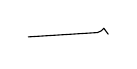
\begin{tikzpicture}[baseline=-.35ex,line cap=round,line join=round]
\draw[line width=.4pt] (0,0)--(.88,.055)
 ..controls(.92,.06)and(.94,.09)..(.96,.11)--(1.015,.035);
\end{tikzpicture}}\widehat{\pi}_1(Y,f(x)).
\]
C'est encore une condition de stabilité pour certains sous-groupes, mais pas néc. d'indice fini, de $\pi_1(X,x)$ par $\Theta$.

\margin{On peut \deleted{\unsure{généraliser}}\inserted{renforcer} cette condition, en \unsure{en supposant|ne supposant} \deleted{\unsure{tt|$\forall$}} \unsure{pas} $x'\in X'_K\cap I$, et en \deleted{\unsure{l'imposant}} exigeant que pour tt $\nu$ tel $\Theta'^\nu x'=x'$, $\Theta'^\nu$ sur $\pi_1(X',x')$, \unsure{préserve le noyau de} $f$ $\widehat{\pi}_1(Y,f(x'))$.}

4) Soient $X'_1,X'_2$ deux rev. étales finis de $X$, et $f$ un morphisme
\[
X'_1\xrightarrow{f}X'_2
\]
(\uuline{pas néc.} \uuline{un $X$-morphisme} !), $I'_1=X'_1\mathrel{\begin{tikzpicture}[baseline=-.50ex,line cap=round]
\draw[line width=.4pt] (0,-.17)--(0,.21);
\draw[line width=.4pt] (0,0)--(.10,.01);
\end{tikzpicture}} I$, $I'_2=X'_2\vert I$ on suppose \deleted{déjà que} que $J\overset{\mathrm{def}}=I'_1\cap f^{-1}(I'_2)\ne\phi$, \deleted{plus précisément que} \deleted{$\unsure{I'_1|X'_1}\cap f^{-1}(I'_2)\longrightarrow$} alors \deleted{le morph} le morphisme
\[
\Pi_1(X'_1,J)\longrightarrow\widehat{\Pi}_1(X'_2,I'_2)
\]
est compatible avec l'action 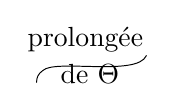
\begin{tikzpicture}[baseline=(deTheta.base),line cap=round]
\node[anchor=base west,inner sep=0pt] (deTheta) at (.27,0) {de $\Theta$};
\node[anchor=base west,inner sep=0pt] (prolongee) at (-.15,.46) {\inserted{prolongée}};
\draw[line width=.35pt] ([xshift=1pt,yshift=-1pt]prolongee.south east)
 ..controls(1.25,.08)and(.20,.31)..(.05,.16)
 ..controls(-.01,.12)and(-.03,.07)..(-.03,.01);
\end{tikzpicture} sur les groupoïdes (pour un choix compatible de cette action, s'il y a ambiguïté, cf 2°).
\mspage{100}

\scanpage{102}
A vrai dire, il ne serait pas difficile d'exiger une condition 5°) qui mette ensemble 3°) et 4°), quand on se donne non $X'_1\to X'_2$, mais
\diagram{\begin{tikzcd}[ampersand replacement=\&,row sep=3em,column sep=4em,
execute at end picture={
  \path (agA102.east) -- (agB102.west)
    coordinate[pos=.12] (agH102a) coordinate[pos=.35] (agH102b)
    coordinate[pos=.58] (agH102c) coordinate[pos=.82] (agH102d);
  \draw ([yshift=-.22em]agH102a) -- ([yshift=.32em]agH102b)
    -- ([yshift=-.22em]agH102b) -- ([yshift=.32em]agH102c)
    -- ([yshift=-.22em]agH102c) -- ([yshift=.32em]agH102d);
  \path (agB102.south) -- (agD102.north)
    coordinate[pos=.10] (agV102a) coordinate[pos=.32] (agV102b)
    coordinate[pos=.54] (agV102c) coordinate[pos=.76] (agV102d);
  \draw ([xshift=-.35em]agV102a) -- ([xshift=.35em]agV102a)
    -- ([xshift=-.35em]agV102b) -- ([xshift=.35em]agV102b)
    -- ([xshift=-.35em]agV102c) -- ([xshift=.35em]agV102c)
    -- ([xshift=-.35em]agV102d) -- ([xshift=.35em]agV102d);
}]
|[alias=agA102]| X'_1 \arrow[r,"\deleted{f_1}"] \arrow[dr,"f_1"] \&
|[alias=agB102]| \deleted{\unsure{Y_1}} \arrow[d,"\deleted{f}"] \\
X'_2 \arrow[r,"f_2"] \& |[alias=agD102]| Y_{\unsure{\deleted{2}|2}}
\end{tikzcd}}
avec $f_2$ \deleted{\unsure{ét.}} induisant un hom \deleted{\unsure{fibrant}} surjectif sur les $\pi_1$, de sorte que $\widehat{\Pi}_1(Y,f_2(I'_2))$ peut s'interpréter comme un quotient de $\widehat{\Pi}_1(X'_2,I'_2)$, de sorte que l'action \deleted{de} $\Theta'_2$ de $\Theta$ sur ce dernier passe à $\widehat{\Pi}_1(Y,f_2(I'_2))$ \ldots

Mais je ne suis pas sûr si j'aurai besoin de cette généralisation commune de 3° et 4° (et $=$ de 2°, 3°, 4°, à vrai dire !).

Les conditions 2° à 4° sont pour moi surtout une \uline{recette} commode pour trouver des conditions nécessaires sur les paramètres virtuels qui repèrent un $u\in\Gamma$ indéterminé, pour qu'ils soient effectifs i.e. proviennent bel et bien d'un $u$. Le point de vue \inserted{ici} n'est nullement de dégager \deleted{des} \unsure{condition|conditions} néc. et suff. qui permettra de \uline{caractériser} les $\Theta$ provenant de $\Gamma$ \ldots
\mspage{101}

\scanpage{103}
\hrulefill

Soit $X/K$, et soit $T$ une partie de
\inserted{\tikz[baseline=0pt,x=1em,y=1ex]{
  \node[inner sep=0pt] at (0,1.8) {$X=$};
  \draw[line width=.4pt] (-.65,1.0) .. controls (-.3,.45) and (.45,.55) .. (.45,-.1) -- (.62,-1.8);
}}$X_{\mathbb C}(\mathbb C)$, loc.\textsuperscript{t} fermée 1-connexe. Soit $X'$ \deleted{une variété algébrique}\inserted{$-X$ un} $K$-morphisme, qui sur \deleted{la partie de} un voisinage de $T$ soit fini étale. Alors $X'\vert T=X'_T$ se décompose en un nb fini de copies de $T$ -- il y a une relation d'équivalence dans $X'_T$, qu'on appelle la $T$-adjacence de points de $X'$ au dessus de $T$. On se donne \deleted{$I\subset X'_T$} $x',y'\in X'_T$
% The following small baseline trace is distinct from the overwork on the inserted T.
\unsure{\tikz[baseline=0pt,x=1ex,y=1ex]{
  \draw[line width=.45pt] (.6,.8) -- (.32,.58)
    .. controls (-.05,.55) and (-.18,.2) .. (.05,.08)
    .. controls (.38,-.02) and (.4,.3) .. (.28,.44)
    .. controls (.35,-.1) and (.15,-.5) .. (.05,-.7);
}}
\inserted{$T$ adjacents;}
\margin{\unsure{en supp.\textsuperscript{t}|en supposant} $x',y'\in X'_{\overline K}$}
si $u\in\Gamma$, on ne peut affirmer que \deleted{\unsure{ils le soient}}\inserted{$u(x'),u(y')$} soient encore $T$ adjacents.
Mais s'ils le sont, on peut regarder $l^T_{y',x'}:x'\to y'$ \inserted{``$T$-horizontal''} dans \deleted{$\unsure{\in}\,\unsure{\widehat{\Pi}_1(X'_{\overline K},x',y')}$} $\operatorname{Hom}_{\widehat{\Pi}_1(X'_{\overline K})}(x',y')$ et son transformé, \deleted{\unsure{le} \illegible{1} \unsure{de} $T$ qui passe par $x',y'$} \deleted{et son transformé} et le \uline{comparer} \deleted{$\unsure{u(l_{y',x'})}$}. : $l^T_{u(y'),u(x')}$ (qui est défini par hyp. d'horizontalité)
% The period belongs physically just after the cancelled lower formula;
% the separate colon is higher, after comparer.
\[
(53)\qquad \deleted{\unsure{u}}{}^u l^T_{y',x'}=g^T_{x,y}(u)\,l^T_{u(y'),u(x')}
\]
où
\[
g^{T\deleted{\unsure{u}}}_{x,y}(u)\in\widehat{\pi}_1\bigl(X',
\underset{\substack{\text{strate horizontale}\\\text{de }X'_T\text{ qui contient}\\u(x'),u(y')}}{
  \tikz[baseline=(term.base)]{
    \node[inner sep=0pt] (term) {$T(u x',u y')$};
    \draw[line width=.4pt]
      ([yshift=-1pt]term.south west) -- ([yshift=-4pt]term.south west)
      -- ([yshift=-4pt]term.south east) -- ([yshift=-1pt]term.south east);
  }
}\bigr)
\]
Ceci posé, on aura
\[
(54)\qquad \widehat f\underbrace{\bigl(g^T_{y',x'}(u)\bigr)}_{\substack{\rotatebox{-90}{$\in$}\\\widehat{\pi}_1(X,T)}}=g^T_{y,x}(u)
\]
\mspage{102}

\scanpage{104}
Pour \unsure{que} \deleted{strate}\inserted{comp. conn.} $T_\alpha$ de $X'_T$, considérons
\[
\widehat\varphi_\alpha:\widehat\pi_1(X'_{\overline K},T_\alpha)\longrightarrow\widehat\pi_1(X,T)
\]
(c'est un hom injectif si $X'$ rev. étale de $X$, et alors les \deleted{\unsure{différentes im.}} images des $\varphi_\alpha$ sont les conjugués de l'image de l'un d'eux). Donc \inserted{si \deleted{\unsure{on peut}} la condition sur $x'_\alpha,y'_\alpha$ est vraie pour tt $\alpha$,} la formule 54 implique ``la'' condition intrigante
\[
(55)\qquad g^T_{y,x}(u)\in\bigcap_{\alpha\in\pi_0(X'_T)}\operatorname{Im}\widehat\varphi_\alpha
\qquad\forall u\in\Gamma=\Gamma_{\overline K/K}
\]
\margin{Si $X'$ est un rev. étale de $X$, l'ens \inserted{$E=\pi_0(X'_T)$} discret \deleted{est} d'une ``fibre'' qui décrit $X'$ en termes de $\pi=\pi_1(X,T)$, via le ``foncteur-fibre'' $\mathcal E$ défini par $T\mathrel{\vcenter{\hbox{\begin{tikzpicture}[x=1em,y=1em]\draw[line width=.4pt,line cap=round] (0,0) -- (1.35,0) .. controls (1.40,0) and (1.42,-.02) .. (1.43,-.12);\end{tikzpicture}}}}X$ ($T$ 1-connexe) -- une action de $\pi$ sur $E$, et le 2\textsuperscript{e} mb de (55), est le sous-groupe \inserted{dist.} de $\pi$ noyau de $\pi\mathrel{\vcenter{\hbox{\begin{tikzpicture}[x=1em,y=1em]\draw[line width=.4pt,line cap=round] (0,0) -- (1.6,.06);\draw[line width=.65pt,line cap=round] (1.6,0) -- (1.6,.13);\end{tikzpicture}}}}\mathfrak S_E$}

C'est là une condition arithmétique, nécessaire pour que le revêt \inserted{étale} fini topologique $X'$ de $X$ (p. ex se borner à ce cas) puisse \deleted{se représenter} être muni d'une \deleted{$K$-} structure de $K$-schéma, pour laquelle $f:X'\mathrel{\vcenter{\hbox{\begin{tikzpicture}[x=1em,y=1em]\draw[line width=.4pt,line cap=round] (0,0) -- (1.35,.10) .. controls (1.40,.10) and (1.42,.08) .. (1.43,-.04);\end{tikzpicture}}}}X$ soit rat$ /K$, et telle que \deleted{$\unsure{x',y'|x,y}$}\inserted{$\forall\alpha\in\pi_0(X'_T)$,} $\forall u\in\Gamma$, $u(x'_\alpha)$ et $u(y'_\alpha)$ soient $T$-adjacents (Ce qui est une condition nettement plus faible que celle que $x',y'\in X'_K$ \deleted{)} \inserted{i.e. $x',y'$} fixes sous $\Gamma$)\ldots
\mspage{103}

\scanpage{106}
\figure{\begin{tikzpicture}[x=.0072cm,y=-.0072cm,line width=.6pt,line cap=round,line join=round,font=\scriptsize]
% Figure 1: upper left.
\node[anchor=west] at (35,42) {6 sommets};
\node[anchor=west] at (23,100) {9 flèches};
\node[anchor=west] at (352,48) {\deleted{\unsure{1}}\inserted{2} relations};
\draw[gray!45,line width=.3pt] (426,192)--(545,191);
\draw[gray!45,line width=.3pt] (248,378)--(336,402);
\draw[gray!45,line width=.3pt] (659,417)--(771,378);
\draw[gray!40,line width=.3pt] (430,185) .. controls (438,119) and (548,125) .. (546,191) .. controls (536,266) and (420,261) .. (430,185);
\draw[gray!40,line width=.3pt] (249,378) .. controls (250,311) and (340,298) .. (337,402) .. controls (328,454) and (238,441) .. (249,378);
\draw[gray!40,line width=.3pt] (660,415) .. controls (659,328) and (766,325) .. (771,379) .. controls (785,460) and (676,473) .. (660,415);
\draw[->] (430,181) .. controls (437,121) and (543,119) .. (548,180);
\draw[->] (541,208) .. controls (533,265) and (429,266) .. (432,201);
\node at (499,104) {$\lambda^\infty_+$};
\node at (490,267) {$\lambda^\infty_-$};
\node at (496,176) {$\infty$}; \fill (488,192) circle (1.4);
\draw[->] (335,401) .. controls (357,307) and (264,292) .. (252,366);
\draw[->] (247,384) .. controls (242,445) and (307,447) .. (331,414);
\node at (323,304) {$\lambda^0_+$};
\node at (277,454) {$\lambda^0_-$};
\node at (300,376) {$0$}; \draw[line width=.35pt] (287,389) circle (2.8);
\draw[->] (765,374) .. controls (746,308) and (662,320) .. (658,404);
% Literal short returning hook at the right endpoint; no second arrowhead asserted.
\draw (765,374) .. controls (763,370) and (758,370) .. (754,372);
\draw[->] (663,429) .. controls (694,477) and (769,471) .. (768,392);
\node at (708,303) {$\lambda^1_+$};
\node at (742,478) {$\lambda^1_-$};
\node at (716,375) {$1$}; \draw[line width=.55pt] (713.5,398) .. controls (713.2,393) and (718.6,392.7) .. (718.7,397.2);
\draw[->] (425,192) .. controls (91,231) and (97,341) .. (242,375);
\draw[->] (771,376) .. controls (890,287) and (695,205) .. (551,193);
\draw[->] (341,404) .. controls (427,425) and (568,427) .. (655,418);
\node at (209,217) {$a^1$};
\node at (780,235) {$a^0$};
\node at (490,386) {$a^\infty$};
\foreach \x/\y in {426/192,544/192,248/378,336/402,660/417,771/378} \fill (\x,\y) circle (3.5);
% Figure 2: upper right.
\node[anchor=west] at (801,43) {4 sommets, 1 relation};
\node[anchor=west] at (796,87) {6 flèches};
\draw[gray!45,line width=.3pt] (1310,204) .. controls (1090,192) and (939,222) .. (937,296) .. controls (929,362) and (1046,399) .. (1138,398);
\draw[gray!45,line width=.3pt] (1138,398) .. controls (1241,433) and (1376,417) .. (1468,377);
\draw[gray!45,line width=.3pt] (1088,393)--(1138,398)--(1468,377)--(1579,342);
\draw[gray!45,line width=.3pt] (1579,342) .. controls (1686,279) and (1582,214) .. (1310,204);
\draw[gray!40,line width=.3pt] (1309,205) .. controls (1313,135) and (1200,130) .. (1191,203) .. controls (1194,283) and (1305,284) .. (1309,205);
\draw[->] (1310,210) .. controls (1297,290) and (1190,273) .. (1191,202) .. controls (1186,129) and (1306,120) .. (1314,191);
\node at (1259,116) {$\Lambda^\infty_+$};
\node at (1256,213) {$\infty$};
\draw[->] (1138,405) .. controls (1124,455) and (1022,453) .. (1041,376) .. controls (1052,299) and (1135,306) .. (1141,387);
\draw[->] (1041,376) .. controls (1019,451) and (1122,455) .. (1139,408);
\node at (1015,385) {$\Lambda^0_+$};
\node at (1088,394) {$0$};
\draw[->] (1148,398) .. controls (1244,406) and (1361,402) .. (1457,382);
\node at (1302,365) {$a^\infty$};
\draw[->] (1577,338) .. controls (1535,291) and (1484,305) .. (1471,368);
\draw[->] (1470,386) .. controls (1481,437) and (1591,433) .. (1580,351);
\node at (1508,283) {$\lambda^1_+$};
\node at (1540,449) {$\lambda^1_-$};
\node at (1533,372) {$1$};
\draw[->] (1583,340) .. controls (1692,261) and (1464,205) .. (1319,204);
\node at (1525,199) {$a^0$};
\foreach \x/\y in {1310/204,1138/398,1468/377,1579/342} \fill (\x,\y) circle (3.5);
\node[text=gray!75] at (1293,531) {\unsure{3|2} cas};
% Figure 3: cancelled middle-left draft. Cancellation strokes are drawn below.
\draw[gray!50,line width=.35pt] (349,629) ellipse (72 and 64);
\draw[gray!50,line width=.35pt] (659,628) ellipse (57 and 64);
\draw[gray!50,line width=.35pt] (281,812) ellipse (47 and 58);
\draw[gray!45,line width=.35pt] (424,622) .. controls (167,632) and (105,719) .. (238,797) .. controls (374,882) and (656,855) .. (805,756) .. controls (820,695) and (746,654) .. (710,645);
\draw[gray!40,line width=.3pt] (286,628)--(424,622);
\draw[gray!40,line width=.3pt] (238,797)--(330,832);
\draw[gray!40,line width=.3pt] (602,622)--(710,645);
\node at (349,616) {$\infty$};
\node at (669,629) {$1$};
\node at (278,814) {$0$};
\node[text=gray!75] at (492,543) {\unsure{3|1} cas};
\draw[->] (598,621) .. controls (544,608) and (485,610) .. (433,622);
\draw (424,640) .. controls (410,710) and (306,711) .. (291,623);
\draw[->] (330,832) .. controls (520,871) and (800,846) .. (815,765) .. controls (820,712) and (763,667) .. (720,649);
\draw[->] (328,815) .. controls (322,730) and (261,729) .. (243,793);
\draw[->] (242,798) .. controls (222,874) and (296,891) .. (327,839);
% Pointed downward ending on the upper-right side of the cancelled 0-circle.
\draw (320,807)--(325,820)--(328,809);
\foreach \x/\y in {424/622,602/622,710/645,330/832} \fill (\x,\y) circle (2.9);
\draw[line width=.75pt] (167,775)--(449,494) (195,802)--(471,526) (239,796)--(488,552) (282,803)--(526,556);
\draw[gray!65,line width=1pt] (192,795) .. controls (450,461) and (457,515) .. (290,800) .. controls (569,467) and (591,589) .. (437,785) .. controls (716,471) and (702,633) .. (577,786) .. controls (737,571) and (700,746) .. (634,808) .. controls (701,813) and (742,791) .. (768,777);
\draw[line width=.65pt] (289,787) .. controls (471,546) and (546,455) .. (524,530) .. controls (509,580) and (422,687) .. (448,689) .. controls (618,494) and (583,603) .. (510,701) .. controls (489,752) and (537,738) .. (562,722) .. controls (685,502) and (662,606) .. (610,693) .. controls (551,782) and (657,687) .. (672,663) .. controls (721,654) and (608,785) .. (636,807);
% Figure 4: middle right.
\node[anchor=west] at (796,579) {2 sommets, \unsure{troi|trois} flèches};
\node[anchor=west] at (846,625) {0 relation};
\draw[gray!50,line width=.3pt] (1219,688) ellipse (56 and 49);
\node at (1223,684) {$\infty$};
\draw[gray!45,line width=.35pt] (974,871) .. controls (800,844) and (823,722) .. (1219,687) .. controls (1548,685) and (1611,774) .. (1463,829);
\draw[gray!40,line width=.3pt] (974,871)--(1064,872);
\draw[gray!40,line width=.3pt] (1357,855)--(1463,829);
\draw[->] (1065,861) .. controls (1055,796) and (976,792) .. (971,871) .. controls (969,932) and (1044,942) .. (1066,882);
\fill (973,871) circle (2.2); \fill (1064,872) circle (3.2);
\node at (1018,875) {$0$};
\node at (1091,775) {$\Lambda^0_+=(\Lambda^0_-)^{-1}$};
\draw[->] (1072,872) .. controls (1154,878) and (1279,878) .. (1347,859);
\node at (1219,845) {$a^\infty$};
\draw[->] (1359,866) .. controls (1367,938) and (1479,930) .. (1467,840) .. controls (1458,753) and (1372,764) .. (1358,844);
\draw (1364,886) .. controls (1371,902) and (1391,910) .. (1406,905);
\draw (1464,810) .. controls (1476,816) and (1474,824) .. (1466,834);
\fill (1357,855) circle (3.2);
\node at (1422,846) {$1$};
\node at (1513,933) {$\Lambda^{\prime1}_-=(\Lambda^{\prime1}_+)^{-1}$};
\node[text=gray!75] at (1260,1006) {\unsure{3|2} cas};
% Figure 5: lower left.
\node[anchor=west] at (39,992) {1 sommet};
\node[anchor=west] at (42,1050) {2 flèches};
\node[anchor=west] at (296,940) {0 relation};
\draw[gray!45,line width=.35pt] (534,1071) ellipse (50 and 56);
\fill[gray!75] (488,1077) circle (2.0); \fill[gray!75] (580,1076) circle (2.0);
\node at (538,1072) {$\infty$};
\draw[gray!45,line width=.35pt] (328,1253) .. controls (123,1249) and (129,1109) .. (488,1077) .. controls (759,1066) and (887,1111) .. (793,1189);
\draw[gray!40,line width=.3pt] (328,1253)--(438,1259);
\draw[gray!40,line width=.3pt] (692,1218)--(793,1189);
% Separate short upright/hooked residue on the pale chord, without vertex semantics.
\node[anchor=base west,inner sep=0,outer sep=0] at (789,1187) {\unsure{\begin{tikzpicture}[x=.0072cm,y=-.0072cm,line width=.45pt,line cap=round,line join=round,baseline=0pt]\draw (0,-5) .. controls (1.5,-3) and (1.3,1) .. (1,3) .. controls (2,6) and (5,4.5) .. (4,2);\end{tikzpicture}}};
\draw[gray!40,line width=.3pt] (433,1254) .. controls (448,1178) and (321,1173) .. (320,1254) .. controls (320,1335) and (426,1340) .. (438,1279);
\draw[->] (437,1255) .. controls (446,1173) and (323,1175) .. (322,1250) .. controls (315,1325) and (417,1353) .. (435,1282);
\draw[->] (324,1249) .. controls (325,1176) and (431,1176) .. (438,1245);
\node at (394,1169) {$\Lambda_0^+$};
\node at (376,1258) {$0$};
\draw[->,line width=1pt] (442,1258)--(688,1218);
\draw[line width=.45pt] (444,1254) .. controls (482,1248) and (509,1252) .. (540,1244);
\draw[->] (690,1228)--(444,1273);
\node at (574,1211) {$\deleted{\unsure{a^\infty}}$};
\draw (694,1218) .. controls (687,1117) and (827,1124) .. (796,1201) .. controls (772,1295) and (718,1268) .. (694,1229);
\draw[->] (795,1201) .. controls (784,1244) and (761,1271) .. (736,1258);
\node at (758,1117) {$A_+^{01}$};
\node at (749,1209) {$1$};
\fill (438,1259) circle (3.5); \fill (692,1218) circle (3.5);
\node[text=gray!75] at (490,1440) {3 cas.};
\end{tikzpicture}}
\mspage{105}

\scanpage{108}

\figure{%
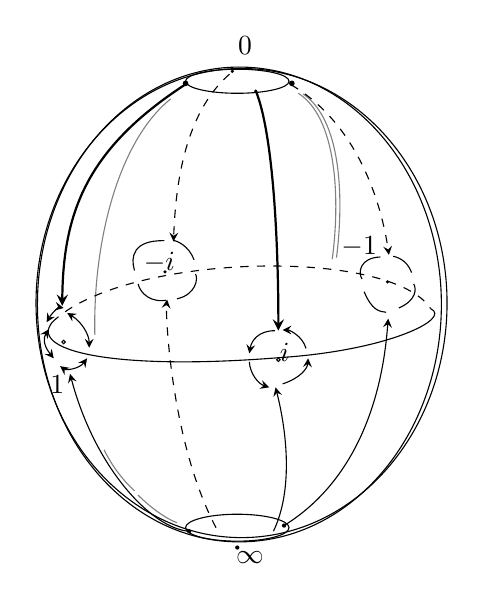
\begin{tikzpicture}[x=0.9cm,y=0.9cm,>=stealth]
\draw[thin] (0,0) ellipse (2.85 and 3.35);
\draw[thin] (0.03,0.02) ellipse (2.9 and 3.31);
% Pale left interior construction contour and separated lower fragments.
\draw[gray,thin] (-0.97,2.90) .. controls (-1.72,2.30) and (-2.07,0.85) .. (-2.04,-0.43);
\draw[gray,thin] (-1.91,-2.05) .. controls (-1.78,-2.31) and (-1.64,-2.48) .. (-1.48,-2.63);
\draw[gray,thin] (-1.43,-2.69) .. controls (-1.24,-2.88) and (-1.02,-3.03) .. (-0.88,-3.08);
% Two close pale right interior contours, ending above the back equator.
\draw[gray,thin] (0.83,2.98) .. controls (1.36,2.65) and (1.43,1.54) .. (1.31,0.64);
\draw[gray,thin] (0.90,2.97) .. controls (1.43,2.61) and (1.48,1.54) .. (1.37,0.66);

\draw (-0.03,3.15) ellipse (0.73 and 0.17);
\draw (-0.03,-3.15) ellipse (0.73 and 0.19);
\node at (0.08,3.65) {$0$};
\node at (0.15,-3.57) {$\infty$};
\draw[dashed] (-2.64,-0.25) .. controls (-1.65,0.72) and (2.13,0.82) .. (2.7,-0.06);
\draw (-2.64,-0.25) .. controls (-2.98,-0.65) and (-1.8,-0.94) .. (0.57,-0.75) .. controls (2.1,-0.65) and (3.0,-0.2) .. (2.7,-0.06);
\draw[->,thick] (-0.77,3.1) .. controls (-2.15,2.2) and (-2.49,1.3) .. (-2.5,-0.02);
\draw[<-] (-2.39,-0.98) .. controls (-2.04,-2.3) and (-1.25,-3.15) .. (-0.72,-3.2);
\draw[->,thick] (0.23,3.02) .. controls (0.5,2.35) and (0.55,0.65) .. (0.55,-0.37);
\draw[->] (0.48,-3.2) .. controls (0.76,-2.62) and (0.67,-1.8) .. (0.51,-1.17);
\draw[dashed,->] (-0.14,3.25) .. controls (-0.77,2.7) and (-0.9,1.7) .. (-0.93,0.89);
\draw[dashed,->] (-0.33,-3.15) .. controls (-0.98,-1.91) and (-1.04,-0.1) .. (-1.02,0.07);
\draw[dashed,->] (0.73,3.1) .. controls (1.75,2.5) and (2.03,1.25) .. (2.11,0.7);
\draw[->] (0.63,-3.12) .. controls (1.94,-2.31) and (2.06,-0.68) .. (2.1,-0.2);
\draw[<->] (-2.43,-0.12) .. controls (-2.22,-0.25) and (-2.12,-0.43) .. (-2.12,-0.61);
\draw[<->] (-2.15,-0.76) .. controls (-2.26,-0.91) and (-2.45,-0.93) .. (-2.53,-0.87);
\draw[<->] (-2.62,-0.76) .. controls (-2.78,-0.56) and (-2.76,-0.46) .. (-2.69,-0.35);
\draw[<->] (-2.72,-0.25) .. controls (-2.62,-0.08) and (-2.53,-0.04) .. (-2.48,-0.05);
\node at (-2.57,-1.13) {$1$};
\draw (-2.48,-0.53) circle (0.025);
\draw[->] (0.5,-0.37) .. controls (0.27,-0.37) and (0.17,-0.51) .. (0.14,-0.69);
\draw[->] (0.14,-0.81) .. controls (0.15,-0.98) and (0.27,-1.12) .. (0.42,-1.17);
\draw[->] (0.61,-1.12) .. controls (0.86,-1.04) and (0.96,-0.9) .. (0.97,-0.76);
\draw[->] (0.94,-0.62) .. controls (0.89,-0.44) and (0.7,-0.36) .. (0.61,-0.36);
\node at (0.64,-0.68) {$i$};
\draw (0.55,-0.78) circle (0.025);
\draw (-1.06,0.9) .. controls (-1.5,0.91) and (-1.54,0.67) .. (-1.48,0.48);
\draw (-1.43,0.29) .. controls (-1.36,0.05) and (-1.11,0.04) .. (-1.04,0.06);
\draw (-0.88,0.08) .. controls (-0.61,0.14) and (-0.58,0.37) .. (-0.62,0.43);
\draw (-0.64,0.63) .. controls (-0.71,0.83) and (-0.9,0.91) .. (-0.93,0.9);
\node at (-1.13,0.59) {$-i$};
\fill (-1.05,0.46) circle (0.025);
\draw (1.99,0.67) .. controls (1.7,0.66) and (1.67,0.45) .. (1.73,0.36);
\draw (1.76,0.18) .. controls (1.87,-0.08) and (1.97,-0.1) .. (2.07,-0.11);
\draw (2.25,-0.05) .. controls (2.5,0.06) and (2.5,0.22) .. (2.46,0.29);
\draw (2.43,0.45) .. controls (2.36,0.64) and (2.21,0.67) .. (2.17,0.68);
\node at (1.69,0.81) {$-1$};
\fill (2.09,0.32) circle (0.025);
\fill (-0.76,3.12) circle (0.04);\fill (0.74,3.12) circle (0.04);
\fill (-0.1,3.29) circle (0.025);\fill (0.23,3.01) circle (0.025);
\fill (-0.71,-3.2) circle (0.03);\fill (0.63,-3.12) circle (0.03);
\fill (-0.03,-3.43) circle (0.03);
\end{tikzpicture}%
}

\diagram{\begin{tikzcd}[ampersand replacement=\&,row sep=small]
z \arrow[r] \& -z \\
z \arrow[r] \& \dfrac{1}{z} \\
z \& {} \arrow[l]
\end{tikzcd}}

\diagram{\begin{tikzcd}[ampersand replacement=\&]
1 \arrow[r] \& \mathbb{F}_2^2 \arrow[r] \& \mathcal{A}_4 \arrow[r] \& \mathbb{Z}/3\mathbb{Z} \arrow[r] \& 1
\end{tikzcd}}

\figure{%
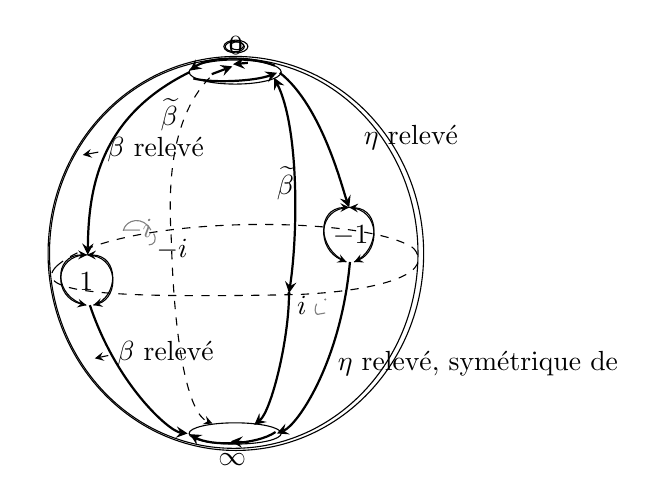
\begin{tikzpicture}[x=0.9cm,y=0.9cm,>=stealth]
\draw[thin] (0,0) ellipse (2.6 and 2.75);
\draw[thin] (0.03,0) ellipse (2.65 and 2.78);
\draw (0.02,2.56) ellipse (0.65 and 0.17);
\draw (0.02,-2.54) ellipse (0.65 and 0.15);
\node at (0.03,2.93) {$\unsure{0}$};
\draw (0.03,2.92) ellipse (0.17 and 0.09);
\draw[thin] (0.015,2.918) ellipse (0.135 and 0.072);
\draw[thin] (0.045,2.93) ellipse (0.092 and 0.055);
\node at (-0.02,-2.91) {$\infty$};
\draw[dashed] (-2.5,-0.18) .. controls (-1.7,0.55) and (1.8,0.56) .. (2.53,0.08);
\draw[dashed] (-2.5,-0.18) .. controls (-2.9,-0.58) and (-1.6,-0.63) .. (0.9,-0.58) .. controls (2.2,-0.52) and (2.84,-0.25) .. (2.53,0.08);
\draw[->,thick] (-0.62,2.56) .. controls (-1.9,1.93) and (-2.05,0.91) .. (-2.06,-0.02);
\draw[->,thick] (-2.03,-0.73) .. controls (-1.65,-1.86) and (-0.91,-2.51) .. (-0.65,-2.54);
\draw[->,thick] (0.65,2.55) .. controls (1.25,2.08) and (1.54,0.89) .. (1.63,0.65);
\draw[->,thick] (1.64,-0.12) .. controls (1.51,-1.54) and (0.9,-2.42) .. (0.61,-2.54);
\draw[dashed,->] (-0.34,2.48) .. controls (-0.93,1.87) and (-0.92,0.84) .. (-0.88,0.18) .. controls (-0.84,-1.3) and (-0.64,-2.26) .. (-0.3,-2.40);
\draw[<->,thick] (0.78,-0.56) .. controls (0.91,0.3) and (0.92,1.78) .. (0.57,2.48);
\draw[->,thick] (0.78,-0.56) .. controls (0.78,-1.22) and (0.53,-2.22) .. (0.29,-2.42);
\draw[->] (-2.07,-0.02) .. controls (-2.55,-0.02) and (-2.55,-0.62) .. (-2.08,-0.73);
\draw[->] (-2.07,-0.02) .. controls (-1.61,-0.03) and (-1.62,-0.62) .. (-1.98,-0.73);
\draw[->] (-2.08,-0.73) .. controls (-2.55,-0.62) and (-2.55,-0.02) .. (-2.07,-0.02);
\draw[->] (-1.98,-0.73) .. controls (-1.62,-0.62) and (-1.61,-0.03) .. (-2.07,-0.02);
\node at (-2.08,-0.39) {$1$};
\draw[->] (1.63,0.65) .. controls (1.17,0.64) and (1.17,0.06) .. (1.59,-0.12);
\draw[->] (1.63,0.65) .. controls (2.08,0.62) and (2.06,0.04) .. (1.7,-0.12);
\draw[->] (1.59,-0.12) .. controls (1.17,0.06) and (1.17,0.64) .. (1.63,0.65);
\draw[->] (1.7,-0.12) .. controls (2.06,0.04) and (2.08,0.62) .. (1.63,0.65);
\node at (1.65,0.25) {$-1$};
\node at (-0.87,0.05) {$-i$};
% Faint residue above-left of the live -i: its reading and deletion state remain unsure.
\node[gray] at (-1.37,0.34) {$\unsure{-i}$};
\draw[gray,thin] (-1.56,0.32) .. controls (-1.52,0.49) and (-1.27,0.53) .. (-1.17,0.33);
\draw[gray,thin] (-1.13,0.28) .. controls (-1.08,0.19) and (-1.12,0.12) .. (-1.2,0.12);
\fill (0.78,-0.56) circle (0.025);\node at (0.96,-0.73) {$i$};
% Additional pale stem/foot and detached point beside i; no deletion or chronology inferred.
\draw[gray,thin] (1.17,-0.71) .. controls (1.14,-0.77) and (1.14,-0.84) .. (1.18,-0.86) -- (1.29,-0.84);
\fill[gray] (1.29,-0.65) circle (0.016);

\node at (-0.91,1.96) {$\widetilde{\beta}$};
\node at (0.73,0.99) {$\widetilde{\beta}$};
\node[anchor=west] at (-1.92,1.46) {$\beta$ relevé};
\draw[->] (-1.91,1.43) -- (-2.13,1.39);
\node[anchor=west] at (-1.78,-1.41) {$\beta$ relevé};
\draw[->] (-1.77,-1.44) -- (-1.96,-1.48);
\node[anchor=west] at (1.7,1.64) {$\eta$ relevé};
\node[anchor=west] at (1.33,-1.55) {$\eta$ relevé, symétrique de};
\draw[->,thick] (0.58,2.65) .. controls (0.2,2.8) and (-0.36,2.77) .. (-0.62,2.58);
\draw[->,thick] (-0.57,2.47) .. controls (-0.3,2.4) and (0.3,2.43) .. (0.61,2.55);
\draw[->,thick] (-0.31,2.53) -- (-0.02,2.64);
\draw[->,thick] (0.20,2.69) -- (-0.01,2.67);
\draw[->,thick] (0.59,-2.52) .. controls (0.31,-2.71) and (-0.33,-2.72) .. (-0.62,-2.55);
\draw[->,thick] (0.21,-2.67) -- (-0.04,-2.65);
\end{tikzpicture}%
}

\[
l_{\infty}l_1l_0l_{-1}=1
\]

\mspage{107}

\scanpage{109}

\begin{center}
U N I V E R S I T E\\
DES SCIENCES ET TECHNIQUES\\
DU LANGUEDOC\\
------------
\end{center}

MONTPELLIER, le 06 Octobre 1978

Service de la Scolarité\\
MR / GJ\\
Diffusion\quad : Liste H\\
N° : 5462

\begin{center}
\uline{AVIS DE SOUTENANCE D'UNE THESE DE DOCTORAT D ' ETAT}
\end{center}

\uline{Nom et prénom du candidat} : SOONCKINDT Louis

\uline{Titre de la thèse} : Contribution à l'étude des propriétés électroniques des surfaces réelles et clivées sous ultra-vide d'antimoniure de gallium.

\uline{Date, heure et lieu de soutenance prévus} : 26 OCTOBRE 1978 à 11 Heures\\
Salle de cours n° 7 - U.S.T.L.

\uline{Nom du Directeur de thèse} : Monsieur le Professeur LASSABATERE Louis.

\uline{Désignation du Laboratoire où la thèse est préparée} : C. E. E. S.

\uline{Résumé de la thèse} : Après avoir décrit le montage expérimental réalisé au Laboratoire et permettant l'étude des travaux de sortie par la méthode de Kelvin on étudie les propriétés électroniques des surfaces réelles et des surfaces propres, obtenues par clivage, de GaSb. On précise les interactions entre les états électroniques de surface (\handwritten{\textit{intrinsèques et extrinsèques}}) dans l'obscurité et sous éclairement dans la gamme de température comprise entre 100 et $420^\circ$ K.

\uline{Durée approximative des recherches ayant abouti à la thèse} : 8 ans.

\uline{Noms des Rapporteurs} :

\diagram{$\begin{array}{lll}
\text{LASSABATERE} & \text{Louis} & \text{, Professeur, Electronique, U. S. T. L.} \\
\text{LANNOO} & \text{Maurice} & \text{Maître Recherche, Physique du Solide, ISEN LILLE} \\
\text{SEBENNE} & \text{Claude} & \text{Maître Recherche, Physique du Solide, PARIS 6}
\end{array}$}

\uline{Composition du jury proposé} :

\diagram{$\begin{array}{lll}
\text{PISTOULET} & \text{B.} & \text{Professeur, Electronique, U.S.T.L.} \\
 & & \text{Président} \\
\text{LACOSTE} & \text{R.} & \text{Professeur, Electronique, Univers. P. SABATIER, TOULOUSE} \\
\text{LANNOO} & \text{M.} & \text{Maître Recherche, Physique du Solide, ISEN LILLE} \\
\text{SEBENNE} & \text{C.} & \text{Maître Recherche, Physique du Solide, PARIS 6} \\
 & & \text{(Membre extérieur choisi en raison de sa compétence scientifique)} \\
\text{LASSABATERE} & \text{L.} & \text{Professeur, Electronique, U.S.T.L.} \\
\text{NOUGIER} & \text{J.-P.} & \text{Professeur, Electronique, U.S.T.L.} \\
 & & \text{(Membre étranger à la spécialité du candidat).}
\end{array}$}

Le Secrétaire Général,

\figure{\begin{tikzpicture}[x=.015cm,y=-.015cm]
% Signature initials tentatively read E. S.; the cursive forms are drawn in place.
\node[anchor=base west,inner sep=0pt,font=\ttfamily\normalsize] at (222,139)
  {E.\qquad S\ I\ A\ U};
\draw[line width=.35pt] (222,145) -- (427,145);
\draw[line width=.35pt] (445,27)
  .. controls (381,37) and (146,107) .. (50,143)
  .. controls (26,151) and (27,158) .. (62,153)
  .. controls (164,137) and (417,81) .. (498,60)
  .. controls (523,52) and (521,44) .. (484,46)
  .. controls (445,46) and (390,51) .. (365,58);
\node[anchor=north west,inner sep=0pt] at (286,18) {\unsure{\begin{tikzpicture}[x=.015cm,y=-.015cm,line width=.35pt]
\draw (40,12) .. controls (35,29) and (25,31) .. (17,26);
\draw (31,13) .. controls (24,24) and (8,54) .. (2,66)
  .. controls (-2,77) and (10,72) .. (17,67);
\draw (16,39) .. controls (15,50) and (28,51) .. (23,40);
\fill (31,48) circle[radius=.16mm];
\draw (50,31) .. controls (54,14) and (65,-3) .. (76,1)
  .. controls (92,7) and (78,25) .. (66,25)
  .. controls (53,24) and (57,35) .. (61,46)
  .. controls (69,61) and (57,73) .. (52,64)
  .. controls (48,58) and (53,51) .. (54,48);
\fill (79,43) circle[radius=.16mm];
\end{tikzpicture}}};
\end{tikzpicture}}

MR LE PROFESSEUR GROTHENDIECK A.

\hfill 5

MATHEMATIQUES

\mspage{108}

\scanpage{110}

\diagram{\begin{tikzcd}[ampersand replacement=\&,column sep=large,row sep=large]
\cdot E_0 \arrow[r,dash] \arrow[d, no head, to path={(\tikztostart) -- coordinate[pos=0.78] (leftbranch110) (\tikztotarget) (leftbranch110) -- ++(0.12,-0.11) \tikztonodes}] \& \pi_0(E_0)=\deleted{E_0/\pi\,\operatorname{Ssgr}}( \arrow[d] \\
\operatorname{Ssgr}(\pi) \arrow[r] \& \operatorname{Ssgr}(\unsure{\Pi|E})/\pi
\end{tikzcd}}
\diagram{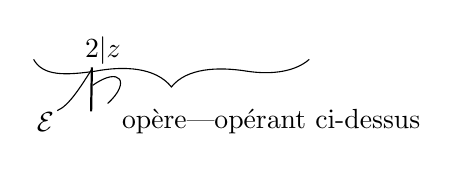
\begin{tikzpicture}[x=1cm,y=1cm]
\draw (0,0.12) .. controls (0.12,-0.10) and (0.42,-0.08) .. (0.78,-0.03)
 .. controls (1.15,0.04) and (1.55,0.02) .. (1.75,-0.23)
 .. controls (1.94,0.01) and (2.34,0.03) .. (2.71,-0.03)
 .. controls (3.04,-0.08) and (3.33,-0.03) .. (3.5,0.12);
\node at (0.88,0.23) {$\unsure{2|z}$};
\node at (0.15,-0.67) {$\mathcal{E}$};
\draw (0.30,-0.53) .. controls (0.45,-0.47) and (0.60,-0.22) .. (0.73,-0.02);
\draw[thick] (0.73,-0.54) -- (0.74,0.02);
\draw (0.75,-0.21) .. controls (1.10,0.04) and (1.24,-0.17) .. (0.94,-0.44);
\node[anchor=west] at (1.0,-0.67) {\unsure{opère|opérant} ci-dessus};
\end{tikzpicture}}

\margin{$\mathcal{E}/\pi=\Gamma$}

\diagram{\begin{tikzcd}[ampersand replacement=\&,column sep=large,row sep=small]
\mathcal{E}(=\Gamma.\pi) \& \& \mathcal{E} \arrow[dd] \\
\bigcup \& \& {} \\
\pi \arrow[r,dash] \& E_0 \arrow[r] \& \operatorname{Ssgr}(\pi)/\pi
\end{tikzcd}}

\figure{%
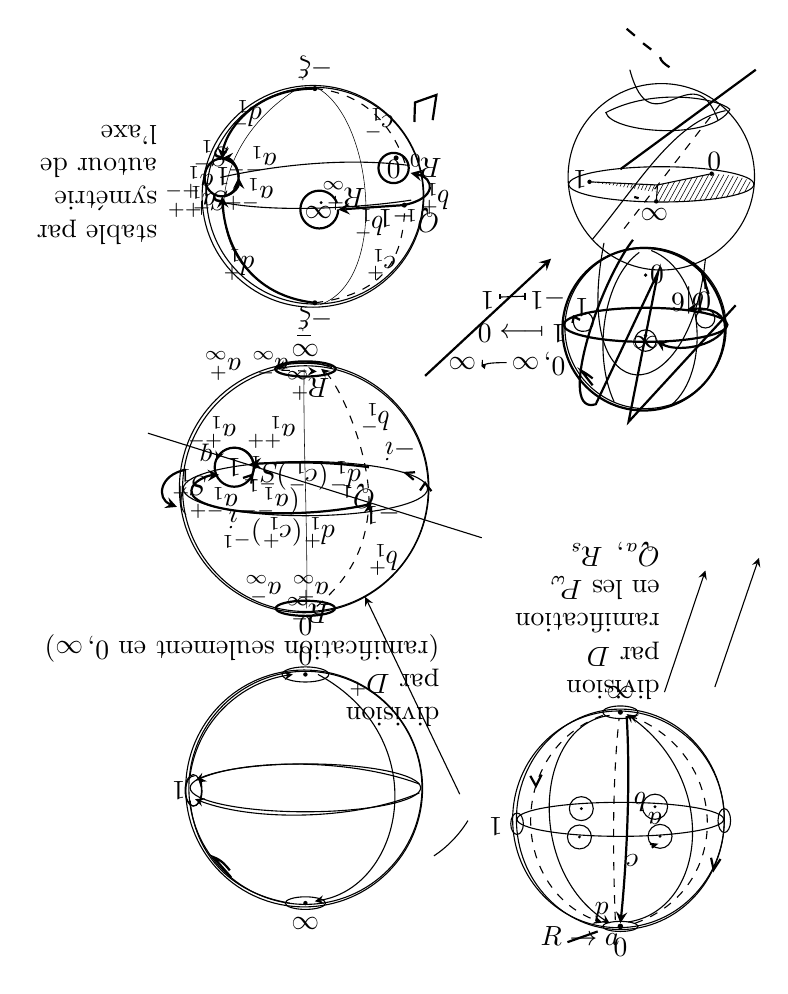
\begin{tikzpicture}[x=0.8cm,y=0.8cm,>=stealth]
\begin{scope}[rotate=180,transform shape]
\begin{scope}[shift={(0,0)}]
\draw (0,0) ellipse (1.65 and 1.75);
\draw[thin] (0.03,0) ellipse (1.68 and 1.72);
\draw[thick] (-1.59,0.63) -- (-1.48,0.80) -- (-1.44,0.61);
\draw[thick] (1.25,-0.71) -- (1.34,-0.53) -- (1.43,-0.69);
\draw (0,1.7) ellipse (0.28 and 0.08);\draw (0,-1.7) ellipse (0.28 and 0.1);
\fill (0,1.7) circle (0.045);\fill (0,-1.7) circle (0.04);
\node at (0,2.03) {$0$};\node at (0,-2.02) {$\infty$};
\draw (0,0) ellipse (1.64 and 0.27);
\draw[->,thick] (-0.1,-1.64) .. controls (-0.18,-0.3) and (-0.05,1.2) .. (0,1.65);
\draw[dashed] (0.08,1.6) .. controls (0.12,0.6) and (0.13,-0.6) .. (0.02,-1.6);
\draw[->] (-0.12,1.63) .. controls (-1.35,1.45) and (-1.6,-0.6) .. (-0.1,-1.67);
\draw[->] (0.17,-1.65) .. controls (1.37,-1.5) and (1.5,0.8) .. (0.17,1.65);
\draw[dashed,->] (-0.23,1.65) .. controls (-1.8,1.1) and (-1.73,-1) .. (-0.14,-1.65);
\draw[dashed,->] (0.28,-1.65) .. controls (1.8,-1.1) and (1.78,1.1) .. (0.29,1.64);
\draw (-0.63,0.27) circle (0.19);\fill (-0.63,0.27) circle (0.025);
\draw[thick] (-0.47,0.39) -- (-0.56,0.40) -- (-0.50,0.45);
\draw (0.65,0.28) circle (0.19);\fill (0.65,0.28) circle (0.025);
\draw (-0.55,-0.2) circle (0.2);\fill (-0.55,-0.2) circle (0.025);
\draw (0.62,-0.17) circle (0.19);\fill (0.62,-0.17) circle (0.025);
\draw (-1.65,0.02) ellipse (0.1 and 0.19);\draw (1.64,0.07) ellipse (0.1 and 0.17);
\node at (1.98,0.11) {$1$};
\node at (0.29,1.47) {$d$};\node at (-0.2,0.65) {$c$};\node at (-0.32,-0.28) {$b$};
\node at (-0.55,-0.01) {$a$};
\node[rotate=180] at (0.64,1.86) {$\deleted{\unsure{R\to a}}$};
\draw[thick] (0.36,1.78) -- (0.84,1.95);
\end{scope}
\draw (2.42,0.02) .. controls (2.56,0.25) and (2.76,0.45) .. (2.96,0.58);
\draw[->] (-1.5,-2.1) -- (-2.2,-4.15);
\draw[->] (-0.7,-2.02) -- (-1.35,-3.95);
\node[anchor=west,align=left] at (-0.78,-3.15) {division\\par $D$\\ramification\\en les $P_{\omega}$\\$Q_a,\ R_s$};

\begin{scope}[shift={(5,-0.5)}]
\draw (0,0) circle (1.85);\draw[thin] (0.02,0.01) circle (1.88);
\draw (0,0) ellipse (1.83 and 0.38);
\draw (0,1.83) ellipse (0.32 and 0.1);\draw (0,-1.8) ellipse (0.37 and 0.12);
\fill (0,1.83) circle (0.035);\fill (0,-1.8) circle (0.035);
\node at (0,2.15) {$\infty$};\node at (0,-2.08) {$0$};
\draw[->] (-0.2,-1.8) .. controls (-2.05,-0.8) and (-1.58,1.56) .. (-0.15,1.8);
\draw[->] (-1.81,0.08) .. controls (-0.8,0.51) and (0.8,0.54) .. (1.75,0.18);
\draw[->] (-1.81,-0.06) .. controls (-0.75,-0.46) and (0.9,-0.47) .. (1.74,-0.12);
\draw (1.78,0.04) ellipse (0.13 and 0.25);\draw[->] (1.76,-0.19) arc (-95:240:0.13 and 0.24);
\node at (2.01,0.04) {$1$};
\draw (1.83,0.2) .. controls (1.76,1.0) and (1.25,1.66) .. (0.25,1.83);
\draw[thick] (1.18,1.42) -- (1.46,1.10) .. controls (1.32,1.15) and (1.25,1.25) .. (1.20,1.31);
\draw[->] (1.83,-0.2) .. controls (1.7,-1.1) and (0.99,-1.68) .. (0.2,-1.8);
\end{scope}
\draw[->] (2.55,-0.4) -- (4.05,-3.53);
\node[anchor=west,align=left] at (2.72,-2.2) {division\\par $D^+$\\(ramification seulement en $\unsure{0},\infty$)};

\begin{scope}[shift={(5,-5.25)}]
\draw[thin] (0,0) circle (1.95);
\draw[thin] (0.02,-0.01) circle (1.98);
\draw (0,0) ellipse (1.94 and 0.43);
\draw[thick] (-2.00,0.04) -- (-1.90,-0.09) -- (-1.82,0.03);
\draw[thick] (-1.72,-0.14) -- (-1.59,-0.25) -- (-1.74,-0.26);
\draw[thick] (0,1.9) ellipse (0.47 and 0.12);\draw[thick] (0,-1.9) ellipse (0.48 and 0.12);
\node at (0,2.18) {$0$};\node at (0,-2.2) {$\infty$};
\draw[->,dashed] (-0.18,1.87) .. controls (-0.85,1.3) and (-0.96,0.75) .. (-1.01,0.25);
\draw[->,dashed] (-1.01,0.25) .. controls (-1.02,-0.65) and (-0.5,-1.7) .. (-0.25,-1.9);
\fill (-1.01,0.25) circle (0.04);
\draw[->,thick] (-1.01,0.25) .. controls (0.15,0.51) and (1.83,0.4) .. (1.81,0.03) .. controls (1.8,-0.12) and (1.55,-0.21) .. (1.37,-0.22);
\draw[->,thick] (-1.01,-0.34) .. controls (-0.27,-0.44) and (0.28,-0.42) .. (0.88,-0.39);
\draw[thick] (1.13,-0.34) circle (0.31);
\draw[->] (0.85,-0.19) arc (150:340:0.31);
\draw[thick] (0.86,-0.08) -- (0.84,-0.22) -- (0.99,-0.17);
\node at (1.13,-0.34) {$1$};
\node at (-1.22,0.4) {$-1$};\node at (-0.83,0.12) {$Q_1$};
\node at (-1.23,1.13) {$b_1^+$};\node at (-1.1,-1.1) {$b_1^-$};
\node at (0.43,0.71) {$d_1^+(c_1^+)^{-1}$};
\node at (0.02,-0.18) {$d_1^-(c_1^-)^{-1}$};
\node at (1.06,0.23) {$(a_1^{--}a_1^{-+})$};
\node at (1.02,-0.89) {$a_1^{++}\ a_1^{+-}$};
\node at (1.84,-0.06) {$S_1^+$};\node at (0.72,-0.27) {$S_1^-$};
\node at (1.15,0.5) {$i$};\node at (-1.5,-0.6) {$-i$};
\draw[very thin] (-0.02,1.9) .. controls (-0.04,0.6) and (0.04,-0.7) .. (0.02,-1.9);
\draw[thin] (-2.8,0.78) -- (2.5,-0.88);
\node at (1.57,-0.57) {$\unsure{q}$};
\node at (0.3,1.61) {$a_\infty^+\ a_\infty^-$};
\node at (-0.03,1.96) {$\unsure{R_\infty^-}$};
\node at (-0.03,-1.63) {$R_\infty^+$};
\node at (0.94,-1.95) {$a_\infty^-\ a_\infty^+$};
\draw[->] (-0.42,-1.92) .. controls (-0.1,-2.04) and (0.2,-2.03) .. (0.44,-1.91);
\draw[->,dashed] (0.38,-1.88) -- (-0.18,-1.86);
\draw[->,thick] (1.9,-0.3) .. controls (2.32,-0.22) and (2.37,0.16) .. (2.04,0.29);
\end{scope}

\begin{scope}[shift={(4.85,-9.9)}]
\draw[thin] (0,0) circle (1.72);\draw[thin] (0.03,0.01) circle (1.76);
\draw[very thin] (-0.08,1.73) .. controls (-1.2,1.35) and (-0.92,-1.3) .. (0,-1.73);
\draw[very thin] (0.18,1.68) .. controls (1.86,1.29) and (1.85,-0.72) .. (0.26,-1.71);
\draw[thin] (-1.53,0.07) .. controls (-0.75,0.19) and (0.63,0.28) .. (1.5,0.1);
\draw[thin] (-1.5,-0.48) .. controls (-0.57,-0.6) and (0.5,-0.51) .. (1.5,-0.29);
\draw[dashed] (0,1.7) .. controls (-1.23,1.55) and (-1.4,0.87) .. (-1.43,0.16);
\draw[dashed] (-1.43,-0.52) .. controls (-1.14,-1.37) and (-0.53,-1.66) .. (0,-1.7);
\draw[->,thick] (0,1.7) .. controls (1.16,1.57) and (1.44,0.63) .. (1.47,0.01);
\draw[->,thick] (0,-1.7) .. controls (1.02,-1.7) and (1.44,-0.96) .. (1.47,-0.58);
\fill (0,1.7) circle (0.04);\fill (0,-1.7) circle (0.04);
\node at (0,2.01) {$-\overline{\xi}$};
\node at (0,-2.02) {$-\xi$};
\node at (-1.05,1.1) {$c_1^+$};\node at (-1.01,-1.14) {$c_1^-$};
\node at (1.21,1.1) {$d_1^+$};\node at (1.09,-1.27) {$d_1^-$};
\draw[thick] (1.48,-0.29) ellipse (0.27 and 0.3);
\draw[->,thick] (1.48,0.01) arc (90:180:0.27 and 0.3);
\draw[->,thick] (1.21,-0.29) arc (180:270:0.27 and 0.3);
\node at (1.46,-0.3) {$1$};
\node at (1.66,0.06) {$S_1^+$};\node at (1.65,-0.63) {$S_1^-$};
\node at (1.96,0.1) {$a_1^{++}$};\node at (2,-0.21) {$a_1^{+-}$};
\node at (1.05,-0.02) {$a_1^{-+}$};\node at (1,-0.54) {$a_1^{--}$};
\fill (-1.42,0.15) circle (0.04);\node at (-1.29,0.35) {$-1$};\node at (-1.7,0.39) {$Q_1$};
\draw[->,thick] (-1.4,0.15) -- (-0.37,0.22);
\draw[thick] (-0.37,0.22) arc (180:-160:0.3);\node at (-0.06,0.27) {$\infty$};\fill (-0.1,0.11) circle (0.025);
\node at (-0.45,0.01) {$R_\infty^+$};\node at (-0.85,0.46) {$b_1^-$};
\draw[->,thick] (-1.4,0.15) .. controls (-1.95,0.05) and (-1.9,-0.28) .. (-1.52,-0.36);
\draw[thick] (-1.25,-0.44) circle (0.24);\node at (-1.25,-0.41) {$0$};
\fill (-1.29,-0.6) circle (0.04);\node at (-1.75,-0.47) {$R_0$};
\node at (-1.9,0.05) {$b_1^+$};
\draw[thick] (-1.87,-1.2) -- (-1.93,-1.6) -- (-1.59,-1.48) -- (-1.58,-1.17);
\node[anchor=west,align=left] at (2.35,-0.17) {stable par\\symétrie\\autour de\\l'axe};
\end{scope}

\begin{scope}[shift={(-0.4,-7.8)}]
\draw (0,0) circle (1.28);\draw[thick] (0.03,0.02) circle (1.29);
\draw[thick] (0.84,0.91) -- (1.02,0.68) .. controls (0.92,0.73) and (0.87,0.78) .. (0.84,0.80);
\draw[thick] (-1.00,-0.54) -- (-0.89,-0.89) -- (-0.75,-1.04);
\draw[thick] (-0.89,-0.89) .. controls (-0.94,-0.81) and (-0.96,-0.70) .. (-0.95,-0.62);
\draw[thick] (0,-0.05) ellipse (1.3 and 0.27);
\draw (-0.95,-0.15) circle (0.15);\draw (0.94,-0.25) .. controls (0.79,-0.20) and (0.80,0.03) .. (0.95,0.05) .. controls (1.15,0.08) and (1.16,-0.10) .. (1.14,-0.18);
\draw[thick] (1.04,-0.13) -- (1.14,-0.18) -- (1.16,-0.08);\draw (0,0.2) circle (0.17);
\fill (0,0.12) circle (0.03);
\draw[->,thick] (-1.28,-0.02) .. controls (-1.1,0.32) and (-0.47,0.38) .. (-0.17,0.2);
\draw[->,thick] (-1.27,-0.03) .. controls (-1.23,-0.3) and (-0.9,-0.32) .. (-0.65,-0.29);
\node at (-0.93,-0.42) {$\deleted{\unsure{0}}$};
\node at (-0.67,-0.43) {$\deleted{\unsure{b|6}}$};\node at (1.01,-0.33) {$\deleted{1}$};\node at (0,0.23) {$\deleted{\infty}$};
\fill (0,-0.84) circle (0.03);\node at (-0.18,-0.85) {$\deleted{0}$};
\draw (-0.4,1.23) .. controls (-1.05,0.7) and (-0.94,-0.9) .. (-0.09,-1.23);
\draw (0.5,1.17) .. controls (0.85,0.4) and (0.66,-0.8) .. (0.1,-1.2);
\draw[thick] (-1.43,-0.36) -- (0.27,1.49) -- (-0.2,-0.89) -- (0.79,1.21) .. controls (1.4,1.4) and (0.8,-0.6) .. (0.2,-1.4);
\draw (-0.95,-1.1) .. controls (-0.7,1.4) and (1.2,1.4) .. (0.66,-1.35);
\end{scope}
\begin{scope}[shift={(-0.65,-10.2)}]
\draw (0,0) circle (1.48);\draw (0,0.12) ellipse (1.47 and 0.28);
\fill (-0.8,-0.05) circle (0.035);\node at (-0.84,-0.24) {$\deleted{0}$};
\fill (0.08,0.39) circle (0.035);\node at (0.11,0.59) {$\deleted{\infty}$};
\draw[thick] (0.36,0.34) -- (0.43,0.32);
\fill (1.14,0.08) circle (0.035);\node at (1.29,0.04) {$\deleted{1}$};
\draw[thin] (-0.8,-0.05) -- (0.06,0.13) -- (0.08,0.39);
\draw[thin] (0.06,0.13) -- (1.14,0.08);
\begin{scope}
\clip (-1.46,0.12) .. controls (-1.3,0.38) and (-0.45,0.42) .. (0.08,0.39) -- (0.06,0.13) -- (-0.8,-0.05) .. controls (-1.13,-0.03) and (-1.42,0.02) .. (-1.46,0.12);
\foreach \xx in {-1.6,-1.52,...,0.16} {\draw[very thin] (\xx,-0.12) -- ++(0.34,0.62);}
\end{scope}
\begin{scope}
\clip (0.06,0.13) -- (1.14,0.08) -- (0.1,0.24) -- cycle;
\foreach \xx in {0,0.06,...,1.2} {\draw[very thin] (\xx,0.03) -- ++(0.12,0.27);}
\end{scope}
\draw (-1.02,-1.05) .. controls (-0.2,-0.88) and (0.35,0.1) .. (1.1,1.0);
\draw[dashed] (-0.94,-1.16) -- (0.65,0.9);
\draw[thick] (-1.5,-1.7) -- (0.65,-0.12);
\draw (-1.09,-1.07) .. controls (-0.8,-0.56) and (0.8,-0.7) .. (0.88,-1.02) .. controls (0.1,-1.43) and (-0.92,-1.24) .. (-1.09,-1.07);
\draw (-0.9,-0.9) .. controls (-0.5,-2) and (0.15,-0.4) .. (0.5,-1.7);
\draw[thick] (-0.13,-1.74) .. controls (-0.05,-1.79) and (0.01,-1.84) .. (0.02,-1.90);
\draw[thick] (0.16,-2.02) -- (0.29,-2.12);
\draw[thick] (0.42,-2.24) -- (0.55,-2.35);
\end{scope}
\draw[->,thick] (3.1,-7.04) -- (1.1,-8.9);
\node[align=left] at (1.8,-7.73) {$0,\infty\,\tikz[baseline=-0.4ex,x=1em,y=1em]{\draw (0,0) .. controls (0.34,0) and (0.65,0.01) .. (0.80,0.07) -- (0.88,0.08) -- (0.87,-0.10);\draw[thick] (0.79,0.07) -- (0.81,0.16) -- (0.89,0.09);}\,\infty$\\$1\longmapsto0$\\$-1\,\tikz[baseline=-0.4ex,x=1em,y=1em]{\draw (0,0) -- (0.90,0.03);\draw (0,-0.13) -- (0,0.13);\draw[thick] (0.90,0.10) -- (0.90,-0.08);}\,1$};
\end{scope}
\end{tikzpicture}%
}

\mspage{109}

\scanpage{111}

\[
\Sigma_J=\mathbb{P}(V(J))\simeq\check{\mathbb{P}}(V(J))
\]
\diagram{\begin{tikzcd}[ampersand replacement=\&]
\cdot \arrow[r,dash] \& V(J) \arrow[r] \& \mathcal{O}^J \arrow[r,"\text{somme}"',/tikz/arrows={-|}] \& \mathcal{O} \arrow[r] \& 0
\end{tikzcd}}

\deleted{Suite}
\diagram{\begin{tikzcd}[ampersand replacement=\&]
0 \arrow[r] \& F \arrow[r] \& V(J)_\Sigma \arrow[r] \& \mathcal{O}_\Sigma(1) \arrow[r,dash] \& 0
\end{tikzcd}}

\[
F(1)\simeq\mathcal{O}(\omega)
\qquad
(\mathcal{O}\ \text{tordu par }\underline{\omega}=\underline{\omega}(J)\deleted{\unsure{)}},\ \text{i.e. }\det V(J))
\]
\[
\mathcal{O}(1)\simeq\check{F}(\omega)
\qquad
\left(\text{par }F\wedge\underline{\mathcal{O}}_\Sigma(1)
\mathrel{\mathop{\simeq\!\longrightarrow}\limits_{\text{prod. ext.}}}
\det V(J)_\Sigma\simeq\mathcal{O}_\Sigma(\omega){}_{\deleted{\Sigma}}\right)
\]
\margin{attention signes!}
\margin{$+$}

\margin{%
$F\times V(J)\longrightarrow\underline{\mathcal{O}}$

Accouplement donné (\deleted{fixant} un ordre circulaire fixé \deleted{en prenant} $(i,j,k)$), par
$x\wedge y\wedge e_i=x\wedge y\wedge e_j=x\wedge y\wedge e_k$
où $x\in F$, $y\in V(J)$ mod $F$
i.e. donné par les \inserted{\unsure{3|2}} mineurs -
de la matrice de $(x,y)$.
}

\[
\underline{\Omega}^1_\Sigma\deleted{\unsure{0}}\simeq F(-1)\simeq\mathcal{O}(\unsure{-2})(\underline{\omega})
\]
\[
\underline{\check{\Omega}}^1_\Sigma\simeq\mathcal{O}(2)(\underline{\omega})
\qquad\text{fibré tangent : }\Sigma
\]

\margin{$\deleted{\unsure{\varphi_{ij}+\varphi_{jk}+\varphi_{ki}=0}}$}

Points 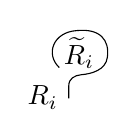
\begin{tikzpicture}[baseline=(base.base),x=1cm,y=1cm]
\node[inner sep=0pt] (base) at (-0.46,-0.57) {$R_i$};
\node[inner sep=0pt] (r) at (0,0) {$\inserted{\widetilde{R}_i}$};
\draw (-0.25,-0.19)
 .. controls (-0.43,-0.02) and (-0.33,0.26) .. (-0.03,0.28)
 .. controls (0.27,0.31) and (0.39,0.16) .. (0.36,-0.06)
 .. controls (0.34,-0.22) and (0.16,-0.27) .. (0.03,-0.28)
 .. controls (-0.06,-0.29) and (-0.13,-0.33) .. (-0.13,-0.42)
 -- (-0.13,-0.58);
\end{tikzpicture} $(i\in J)$ (``trous'') de $\Sigma$ et $P\Sigma$

\[
\begin{gathered}
R_i\subset\unsure{\mathbb{V}|V}(J)\\
\Vert\\
\mathcal{O}_{\unsure{k|\Sigma}}(e_k-e_j)\\
\simeq\mathcal{O}(\underline{\omega})
\end{gathered}
\qquad\mathcal{O}(1)_{R_i}\simeq\mathcal{O}
\]
en associant à $e_k-e_j$ l'orientation $(i,j,k)$

\margin{%
$\widetilde{R}_i$ pt au-dessus de $R_i$
image de $e_i-e_j=\varphi_{ji}$
$(\equiv e_i-e_k)$ dans $V(J)/R_i$
}

\deleted{Points les $\widetilde{R}_i$ de $P\Sigma_J=\check{V}^{*}(\mathcal{O}_\Sigma(1))$ l'élément $1$ au-dessus de $R_i$.}

\[
\Gamma(\Sigma_{\deleted{J}},\mathcal{O}_\Sigma(1))\simeq V(J)
\]
\deleted{$e_j-e_k$ section $\omega_{j,k}$}
\[
\varphi_{jk}=e_k-e_j\in\Gamma(\Sigma,\underline{\mathcal{O}}_\Sigma(1))
\]
nulle en $R_i$
\[
\varphi_{kj}=-\varphi_{jk}\qquad\varphi_{jk}(R_i)=0
\]
\margin{$\varphi_{ij}+\varphi_{jk}+\varphi_{ki}=0$.}
\[
\boxed{\varphi_{jk}(R_k)=\widetilde{R}_k\quad\varphi_{jk}(R_j)=-\widetilde{R}_j}
\]
\margin{attention signes!}

Points $Q_i$ $(i\in J)$, $Q_i^\omega{}_{\deleted{\unsure{\omega}}}$ $(i\in J,\omega\in\underline{\omega})$

\[
\begin{gathered}
Q_i\subset\unsure{\mathbb{V}|V}(\underline{J})\\
\Vert\\
\mathcal{O}(-2e_i+\deleted{\unsure{0}}(e_j+e_k))
\end{gathered}
\qquad\mathcal{O}(1)_{Q_i}\simeq\mathcal{O}(\underline{\omega})
\]

\margin{%
les deux points privilégiés de $\mathcal{O}(\omega)_{Q_i}^{*}$,
indexés par $\underline{\omega}$ sont notés $Q_i$, $Q'_i$,
ou $Q_{i,\omega}$ $((i,\omega)\in J\times\underline{\omega}$
}

\inserted{\figure{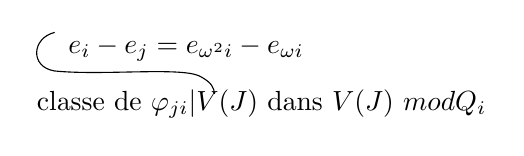
\begin{tikzpicture}[x=1cm,y=1cm]
\node[anchor=west] (eq) at (0,0.7) {$e_i-e_j=\unsure{e_{\omega^2i}-e_{\omega i}}$};
\node[anchor=west] (cl) at (-0.4,0) {classe de $\deleted{\unsure{\varphi_{ji}|V(J)}}$ dans $V(J)\ \text{mod }Q_i$};
\draw (-0.05,0.91) .. controls (-0.34,0.84) and (-0.37,0.47) .. (-0.05,0.42)
 .. controls (0.55,0.36) and (1.52,0.47) .. (1.78,0.36)
 .. controls (1.96,0.27) and (1.97,0.2) .. (1.98,0.13);
\end{tikzpicture}}}

\deleted{par $\varphi_{\omega i,\omega^2i}(Q_i)=$}

\[
\boxed{Q_i^\omega{}_{\deleted{\unsure{\omega}}}=
\underset{\deleted{\unsure{\varphi_{i,\omega^2i}}}}
{\overset{\inserted{\varphi_{\omega i,i}}}
{\deleted{\unsure{\varphi_{i,\omega i}}}}}(Q_i)}
\]

\margin{NB $\boxed{Q_i^{\omega^{-1}}{}_{\deleted{\unsure{\omega^{-1}}}}=-Q_i^\omega{}_{\deleted{\unsure{\omega}}}}$

$\varphi_{\omega i,\omega^2i}(Q_i)=2Q_i^\omega{}_{\deleted{\unsure{\omega}}}$}

donc
\[
\widetilde{Q}_i=\varphi_{jk}(Q_i),\quad
\widetilde{Q}'_i=-\varphi_{jk}(Q_i)=\varphi_{kj}(Q_i)
\]

Points $P_\omega$ $(\omega\in\underline{\omega}_J)$,
$P_i^\omega{}_{\deleted{\unsure{\omega}}}$ $(i\in J,\omega\in\omega)$.
Soit $\zeta$ une \deleted{$\unsure{\zeta}$} racine primitive cubique de $1$ (on prendra \deleted{$\unsure{\zeta}$}
\[
\zeta=\exp 2i\pi/3
\]
alors

\mspage{110}

\scanpage{112}

Carte régulière (orientée)\\
du polygône régulier $P_n$ $(n\geq2)$

en le trouant en les sommets et les centres des faces \uline{et} les milieux des segments

% The three small leaders belong to the three asterisks.  The small dark dot
% above the right asterisk is copied as ink, without assigning it a new meaning.
\figure{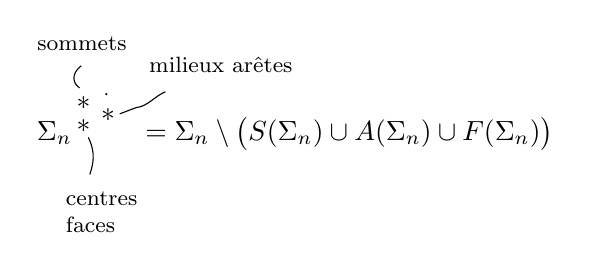
\begin{tikzpicture}[baseline=(base.base)]
\node[anchor=base] (base) at (0,0) {$\Sigma_n$};
\node at (.37,.48) {$*$};
\node at (.37,.18) {$*$};
\node at (.68,.32) {$*$};
\node at (.66,.58) {$\scriptstyle\unsure{\cdot}$};
\node[anchor=base west] at (1.03,0)
 {$=\Sigma_n\setminus\bigl(S(\Sigma_n)\cup A(\Sigma_n)\cup F(\Sigma_n)\bigr)$};
\node[font=\footnotesize,anchor=south] at (.35,1.02) {sommets};
\draw (.34,.95) .. controls (.20,.84) and (.24,.72) .. (.32,.67);
\node[font=\footnotesize,align=left,anchor=north] at (.60,-.53) {centres\\faces};
\draw (.43,.04) .. controls (.53,-.16) and (.49,-.30) .. (.45,-.43);
\node[font=\footnotesize,anchor=south west] at (1.08,.74) {milieux arêtes};
\draw (.83,.34) -- (1.04,.42) .. controls (1.18,.43) and (1.28,.57) .. (1.41,.62);
\end{tikzpicture}}

\unsure{diviser|division} par $D_n^+\subset D_{2n}^+$

\diagram{\begin{tikzcd}[ampersand replacement=\&,column sep=large,row sep=small]
\Sigma_n^{\substack{*\\*}*}
 \arrow[r,"\deg n"] \arrow[dddd,phantom,"\rotatebox{90}{$\simeq$}" description]
 \& \Sigma_1^{\substack{*\\*}*}=\mathbb{P}_1\setminus\{\underbrace{0,\infty}_{\text{``pôles''}},1,-1\}
 \arrow[r,"\deg2"]
 \& \Sigma_3^{\substack{*\\\cdot}\cdot}=U_{0\,3} \\
 \& \Vert \& \\
 \& \Sigma_n^{\substack{*\\*}*}/D_n \& \\
 \& \rotatebox{90}{$\simeq$} \& \\
\Sigma_{2n}^{\substack{*\\*}\unsure{\cdot|*}}
 \arrow[r]
 \& \Sigma_1^{\substack{*\\*}\cdot}\arrow[r,"2"]
 \& \Sigma_1^{\substack{*\\*}\cdot}\simeq U_0^3
\end{tikzcd}}

\margin{\begin{tabular}{@{}l@{}}division\\\deleted{\unsure{par le}}\end{tabular} par $D_n/D_n^+$}
\margin{(carte régulière $\overline{\Sigma}_{\unsure{a|\alpha}}$ à deux sommets)}

division par $D_{2n}^+$

\margin{%
\figure{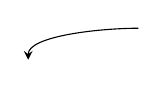
\begin{tikzpicture}[>=stealth]\draw[->] (1.4,0.4) .. controls (0.9,0.4) and (0,0.3) .. (0,0);\end{tikzpicture}}
(on n'a enlevé que les sommets et centres faces)

À cause de cet \deleted{de} isomorphisme, on fait \deleted{$\unsure{D_n}$} $D_{2n}$ opérer sur
$\Sigma_n^{\substack{*\\*}*}(\simeq\Sigma_{2n}^{\substack{*\\*}\cdot})$, on peut

\unsure{donc|dont}
}

\diagram{\begin{tikzcd}[ampersand replacement=\&,column sep=large,row sep=large]
 \& \begin{gathered}\Sigma_n^{\substack{*\\*}*}\\\simeq\Sigma_{2n}^{\substack{*\\*}\cdot}\end{gathered}
 \arrow[dl]\arrow[dr] \& \\
\Sigma_{2n}^{\substack{*\\*}\cdot}/D_{2n}^+\arrow[dd]
 \& \& \Sigma_n^{\substack{*\\*}*}/D_n^+\arrow[ll]\arrow[dl] \\
 \& \Sigma^{\substack{*\\*}*}/D_n\arrow[dl,bend left=12] \& \\
\Sigma_{2n}^{\substack{*\\*}\cdot}/D_{2n} \& \&
\end{tikzcd}}

% Curved guide from the central quotient toward the enclosed regrouping;
% it is separate from the quotient arrows.
\figure{\begin{tikzpicture}[>=stealth]\draw[->] (0,0) .. controls (0.8,0) and (1.4,0.2) .. (1.6,0.8);\end{tikzpicture}}

\diagram{\begin{tikzpicture}\node (d) at (0,0) {\begin{tikzcd}[ampersand replacement=\&,column sep=large,row sep=large]
 \& \Sigma_n^{\substack{*\\*}*}\simeq\Sigma_{2n}^{\substack{*\\*}\cdot}\arrow[d] \& \\
 \& \Sigma_n^{\substack{*\\*}*}/D_n^+\simeq\Sigma_1^{\substack{*\\*}*}\simeq\Sigma_2^{\substack{*\\*}\cdot}\arrow[dl]\arrow[dr] \& \\
\Sigma^{\substack{*\\*}\substack{*\\\unsure{*|\cdot}}}/D_{2n}^+\arrow[dr] \& \& \Sigma_n^{\substack{*\\*}*}/D_n\arrow[dl,dash] \\
 \& \Sigma_n^{\substack{*\\*}\cdot}/D_{2n} \&
\end{tikzcd}};\draw[rounded corners=22pt] (d.south west) rectangle (d.north east);\end{tikzpicture}}

\diagram{\begin{tikzcd}[ampersand replacement=\&]
\Sigma_n^{\substack{*\\*}\cdot}\arrow[r,"D_n^+"] \& \Sigma_1^{\substack{*\\*}\cdot}\simeq U_0^3
\end{tikzcd}}

Si on divise par $D_n$ tout entier, on trouve de la ramification sous les arêtes

\mspage{111}

\scanpage{113}

\figure{%
\begin{tikzpicture}[x=0.85cm,y=0.85cm,>=stealth]
\draw[thin] (0,0) ellipse (5.45 and 2.8);
\draw[thin] (-0.02,0.03) ellipse (5.48 and 2.82);
\draw[thin] (0,0) ellipse (5.02 and 2.17);
\draw[thin] (0,0) ellipse (4.45 and 1.56);
\draw[thick] (-4.11,-2.01) .. controls (-2.98,-2.56) and (-1.9,-2.66) .. (-0.8,-2.7);
\fill (-0.47,1.55) circle (0.05);\node at (-0.39,1.38) {$R_3$};
\draw[thin] (-0.48,1.55) ellipse (0.55 and 0.3);
\fill (-1.02,1.55) circle (0.025);\fill (0.08,1.55) circle (0.025);
\node at (-1.03,1.28) {$R_{3,\omega}$};\node at (0.36,1.27) {$R_{3,\omega'}$};
\draw[thin] (0.1,2.8) ellipse (0.63 and 0.16);
\draw[thin] (-0.1,2.16) ellipse (0.64 and 0.17);
\draw[thin] (-0.53,2.8) -- (-0.74,2.16);\draw[thin] (0.74,2.8) -- (0.54,2.16);
\draw[thin,<-] (0.1,2.8) -- (-0.1,2.16);
\draw[thin] (-0.53,2.8) .. controls (-0.75,2.7) and (-0.92,2.2) .. (-0.74,2.16);
\draw[thin,<-] (0.74,2.8) .. controls (0.9,2.6) and (0.67,2.23) .. (0.54,2.16);
\draw[thin,->] (-1.48,2.74) .. controls (-1.29,2.79) and (-1.08,2.84) .. (-0.91,2.8);
\draw[thin] (-1.52,2.78) .. controls (-1.25,2.89) and (-1.04,2.94) .. (-0.92,2.83);
\draw[thin] (-1.48,1.54)--(-1.43,1.59)--(-1.35,1.55);
\draw[thin] (-0.95,1.72)..controls (-0.8,1.9) and (-0.68,1.95)..(-0.62,1.87)--(-0.72,1.81);
\node at (0.11,3.07) {$\widetilde{R}_3$};\node at (-0.07,1.99) {$-\widetilde{R}_3$};
\node at (-0.72,3.04) {$R_3^{\omega'}$};\node at (0.96,3.03) {$R_3^{\omega'}$};
\node at (0.9,2.03) {$-R_3^{\omega'}$};
\draw[thin] (3.01,2.34) .. controls (3.02,2.1) and (2.75,1.78) .. (2.61,1.72);
\draw[thin] (3.01,2.34) -- (2.61,1.72);
\node at (3.23,2.57) {$Q_1^{\omega'}$};\node at (3.03,1.76) {$Q_1^{\omega^2}$};
\draw (2.3,1.17) ++(-0.045,-0.05) -- ++(0.09,0.1);\draw (2.3,1.17) ++(-0.04,0.05) -- ++(0.08,-0.1);
\node at (2.38,0.95) {$Q_1$};
\draw (-3.83,0.8) ++(-0.045,-0.05) -- ++(0.09,0.1);\draw (-3.83,0.8) ++(-0.04,0.05) -- ++(0.08,-0.1);
\node at (-3.69,0.59) {$Q_2$};
\draw[thin] (-5.08,1.01) ellipse (0.13 and 0.05);
\draw[thin] (-5.13,0.99) ellipse (0.12 and 0.07);
\draw[thin,black!55] (-0.165,-1.535)--(-0.075,-1.625);
\draw[thin,black!55] (-0.135,-1.635)..controls (-0.12,-1.59) and (-0.1,-1.56)..(-0.08,-1.545);
\draw[thin,black!45] (-0.09,-1.545)..controls (-0.05,-1.51) and (-0.085,-1.505)..(-0.1,-1.54)..controls (-0.13,-1.56) and (-0.12,-1.58)..(-0.085,-1.565);
\draw (0,-1.56) ++(-0.045,-0.06) -- ++(0.09,0.12);\draw (0,-1.56) ++(-0.04,0.06) -- ++(0.08,-0.12);
\node at (0.15,-1.78) {$Q_3$};
\draw[thick,->] (-0.08,-2.17) .. controls (-0.27,-2.29) and (-0.35,-2.69) .. (-0.32,-2.79);
\draw[thick,->] (-0.32,-2.79) .. controls (-0.12,-2.7) and (-0.04,-2.28) .. (-0.08,-2.17);
\draw[thick,->] (-0.2,-2.35)--(-0.26,-2.56);
\draw[thick,->] (-0.22,-2.62)--(-0.13,-2.4);
\draw[thin] (-0.07,-2.18)..controls (-0.05,-2.46) and (-0.21,-2.77)..(-0.3,-2.8);
\node at (0.35,-2.18) {$\overset{\unsure{\sim}}{Q}_3^{\omega'}$};
\node at (-0.03,-3.06) {$Q_3^\omega$};
\node[anchor=east] at (-0.23,-2.94) {$\scriptstyle\unsure{\deleted{\omega}|\sim}$};
\begin{scope}[shift={(-3.68,-1.05)}]
\fill (0,0) circle (0.045);\node at (0.18,-0.08) {$R_1$};
\draw[->] (0.33,0.42) .. controls (-0.02,0.61) and (-0.27,0.5) .. (-0.35,0.36);
\draw[->] (0.38,0.4) .. controls (0.62,0.24) and (0.61,0.09) .. (0.59,-0.03);
\draw[->,thick] (0.08,-0.4) .. controls (0.4,-0.53) and (0.49,-0.29) .. (0.52,-0.19);
\draw[->] (0.47,-0.26) .. controls (0.43,-0.37) and (0.34,-0.43) .. (0.23,-0.41);
\draw[->] (-0.4,-0.01) -- (-0.44,0.23);
\node at (-0.58,0.33) {$R_{1,\omega'}$};\node at (0.72,-0.21) {$R_{1,\omega}$};
\end{scope}
\begin{scope}[shift={(-4.7,-2.05)},rotate=-43]
\draw[thin] (0,0) ellipse (0.53 and 0.28);\draw[thin] (0,0.75) ellipse (0.53 and 0.26);
\draw[thin] (-0.53,0) -- (-0.53,0.75);\draw[thin] (0.53,0) -- (0.53,0.75);
\draw[<->,thick] (-0.5,0.06) .. controls (-0.8,-0.39) and (0.16,-0.45) .. (0.5,-0.05);
\draw[<->,thick] (-0.5,0.07) .. controls (-0.19,0.46) and (0.76,0.3) .. (0.53,-0.06);
\draw[<->,thick] (-0.5,0.77) .. controls (-0.7,0.31) and (0.14,0.32) .. (0.5,0.7);
\draw[->,thick] (0.5,0.7) .. controls (0.77,1.11) and (-0.17,1.19) .. (-0.5,0.77);
\draw[->] (-0.51,0.2) -- (-0.51,0.66);
\draw[->] (0.16,0.29)--(0.34,0.2);
\draw[->,thick] (0.12,1.03)--(0.34,0.94);
\node[rotate=43] at (-0.02,0.03) {$\widetilde{R}_1$};\node[rotate=43] at (0,0.77) {$-\widetilde{R}_1$};
\node[rotate=43] at (-0.74,0.05) {$R_1^{\omega'}$};\node[rotate=43] at (0.67,-0.18) {$R_1^\omega{}_{\deleted{\unsure{-}}}$};
\node[rotate=43] at (-0.61,1.04) {$-R_1^{\omega'}$};\node[rotate=43] at (0.82,0.73) {$-R_1^\omega$};
\end{scope}
\begin{scope}[shift={(3.16,-1.14)}]
\fill (0,0) circle (0.05);\node at (0.18,-0.13) {$R_2$};
\draw[->,thick] (0.37,0.29) .. controls (0.25,0.46) and (-0.21,0.39) .. (-0.36,0.22);
\draw[->,thick] (-0.38,-0.19) .. controls (0.1,-0.51) and (0.5,-0.18) .. (0.44,0.05);
\node at (-0.5,-0.23) {$R_{2,\omega'}$};\node at (0.66,0.12) {$R_{2,\omega}$};
\end{scope}
\begin{scope}[shift={(3.75,-2.04)},rotate=12]
\draw[thick] (0,0.4) ellipse (0.72 and 0.15);\draw[thick] (0.72,-0.45) arc (0:-180:0.72 and 0.15);
\draw[->,thick] (0.18,-0.30)..controls (-0.15,-0.28) and (-0.49,-0.32)..(-0.70,-0.44);
\draw[thick,line cap=round] (0.18,-0.30)--(0.18,-0.22);
\draw[thin,black!35] (0.18,-0.30)..controls (0.23,-0.30) and (0.28,-0.31)..(0.34,-0.32);
\draw[thick] (0.34,-0.32)..controls (0.54,-0.34) and (0.66,-0.38)..(0.72,-0.45);
\draw (-0.72,0.4) -- (-0.72,-0.45);\draw (0.72,0.4) -- (0.72,-0.45);
\draw[->,thick] (0.62,0.52) -- (-0.48,0.47);
\fill (0.015,0.54)--(0.035,0.66)--(0.10,0.55)--cycle;
\draw[thick,line cap=round] (-0.12,0.57)--(-0.10,0.60);\draw[<-,thick] (-0.6,0.29) -- (0.6,0.34);
\draw[->,thick] (0.6,0.25) -- (0.6,-0.37);\draw[->] (0.74,-0.34) -- (0.74,0.3);
\draw[->,thick] (-0.61,-0.34) -- (-0.61,0.28);
\draw[->,thick] (-0.78,0.26)..controls (-0.83,0) and (-0.82,-0.21)..(-0.75,-0.35);
\draw[->,thick] (-0.6,-0.58) -- (0.6,-0.49);
\draw[thick,line cap=round] (-0.64,0.16)--(-0.44,0.10);
\draw[thick,line cap=round] (-0.64,0.16)--(-0.65,0.20);
\draw[thin,black!40] (-0.44,0.10)--(-0.34,0.09);
\fill (-0.35,0.06)--(-0.36,0.09)--(-0.32,0.13)--(-0.21,0.13)--(-0.27,0.06)--cycle;
\node[rotate=-12] at (0,0.27) {$\widetilde{R}_2$};\node[rotate=-12] at (0,-0.59) {$-\widetilde{R}_2$};
\node[rotate=-12] at (-0.98,0.4) {$\widetilde{R}_2^{\omega'}$};
\node[rotate=-12] at (0.92,0.48) {$R_2^\omega$};
\node[rotate=-12] at (-0.88,-0.68) {$-R_2^{\omega'}$};
\node[rotate=-12] at (0.96,-0.43) {$R_2^\omega{}_{\deleted{\unsure{\omega}}}$};
\end{scope}
\end{tikzpicture}%
}

\figure{%
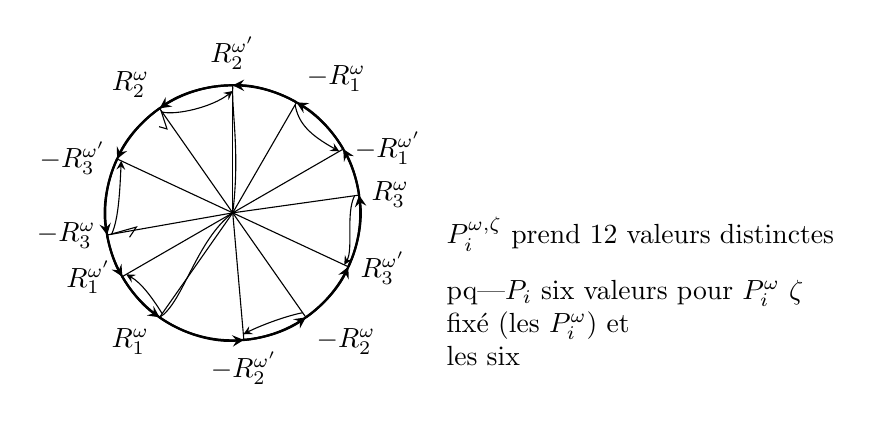
\begin{tikzpicture}[x=0.72cm,y=0.72cm,>=stealth]
\draw[thick] (0,0) circle (2.25);
\foreach \a in {90,125,60,30,8,-25,-55,-85,-125,-150,-170,155}{\draw[thin] (0,0)--(\a:2.25);}
\node[above] at (90:2.35) {$R_2^{\omega'}$};
\node[above left] at (125:2.27) {$R_2^\omega$};
\node[above right] at (60:2.27) {$-R_1^\omega$};
\node[right] at (30:2.29) {$-R_1^{\omega'}$};
\node[right] at (8:2.3) {$R_3^\omega$};
\node[right] at (-25:2.3) {$R_3^{\omega'}$};
\node[below right] at (-55:2.28) {$-R_2^\omega$};
\node[below] at (-85:2.28) {$-R_2^{\omega'}$};
\node[below left] at (-125:2.28) {$R_1^\omega$};
\node[left] at (-150:2.28) {$R_1^{\omega'}$};
\node[left] at (-170:2.28) {$-R_3^\omega$};
\node[left] at (155:2.28) {$-R_3^{\omega'}$};
\draw[->,thick] (90:2.25) arc (90:125:2.25);
\draw[->] (125:2.17) .. controls (-1.0,1.72) and (-0.37,1.86) .. (90:2.15);
\draw[->,thick] (125:2.25) arc (125:155:2.25);
\draw[->,thick] (60:2.25) arc (60:90:2.25);
\draw[->,thick] (8:2.25) arc (8:30:2.25);
\draw[->,thick] (-55:2.25) arc (-55:-25:2.25);
\draw[->,thick] (-170:2.25) arc (-170:-150:2.25);
\draw[->] (60:2.2) .. controls (1.16,1.57) and (1.37,1.37) .. (30:2.17);
\draw[->,thick] (30:2.25) arc (30:60:2.25);
\draw[->,thick] (-25:2.25) arc (-25:8:2.25);
\draw[->] (8:2.17) .. controls (1.99,-0.01) and (2.13,-0.64) .. (-25:2.17);
\draw[->,thick] (-85:2.25) arc (-85:-55:2.25);
\draw[->] (-55:2.15) .. controls (0.89,-1.83) and (0.44,-2.01) .. (-85:2.15);
\draw[->,thick] (-125:2.25) arc (-125:-85:2.25);
\draw[->,thick] (-150:2.25) arc (-150:-125:2.25);
\draw[->] (-125:2.17) .. controls (-1.43,-1.48) and (-1.62,-1.23) .. (-150:2.17);
\draw[->,thick] (155:2.25) arc (155:190:2.25);
\draw[->] (-170:2.17) .. controls (-2.01,-0.11) and (-1.99,0.43) .. (155:2.17);
\draw[thin] (90:2.22)..controls (-0.02,1.79) and (0.13,1.05)..(0,0);
\draw[thin] (0,0)..controls (-0.65,-0.49) and (-0.88,-1.6)..(-125:2.25);
\draw[thin] (-170:2.2)--(-1.7,-0.25)--(-1.82,-0.43);
\draw[thin] (125:2.21)--(-1.16,1.48)--(-1.3,1.52);
\node[anchor=north west,align=left,text width=5.0cm] at (3.6,0.1) {%
$P_i^{\omega,\zeta}$ prend $12$ valeurs distinctes\\[0.8em]
\unsure{pq|$P_i$} six valeurs pour \deleted{$P_i^{\unsure{\omega}}$} $\zeta$\\
fixé (les $P_i^\omega$) et\\
les six};
\end{tikzpicture}%
}

\figure{%
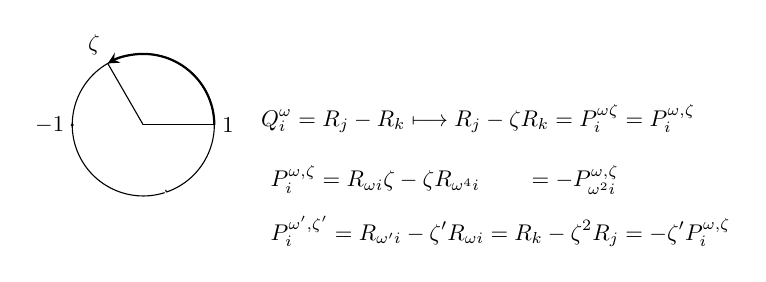
\begin{tikzpicture}[>=stealth,scale=0.82,transform shape]
\draw (-71:1.1) arc (-71:287.5:1.1);
\draw (-71:1.1)--++(-0.012,0.035);
\draw (0,0)--(1.1,0);\draw (0,0)--(120:1.1);
\draw[->,thick] (1.1,0) arc (0:120:1.1);
\fill (-1.1,0) circle (0.025);\node[left] at (-1.1,0) {$-1$};
\node[right] at (1.1,0) {$1$};\node[above left] at (120:1.1) {$\zeta$};
\node[anchor=west] at (1.7,0.1) {$\displaystyle
Q_i^\omega=R_j-R_k\longmapsto R_j-\zeta R_k
=P_i^{\omega\deleted{\unsure{\zeta}}}=P_i^{\omega,\zeta}$};
\node[anchor=west] at (1.85,-0.85) {$\displaystyle
P_i^{\omega,\zeta}=R_{\omega i}\deleted{\zeta}-\zeta R_{\omega^4i}
\qquad=-P_{\omega^2i}^{\omega,\zeta}$};
\node[anchor=west] at (1.85,-1.65) {$\displaystyle
P_i^{\omega',\zeta'}=R_{\omega'i}-\zeta'R_{\omega i}
=R_k-\zeta^2R_j=-\zeta'P_i^{\omega,\zeta}$};
\end{tikzpicture}%
}

\mspage{112}

\scanpage{114}
\mspage{1}

Carte $X$ (pas orientée)\inserted{finie}, $\mathcal R$ ens. des repères,
$S=\underset{\text{sommets}}{S_0}\amalg\underset{\text{arêtes}}{S_1}\amalg\underset{\text{faces}}{S_\infty}$
l'ens de ces facettes, identifiées à \deleted{\unsure{aux}} leurs centres, donc si on désigne par $X$ aussi la \unsure{surface} topologique sous-jacente : $X$, on a
\[
 S=S_0\amalg S_1\amalg S_\infty\subset X
\]

si $\varphi\in S$, on désigne par $R_\varphi$ le sommet associé. On identifie un $r=(s,a,f)\in\mathcal R$ à la région triangulaire correspondante (c'est un triangle de la subdivision barycentrique), de sommets $R_s,R_a,R_f$, d'indices respectifs $0,1,\infty$. On oriente ce triangle dans le sens $0,1,\infty$ (orientation du repère). Les régions ``adjacentes'' sont $\tau_0(r),\tau_1(r),\tau_\infty(r)$, opposées respectivement aux sommets de type $0,1,\infty$ de $r$. Notons
\[
 (1)\quad
 \left\{\begin{aligned}
 \tau_1(\tau_0(r))&=\rho_\infty(r)\\
 \tau_0(\tau_1(r))&=\rho_\infty^{-1}(r)
 \end{aligned}\right.
 \qquad\text{(face conservée)}
\]
déduits de $r$ par ``rotation'' \inserted{d'un cran} autour du sommet du type $\infty$ resp. $0$, dans le sens \deleted{indiqué} de l'orientation définie par $r$ resp. dans le sens opposé. On a de $=$

\figure{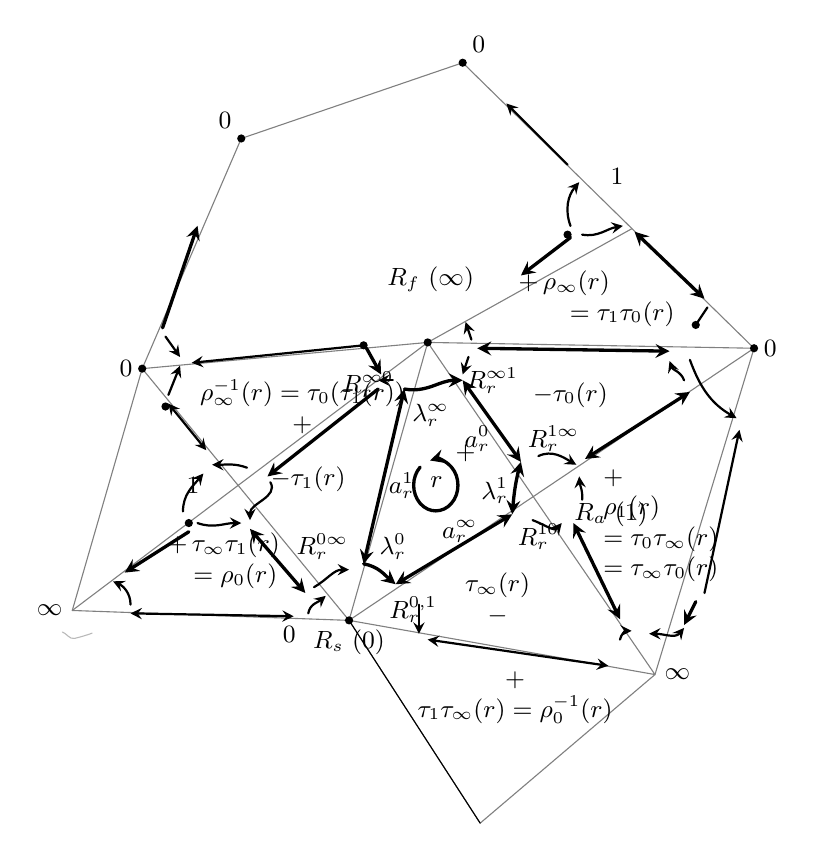
\begin{tikzpicture}[scale=.74,>=stealth,every node/.style={font=\small},line cap=round,line join=round]
\coordinate (T) at (7.5,-.6);
\coordinate (TL) at (3.7,-1.9);
\coordinate (L) at (2,-5.85);
\coordinate (LL) at (.8,-10);
\coordinate (F) at (6.9,-5.4);
\coordinate (S) at (5.55,-10.17);
\coordinate (A) at (9.5,-7.5);
\coordinate (TR) at (10.4,-3.45);
\coordinate (R) at (12.5,-5.5);
\coordinate (BR) at (10.8,-11.1);
\coordinate (B) at (7.8,-13.65);
\coordinate (AL) at (3.15,-7.5);
\draw[thin,gray] (TL)--(T)--(R)--(BR)--(B)--(S)--(LL)--(L)--cycle;
\draw[thin,gray] (L)--(S) (LL)--(F)--(R) (F)--(TR) (F)--(S) (F)--(BR) (S)--(R) (S)--(BR);
\draw[thin,gray] (L)--(F);
\draw[thin] (S)--(B);
% Detached pale trace below the LL--S baseline; its role is unresolved.
\draw[thin,gray,opacity=.55] (.63,-10.37)
 .. controls (.70,-10.39) and (.75,-10.50) .. (.84,-10.48)
 .. controls (.96,-10.45) and (1.06,-10.42) .. (1.14,-10.39);
\foreach \p in {T,TL,L,F,S,R} \fill (\p) circle (2pt);
\node[above right] at (T) {$0$};
\node[above left] at (TL) {$0$};
\node[left] at (L) {$0$};
\node[left] at (LL) {$\infty$};
\node[right] at (R) {$0$};
\node[right] at (BR) {$\infty$};
\node[below] at (S) {$R_s\ (0)$};
\node[above] at (6.95,-4.7) {$R_f\ (\infty)$};
\node[right] at (9.25,-8.35) {$R_a\ (1)$};
\node[above] at (10.15,-2.85) {$1$};
\node[left] at (3.15,-7.85) {$1$};
\node[below left] at (4.8,-10.1) {$0$};
\draw[->,very thick] (2.35,-5.15)--(2.95,-3.4);
\draw[->,thick] (9.3,-2.35)--(8.25,-1.3);
\draw[<->,very thick] (10.45,-3.5)--(11.65,-4.65);
\draw[->,very thick] (9.35,-3.6)--(8.5,-4.25);
\draw[->,thick] (9.35,-3.4) to[out=110,in=230] (9.5,-2.65);
\draw[->,thick] (9.55,-3.55) to[out=-10,in=190] (10.25,-3.4);
\fill (9.3,-3.55) circle (2pt);
\fill (11.5,-5.1) circle (2pt);
\draw[thick] (11.7,-4.8)--(11.5,-5.1);
\draw[->,thick] (11.4,-5.7) to[out=-70,in=150] (12.2,-6.7);
\draw[->,thick] (11.65,-9.7)--(12.25,-6.9);
\draw[<->,very thick] (9.4,-8.5)--(10.2,-10.15);
\draw[->,thick] (10.2,-10.5) to[out=80,in=180] (10.4,-10.35);
\draw[<->,thick] (11.3,-10.3) to[out=-130,in=0] (10.7,-10.4);
\draw[->,very thick] (11.5,-9.85)--(11.3,-10.25);
\draw[<->,thick] (6.9,-10.5)--(10,-10.95);
\draw[->,thick] (6.75,-9.9)--(6.75,-10.4);
\draw[<->,thick] (1.8,-10.05)--(4.6,-10.1);
\draw[->,thick] (1.8,-9.9) to[out=90,in=-25] (1.5,-9.5);
\draw[->,very thick] (2.8,-8.65)--(1.7,-9.35);
\fill (2.8,-8.5) circle (2pt);
\draw[->,thick] (2.7,-8.3) to[out=90,in=230] (3.05,-7.65);
\draw[->,thick] (2.95,-8.5) to[out=-20,in=180] (3.7,-8.5);
\draw[->,thick] (4.2,-7.8) to[out=-60,in=90] (3.85,-8.45);
\draw[->,thick] (3.8,-7.55) to[out=160,in=0] (3.2,-7.5);
\draw[<->,very thick] (3.85,-8.6)--(4.8,-9.7);
\draw[->,thick] (4.85,-10.05) to[out=80,in=-140] (5.15,-9.75);
\draw[->,thick] (4.95,-9.6) to[out=30,in=180] (5.55,-9.3);
\draw[<->,thick] (2.45,-6.45)--(3.1,-7.25);
\fill (2.4,-6.5) circle (2pt);
\draw[->,thick] (2.45,-6.3)--(2.65,-5.8);
\draw[->,thick] (2.4,-5.3)--(2.65,-5.65);
\draw[<-,thick] (2.85,-5.75)--(5.8,-5.45);
\fill (5.8,-5.45) circle (2pt);
\node[inner sep=0pt,font=\tiny,rotate=6] at (5.8,-5.45) {$\unsure{\blacktriangleright}$};
\draw[->,very thick] (5.85,-5.5)--(6.1,-5.95);
\draw[->,thick] (6.3,-6.05)--(6.05,-6.05);
\draw[->,very thick] (6.05,-6.2)--(4.15,-7.7);
\draw[<->,very thick] (7.75,-5.5)--(11.05,-5.55);
\draw[->,thick] (7.65,-5.35)--(7.55,-5.05);
\draw[->,thick] (7.6,-5.65)--(7.5,-5.95);
\draw[<->,very thick] (9.6,-7.4)--(11.4,-6.25);
\draw[->,thick] (11.3,-6.05) to[out=110,in=-70] (11.05,-5.72);
\draw[->,thick] (8.8,-7.35) to[out=25,in=150] (9.45,-7.5);
\draw[->,thick] (8.7,-8.45) to[out=-20,in=230] (9.2,-8.5);
\draw[->,thick] (9.55,-8.1) to[out=85,in=-85] (9.5,-7.7);
\coordinate (F0) at (6.5,-6.2);
\coordinate (F1) at (7.5,-6.05);
\coordinate (Ainf) at (8.5,-7.45);
\coordinate (A0) at (8.35,-8.35);
\coordinate (S1) at (6.35,-9.55);
\coordinate (Sinf) at (5.8,-9.2);
\draw[<->,very thick] (Sinf)--(F0);
\draw[->,very thick] (F0) to[out=-10,in=180] (F1);
\draw[<->,very thick] (F1)--(Ainf);
\draw[<->,very thick] (Ainf) to[out=-105,in=85] (A0);
\draw[<->,very thick] (A0)--(S1);
\draw[->,very thick] (Sinf) to[out=-10,in=140] (S1);
\draw[->,very thick] (6.77,-7.54) arc[start angle=135,end angle=465,x radius=.38,y radius=.44];
\node at (7.05,-7.8) {$r$};
\node at (7.55,-7.3) {$+$};
\node at (6.45,-7.85) {$a_r^1$};
\node at (7.75,-7.05) {$a_r^0$};
\node at (7.45,-8.65) {$a_r^\infty$};
\node at (6.95,-6.65) {$\lambda_r^\infty$};
\node at (8.05,-7.95) {$\lambda_r^1$};
\node at (6.3,-8.9) {$\lambda_r^0$};
\node[anchor=east] at (6.48,-6.12) {$R_r^{\infty 0}$};
\node[anchor=west] at (7.4,-6.05) {$\unsure{R_r^{\infty 1}}$};
\node[anchor=west] at (8.45,-7.05) {$R_r^{1\infty}$};
\node[anchor=north] at (8.8,-8.35) {$R_r^{10}$};
\node[anchor=east] at (5.7,-8.9) {$R_r^{0\infty}$};
\node[anchor=north] at (6.65,-9.6) {$R_r^{0,1}$};
\node at (4.85,-7.75) {$-\tau_1(r)$};
\node at (9.35,-6.3) {$-\tau_0(r)$};
\node[align=center] at (8.1,-9.8) {$\tau_\infty(r)$\\$-$};
\node[align=center] at (4.75,-6.5) {$\rho_\infty^{-1}(r)=\tau_0(\tau_1(r)\unsure{)}$\\$+$};
\node[align=left] at (9.8,-4.65) {$+\,\rho_\infty(r)$\\$\qquad=\tau_1\tau_0(r)$};
\node[align=left] at (3.4,-9.15) {$+\,\tau_\infty\tau_1(r)$\\$\quad=\rho_0(r)$};
\node[align=center] at (8.4,-11.5) {$+$\\$\tau_1\tau_\infty(r)=\rho_0^{-1}(r)$};
\node[align=left] at (10.9,-8.55) {$+$\\$\rho_1(r)$\\$=\tau_0\tau_\infty(r)$\\$=\tau_\infty\tau_0(r)$};
\end{tikzpicture}}

\[
 (2)\quad
 \left\{\begin{aligned}
 \tau_\infty\tau_1(r)&=\rho_0(r)\\
 \tau_1\tau_\infty(r)&=\rho_0^{-1}(r)
 \end{aligned}\right.
 \qquad\text{(sommet conservé)}
\]
où $\rho_0$ est la rotation \inserted{d'un cran} autour des sommets de type $0$, dans le sens indiqué par l'orientation choisie pour $r$. Enfin
\[
 (3)\qquad\tau_0\tau_\infty(r)=\tau_\infty\tau_0(r)\overset{\mathrm{def}}=\rho_1(r)
\]

[ Pour mémoire, les relations dans le groupe cartographique
\[
 (4)\qquad\tau_0^2\mathrel{\unsure{\begin{tikzpicture}[baseline=-.35ex,line cap=round,line join=round]
\draw[line width=.4pt] (0,.09)
 .. controls (.07,.11) and (.15,.095) .. (.18,.065)
 .. controls (.20,.02) and (.19,-.02) .. (.17,-.035)
 -- (.035,-.055);
\end{tikzpicture}}}\tau_1^2=\tau_\infty^2=(\tau_0\tau_\infty)^2=1
\]
\[
 (5)\quad
 \left\{\begin{aligned}
 \rho_\infty&=\tau_1\tau_0\\
 \rho_0&=\tau_\infty\tau_1\\
 \rho_1&=\tau_0\tau_\infty
 \end{aligned}\right.
 \qquad\rho_\infty\rho_1\rho_0\deleted{\unsure{\rho_\infty}}=1
 \qquad\text{]}
\]
\mspage{113}

\scanpage{115}
\mspage{2}

On introduit des sommets
\[
(6)\qquad R_r^{i,j}\qquad r\in\mathcal{R},\quad (i,j)\in\operatorname{Rep}\{0,1,\infty\}\quad\text{i.e. }i,j\in\{0,1,\infty\},\ i\ne j
\]
comme indi\uline{qués, satisfaisant} aux seules relations
\[
(7)\qquad
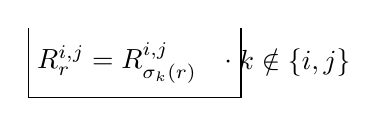
\begin{tikzpicture}[baseline=(relation.base)]
  \node[inner xsep=3pt,inner ysep=5pt] (relation)
    {$R_r^{i,j}=R_{\sigma_k(r)}^{i,j}\quad\cdot$};
  \draw[line width=.45pt] (relation.north west) -- (relation.south west)
    -- (relation.south east) -- (relation.north east);
  \node[anchor=west,inner sep=0pt,xshift=-1pt] at (relation.east)
    {$k\notin\{i,j\}$};
\end{tikzpicture}
\]
On dit que $R_r^{ij}$ est ``proche'' du
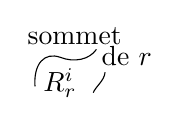
\begin{tikzpicture}[baseline=(baseR.base)]
  \node[anchor=base west,inner sep=0pt] (baseR) at (0,0) {$R_r^i$};
  \node[anchor=base west,inner sep=0pt] at (-.20,.59) {\inserted{sommet}};
  \node[anchor=base west,inner sep=0pt] at (.74,.33) {\inserted{de $r$}};
  \draw[line width=.4pt] (-.10,.06) .. controls (-.12,.35) and (.02,.50) .. (.22,.43)
    .. controls (.40,.36) and (.59,.40) .. (.68,.53);
  \draw[line width=.4pt] (.79,.24) .. controls (.78,.13) and (.67,.06) .. (.64,-.02);
\end{tikzpicture}
($=R_s,R_o,R_f$ suivant que $i=0,1,\infty$), il se trouve sur le côté
\deleted{\unsure{du plus proche}} \inserted{qui joint celui-ci}
\deleted{\illegible{1} \unsure{repère} opposé} au sommet de type $j$.

On introduit des arcs
\[
(8)\qquad \lambda_r^i:R_r^{i,i+1,}\longrightarrow R_r^{i,i+2}\qquad r\in\mathcal{R},\ i\in\{0,1,\infty\}
\]
\[
(9)\qquad a_r^i:R_r^{i\deleted{\unsure{+2|i+2}},i+1}\longrightarrow R_r^{i+1,i+2}\qquad r\in\mathcal{R},\ i\in\{0,1,\infty\}
\]
\margin{\uline{NB} On écrit pour simplifier $i+1$ au lieu du résultat de la permutation circulaire $(0,1,\infty)\longmapsto(1,\infty,0)$, i.e. on identifie $\{0,1,\infty\}$ à $\mathbb{Z}/3\mathbb{Z}\ldots$}

\deleted{qui}
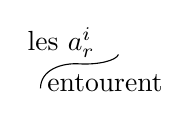
\begin{tikzpicture}[baseline=(entourent.base)]
  \node[anchor=base west,inner sep=0pt] (entourent) at (0,0) {entourent};
  \node[anchor=base west,inner sep=0pt] at (-.25,.52) {\inserted{les $a_r^i$}};
  \draw[line width=.4pt] (-.08,.04) .. controls (-.08,.27) and (.18,.37) .. (.43,.35)
    .. controls (.65,.34) and (.88,.39) .. (.91,.47);
\end{tikzpicture}
le drapeau repère $r$ en formant un contour fermé dans le sens
\deleted{\uline{opposé}} \inserted{de} l'orientation de $r$ ---
\deleted{par contre} \inserted{\unsure{de = désignent}} les $\lambda_r^i$
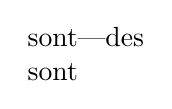
\begin{tikzpicture}[baseline=(oldverb.base)]
  \node[anchor=base west,inner sep=0pt] (oldverb) at (0,0) {\deleted{sont}};
  \node[anchor=base west,inner sep=0pt] at (0,.43) {\inserted{\unsure{sont|des}}};
\end{tikzpicture}
\deleted{\unsure{une}} portions d'arc tournant autour des sommets de $r$ de type $i$
dans le sens correspondant à l'orientation de $r$.
(Cela \deleted{\unsure{nous}} semble préférable à la convention de notation inverse).
On a les seules \deleted{identités} redondances
\[
(10)\qquad \boxed{a_r^i=a_{\tau_i(r)}^i}
\]
\margin{\begin{tabular}{@{}l@{}}
\uline{NB} On désigne\\
par les \deleted{\unsure{ces}} lettres\\
les flèches obtenues\\
après bouchage de\\
certains trous\\
si on bouche\\
$R_r^i$,
\end{tabular}}
\margin{\begin{tabular}{@{}l@{}}
(\uline{NB} si\\
les disques où\\
$\lambda_r^i$ devient $=1$)
\end{tabular}}

\deleted{On désigne}

\uline{NB} On supposera que la carte combinatoire se trouve réalisée par sa réalisation conforme canonique, qui est une surface $\unsure{\mathbb{C}|\mathcal{C}}$ analytique réelle donc $C^\infty$, dont on peut considérer son éclaté en les $R_\varphi$ $(\varphi\in S)$ et le découpe de l'éclaté, qui est une surface à bord analytique réelle (mais pas conforme) dont l'intérieur coïncide avec $X\setminus S$, on le note

\mspage{114}

\scanpage{116}

$\widetilde{X}^{\substack{*\\*}*\,\unsure{\vcenter{\hbox{\tikz[x=1mm,y=1mm]{\draw[line width=.4pt] (0,0)--(.04,.85);}}}}}$ ; (les trois $*$ signifient qu'on a enlevé \inserted{tous} les points de type $0,1,\infty$, disposés comme suit $\substack{\infty\\0}1$, on définirait de même $\widetilde{X}^{\substack{*\\\cdot}*}$, $\widetilde{X}^{\substack{\unsure{\cdot|*}\\*}*}$, $\widetilde{X}^{\substack{*\\*}\cdot}$, etc. \deleted{Donc} L'intérieur de cette surface à bord, savoir $X\setminus S=X\setminus\{R_\varphi\mid\varphi\in S\}$, est notée $X^{\substack{*\\*}*}$, on définit de $=$ $X^{\substack{*\\\cdot}*}$ etc. Les points $R_r^{ij}$ et les chemins précédents seront regardés, le plus commodément, comme points et chemins, (parfaitement canoniques, pas seulement des classes d'homotopie !) dans $\widetilde{X}^{\substack{*\\*}*}$. On notera que les $R_\varphi$ $(\varphi\in S)$ ne \uline{sont pas} dans $\widetilde{X}^{\substack{*\ *\\*}}$
\tikz[baseline=-.35ex]{
  \draw[line width=.4pt] (0,0)--(.55,.025);
  \node[inner sep=0pt] at (.08,-.18) {$\unsure{\vcenter{\hbox{\tikz[x=1mm,y=1mm,line width=.45pt]{
    \draw (.12,.72) .. controls (-.1,.54) and (.03,.14) .. (.38,.13)
      .. controls (.68,.11) and (.7,.48) .. (.45,.58)
      .. controls (.28,.64) and (.11,.46) .. (.2,.3);
    \draw (.4,.61)--(.77,.18)--(.6,-.03);
  }}}}$};
}
mais dans l'application $C^\infty$ (\unsure{et $=$|$\ne$} analytique réelle) canonique
\diagram{
$(11)\qquad$
\begin{tikzcd}[ampersand replacement=\&]
\widetilde{X}^{\substack{*\\*}*} \arrow[r] \& X
\end{tikzcd}
}
Le point $R_r^{ij}$ va sur $R_r^i=R_\varphi$, où $\varphi$ est le \deleted{point} \inserted{sommet} de type $i$ de $r$.

On a, dans $\Pi_1 X^{\substack{*\\*}*}$, la relation
\reversemarginpar
\margin{\vspace*{1.8\baselineskip}
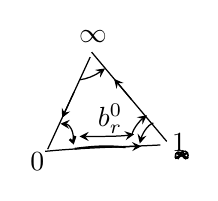
\begin{tikzpicture}[x=.9cm,y=.9cm,>=stealth,line width=.45pt]
  % Three separately drawn contours: small pen gaps at the apex and at 1.
  \draw (.02,.02)--(.62,1.32);
  \draw (.64,1.39)--(1.7,.13);
  \draw (-.015,-.01) .. controls (.54,.045) and (1.17,.055) .. (1.61,.08);
  \draw[line width=.7pt] (.4,.026) .. controls (.77,.075) and (.92,.063) .. (1.12,.048);
  \draw[->] (.392,.826)--(.224,.462);
  \draw[->] (1.2,.724)--(.958,1.012);
  \draw[->] (.91,.049)--(1.34,.061);
  % The three corner arcs, with the dense lower endpoint at 0 retained as ink.
  \draw[->] (.472,1.0) .. controls (.57,1.01) and (.68,1.055) .. (.83,1.16);
  \draw[<-] (.2,.38) .. controls (.34,.37) and (.41,.22) .. (.37,.13);
  \draw[line width=.85pt] (.33,.16)--(.38,.115)--(.41,.205);
  \draw[->] (1.51,.39) .. controls (1.42,.36) and (1.35,.22) .. (1.32,.1);
  % Opposed heads on the inner horizontal part, followed by the rising segment.
  \draw[<->] (.47,.2) .. controls (.8,.2) and (1.04,.2) .. (1.24,.23);
  \draw[->] (1.21,.23) .. controls (1.23,.32) and (1.33,.43) .. (1.42,.5);
  \node[below left,inner sep=1pt] at (.02,.02) {$0$};
  \node[right,inner sep=1pt] at (1.73,.12) {$1$};
  \node[above,inner sep=1pt] at (.66,1.48) {$\infty$};
  \node at (.9,.45) {$b_r^0$};
  % Dense overwritten or cancelled label below the live 1: identity/state doubtful.
  \node[inner sep=0pt] at (1.91,-.06) {$\unsure{\vcenter{\hbox{\tikz[x=1mm,y=1mm,line width=.55pt]{
    \draw (0,.35) .. controls (-.08,1.03) and (.64,1.25) .. (.91,.59)
      .. controls (1.08,.02) and (1.57,.01) .. (1.63,.55)
      .. controls (1.69,1.12) and (.91,1.35) .. (.61,.72)
      .. controls (.38,.26) and (.15,.02) .. (0,.35);
    \draw[line width=.8pt] (-.04,.21)--(1.52,.85);
    \draw[line width=.7pt] (.12,.85)--(1.66,.2);
    \draw (.31,.09)--(.94,1.05)--(1.38,.08);
  }}}}$};
\end{tikzpicture}}
\normalmarginpar
\[
(12)\qquad
\begin{tikzpicture}[baseline=(eq116.base),line width=.4pt]
\node[inner sep=6pt] (eq116) {$\displaystyle
\underbrace{(\lambda_r^0)^{-1}a_r^1}_{\underset{=}{\text{def}}\ b_r^\infty}
\underbrace{(\lambda_r^\infty)^{-1}a_r^0}_{b_r^1}
\underbrace{(\lambda_r^1)^{-1}a_r^\infty}_{b_r^0}=1
$};
% Four independent pen strokes; all four corners remain open.
\draw ([xshift=-1pt,yshift=-1pt]eq116.north west)
  -- ([xshift=-3pt,yshift=3pt]eq116.north east);
\draw ([xshift=0pt,yshift=-3pt]eq116.north east)
  -- ([xshift=3pt,yshift=3pt]eq116.south east);
\draw ([xshift=2pt,yshift=-2pt]eq116.south west)
  -- ([xshift=3pt,yshift=0pt]eq116.south east);
\draw ([xshift=-1pt,yshift=-5pt]eq116.north west)
  -- ([xshift=0pt,yshift=0pt]eq116.south west);
\end{tikzpicture}
\qquad\text{lacet en }R_r^{1\infty}
\]
Les sommets $R_r^{ij}$, les flèches $\lambda_r^i$ et $a_r^i$, et les relations $(10)$ $(17)$, forment une présentation du groupoïde $\Pi_1(\widetilde{X}^{\substack{*\\*}*},\unsure{\{|(}R_r^{i,j}))$.

\mspage{115}

\scanpage{117}
\mspage{3}

Les notations introduites sont telles qu'elles gardent un sens pour toute carte triangulaire ``polarisée'' de type $\{0,1,\infty\}$, sans que celle\deleted{\unsure{soit la|qui est la}} \inserted{-ci soit} nécessairement : la subdivision barycentrique d'une carte $X$, condition qui s'exprime par la 
\begin{tikzpicture}[baseline=(condition117.base)]
\node[anchor=base west,inner sep=0pt] (condition117) at (0,0) {\deleted{condition}};
\node[anchor=south west,inner sep=0pt] (derniere117)
  at ([xshift=-4pt,yshift=4pt]condition117.north west) {\inserted{dernière}};
\draw[line width=.35pt] ([xshift=-4pt,yshift=-2pt]condition117.west)
  .. controls ([xshift=-4pt,yshift=4pt]condition117.north west)
  and ([xshift=-1pt,yshift=-1pt]derniere117.south west) .. (derniere117.south west)
  -- ([xshift=-1pt,yshift=-1pt]derniere117.south east)
  .. controls ([xshift=2pt,yshift=-1pt]derniere117.south east)
  and ([xshift=3pt,yshift=0pt]derniere117.south east)
  .. ([xshift=2pt,yshift=2pt]derniere117.south east);
\end{tikzpicture} relation
\[
\deleted{\unsure{\tau_0\tau_\infty|\tau_0}}\qquad (\tau_0\tau_\infty)^2=1\qquad\text{i.e}\quad\rho_1^2=1
\]
dans $(4)$ (qu'on abandonne donc par la suite) et qui signifie aussi que les \deleted{points} \inserted{sommets} de type $1$ sont d'ordre réduit $2$ (d'ordre ordinaire $4$), ou encore que $\tau_0\tau_\infty(r)=\tau_\infty\tau_0(r)$ pour tout $r$. Dans le cas général, $\rho_1$ est donc une op. qui ne joue plus un rôle particulier p.r. à $\rho_0,\rho_\infty$ : c'est la rotation ``d'un cran'' de $r$ autour du sommet de type $1$, dans le \deleted{\unsure{demi-tour} \unsure{indiqué|défini}} \inserted{sens défini} par l'orientation de $r$.

On introduit
\[
(13)\qquad\left\{
\begin{aligned}
\Lambda_r^i&=(\lambda_{\tau_{i+1}}^i)^{-1}\lambda_r^i:R_r^{i,i+1}\mathrel{\tikz[baseline=-.5ex]{\draw[line width=.45pt] (0,0)--(.6,0)--(.6,.07);}} R_{\tau_{i+1}(r)}^{i,i+1}\\
\Lambda_r^{\prime i}&=\lambda_{\sigma_{i-1}(r)}^i(\lambda_r^i)^{-1}:R_r^{i,i-1}\mathrel{\tikz[baseline=-.5ex]{\draw[line width=.45pt] (0,0)--(.6,0)--(.6,.07);}} R_{\tau_{i-1}(r)}^{i-1}
\end{aligned}\right.
\]
rotation d'un double cran'' autour du sommet de type $i$ de $r$, à partir du sommet proche de type 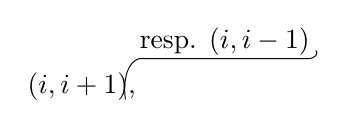
\begin{tikzpicture}[baseline=(type117.base)]
\node[anchor=base west,inner sep=0pt] (type117) at (0,0) {$(i,i+1)$,};
\node[anchor=south west,inner sep=0pt] (resptype117)
  at ([xshift=1pt,yshift=6pt]type117.north east) {\inserted{resp. $(i,i-1)$}};
\draw[line width=.35pt] ([xshift=-4pt,yshift=-2pt]type117.base east)
  .. controls ([xshift=-5pt,yshift=3pt]type117.east)
  and ([xshift=-4pt,yshift=-2pt]resptype117.south west)
  .. ([xshift=0pt,yshift=-1pt]resptype117.south west)
  -- ([xshift=-1pt,yshift=-1pt]resptype117.south east)
  .. controls ([xshift=2pt,yshift=-1pt]resptype117.south east)
  and ([xshift=3pt,yshift=1pt]resptype117.south east)
  .. ([xshift=2pt,yshift=2pt]resptype117.south east);
\end{tikzpicture} dans le sens de rotation donné par l'orientation de 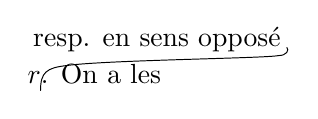
\begin{tikzpicture}[baseline=(orientation117.base)]
\node[anchor=base west,inner sep=0pt] (orientation117) at (0,0) {$r$. On a les};
\node[anchor=south west,inner sep=0pt] (respsens117)
  at ([xshift=2pt,yshift=4pt]orientation117.north west) {\inserted{resp. en sens opposé}};
\draw[line width=.35pt] (.17,-.09)
  .. controls (.17,.15) and (.25,.20) .. (.50,.23)
  .. controls (1.0,.30) and ([xshift=-6pt,yshift=-2pt]respsens117.south east)
  .. ([xshift=-1pt,yshift=-1pt]respsens117.south east)
  .. controls ([xshift=2pt,yshift=-1pt]respsens117.south east)
  and ([xshift=3pt,yshift=1pt]respsens117.south east)
  .. ([xshift=2pt,yshift=2pt]respsens117.south east);
\end{tikzpicture} relations

\figure{
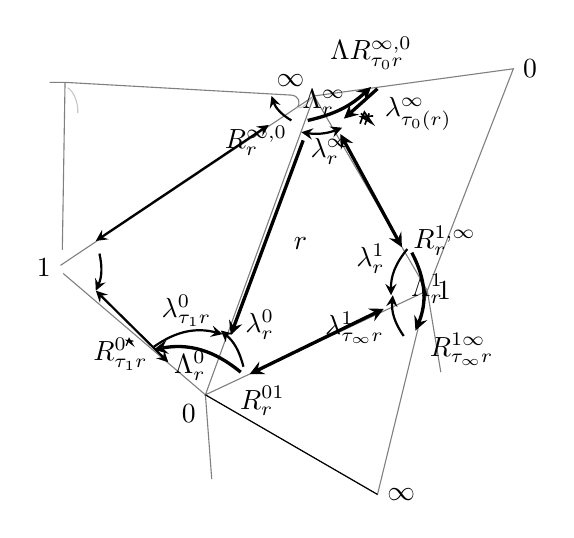
\begin{tikzpicture}[scale=1.15,>=stealth]
\coordinate (A) at (1.75,0.95);\coordinate (B) at (4.2,2.1);\coordinate (C) at (2.95,4.25);
\coordinate (D) at (0.15,2.35);\coordinate (E) at (5.15,4.55);\coordinate (F) at (3.65,-0.15);\coordinate (G) at (0.2,4.4);
% Pencil framework: separate tips at the outer 1 and literal local pen details.
\draw[gray] (C)--(E)--(B)--(F)--(A);
\draw[gray] (A)--(B)--(C)--cycle (A)--(1.82,0.02) (B)--(4.35,1.2);
\draw[gray] (G)--(.17,2.55);
\draw[gray] (.15,2.38)--(C);
\draw[gray] (.18,2.29)--(A);
\draw[gray] (G)--(.03,4.4);
\draw[gray!45,thin] (.23,4.34)
  .. controls (.29,4.31) and (.35,4.18) .. (.34,4.06);
% The faint intervening contour does not settle continuity at this junction.
\draw[gray] (G)--(2.70,4.26)
  .. controls (2.78,4.25) and (2.81,4.18) .. (2.76,4.12);
\draw[gray!45,thin] (2.76,4.12)
  .. controls (2.83,4.10) and (2.88,4.19) .. (C);
\draw[thin] (A)--(F);
\draw[very thick,->] (2.83,3.76)--(2.03,1.61);
\draw[very thick,<->] (2.24,1.18)--(3.72,1.9);
\draw[very thick,<->] (3.92,2.58)--(3.24,3.83);
\draw[thick,<->] (0.54,2.65)--(2.45,3.93);
\draw[thick,->] (0.58,2.51) to[bend left=18] (0.54,2.10);
\draw[thick,<->] (0.54,2.10)--(1.34,1.31);
\draw[thick,->] (2.17,1.26) to[bend right=18] (1.92,1.66);
\draw[thick,->] (1.18,1.48) to[bend left=25] (1.94,1.62);
\draw[very thick,->] (2.14,1.20) to[bend right=25] (1.18,1.45);
\draw[thick,->] (3.98,2.56) to[bend right=20] (3.80,2.05);
\node[inner sep=0pt,font=\tiny,rotate=-20] at (3.98,2.56) {$\unsure{\blacktriangle}$};
\draw[thick,->] (3.94,1.60) to[bend left=20] (3.82,2.05);
\draw[very thick,->] (4.03,2.52) to[bend left=25] (4.07,1.66);
\draw[thick,<->] (2.81,3.85) to[bend right=15] (3.26,3.90);
\draw[thick,->] (2.70,3.98) to[bend left=20] (2.48,4.25);
\draw[very thick,->] (2.88,3.98) to[bend right=15] (3.58,4.35);
\draw[very thick,->] (3.65,4.33)--(3.28,4.00);
\node[below left] at (A) {$0$};\node[right] at (B) {$1$};\node[above left] at (C) {$\infty$};
\node[left] at (D) {$1$};\node[right] at (E) {$0$};\node[right] at (F) {$\infty$};\node at (2.8,2.62) {$r$};
\node[below] at (2.38,1.15) {$R_r^{01}$};
\node[left] at (1.22,1.40) {$R_{\tau_1r}^{0\unsure{\tikz[x=.045cm,y=.045cm,baseline=-.4ex]{\draw[line width=.45pt] (0,0)--(.8,2)--(1.8,.3)--(.2,1.5)--(2,1.3);}}}$};
\node at (1.54,1.88) {$\lambda_{\tau_1r}^0$};\node at (1.58,1.27) {$\Lambda_r^0$};\node at (2.35,1.72) {$\lambda_r^0$};
\node[right] at (3.94,2.65) {$R_r^{1,\infty}$};\node[right] at (4.12,1.45) {$R_{\tau_\infty r}^{1\infty}$};
\node[left] at (3.84,2.45) {$\lambda_r^1$};\node[left] at (3.83,1.69) {$\lambda_{\tau_\infty r}^1$};\node at (4.20,2.12) {$\Lambda_r^1$};
\node[left] at (2.76,3.76) {$R_r^{\infty,0}$};\node[above] at (3.58,4.44) {$\deleted{\unsure{\Lambda}}R_{\tau_0r}^{\infty,0}$};
\node at (3.13,3.64) {$\lambda_r^\infty$};\node at (4.10,4.05) {$\lambda_{\tau_0(r)}^\infty$};\node at (3.06,4.18) {$\Lambda_r^\infty$};
\node[inner sep=0pt] at (3.53,3.98) {$\unsure{\tikz[x=.055cm,y=.055cm,baseline=-.5ex]{\draw[line width=.6pt] (0,0)--(1,2.7)--(2.8,.1)--(.3,1.6)--(3,1.8);\draw[line width=.6pt] (.2,2.4)--(2.5,.2) (1.1,-.2)--(2.1,2.4);}}$};
\end{tikzpicture}
}
\[
(14)\qquad 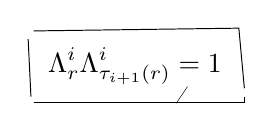
\begin{tikzpicture}[baseline=(eq14a.base)]
\node[inner sep=5pt] (eq14a) {$\displaystyle \Lambda_r^i\Lambda_{\tau_{i+1}(r)}^i=1$};
\draw[line width=.35pt] ([xshift=0pt,yshift=1pt]eq14a.north west)
  -- ([xshift=1pt,yshift=2pt]eq14a.north east)
  -- ([xshift=3pt,yshift=4pt]eq14a.south east);
\draw[line width=.35pt] ([xshift=-2pt,yshift=-2pt]eq14a.north west)
  -- ([xshift=-1pt,yshift=1pt]eq14a.south west);
\draw[line width=.35pt] ([xshift=0pt,yshift=-1pt]eq14a.south west)
  -- ([xshift=3pt,yshift=-1pt]eq14a.south east)
  -- ([xshift=3pt,yshift=1pt]eq14a.south east);
% Fine source trace; its origin and function remain uncertain.
\draw[line width=.18pt] ([xshift=15pt,yshift=-1.4pt]eq14a.south)
  -- ([xshift=19pt,yshift=4.6pt]eq14a.south);
\end{tikzpicture}\qquad
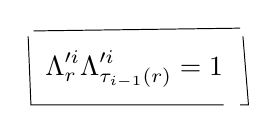
\begin{tikzpicture}[baseline=(eq14b.base)]
\node[inner sep=5pt] (eq14b) {$\displaystyle \Lambda_r^{\prime i}\Lambda_{\tau_{i-1}(r)}^{\prime i}=1$};
\draw[line width=.35pt] ([xshift=1pt,yshift=2pt]eq14b.north west)
  -- ([xshift=1pt,yshift=3pt]eq14b.north east);
\draw[line width=.35pt] ([xshift=-1pt,yshift=0pt]eq14b.north west)
  -- ([xshift=0pt,yshift=-1pt]eq14b.south west)
  -- ([xshift=-5pt,yshift=-1pt]eq14b.south east);
\draw[line width=.35pt] ([xshift=2pt,yshift=0pt]eq14b.north east)
  -- ([xshift=4pt,yshift=-1pt]eq14b.south east)
  -- ([xshift=1pt,yshift=-1pt]eq14b.south east);
\end{tikzpicture}
\]

\mspage{116}

\scanpage{118}
\mspage{117}
\mspage{4}
\deleted{Soit} $i$

\deleted{L'introduction des $\Lambda_r^i$}

Fixons nous un indice dans $\{0,1,\infty\}$, disons $1$ (en pensant au cas où la triangulation est barycentrique, donc
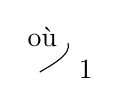
\begin{tikzpicture}[baseline=(one.base)]
\node[anchor=base west,inner sep=0pt] (one) at (.65,0) {$1$};
\node[anchor=base west,inner sep=0pt] at (0,.40) {\inserted{où}};
\draw[line width=.4pt] (.52,.45) .. controls (.57,.30) and (.29,.16) .. (.16,.08);
\end{tikzpicture}
joue un rôle particulier !). Nous pouvons éliminer les sommets $R_r^{ij}$ qui se trouvent sur des côtés de $r$ qui sont de type $1$, i.e. pour lesquels $i,j\ne1$, et l'arc $a_r^1$ qui les joint, en gardant les sommets
\[
(14)\qquad 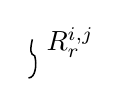
\begin{tikzpicture}[baseline=(rij.base)]
\node[inner sep=0pt] (rij) at (0,0) {$R_r^{i,j}$};
\draw[line width=.55pt] (-.48,.04) .. controls (-.51,-.09) and (-.51,-.15) .. (-.45,-.17)
  .. controls (-.42,-.28) and (-.44,-.45) .. (-.53,-.45);
\end{tikzpicture}\qquad
\left\{\begin{array}{l}
r\in\mathcal{R}\\
i\text{ ou }j\text{ est égal à }1\quad\text{i.e}\quad\{i,j\}\ne\{0,\infty\}
\end{array}\right.
\]
et les arcs
\[
(15)\qquad\left\{\begin{array}{ll}
\lambda_r^1&r\in\mathcal{R}\\
\Lambda_r^0,\Lambda_r^{\prime\infty}&r\in\mathcal{R},\quad\deleted{\unsure{i\in\{0,\infty\}}}\\
a_r^i&r\in\mathcal{R},\quad i\in\{0,\infty\}
\end{array}\right.
\]
\margin{$\Lambda_r^0\Lambda_{\tau_1r}^0=$}

avec comme relations les relations $(14)$ de
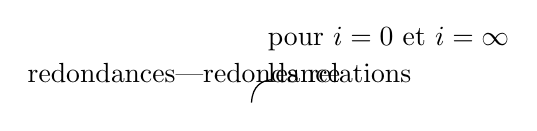
\begin{tikzpicture}[baseline=(red.base)]
\node[anchor=base west,inner sep=0pt] (red) at (0,0) {\unsure{redondances|redondance}};
\node[anchor=base west,inner sep=0pt] (oldwords) at (3.05,0) {\deleted{les relations}};
\node[anchor=base west,inner sep=0pt] at (3.05,.46) {\inserted{pour $i=0$ et $i=\infty$}};
\draw[line width=.45pt] (2.85,-.26) .. controls (2.86,-.04) and (2.99,.02) .. (3.10,.03);
\end{tikzpicture}
\deleted{du type $\unsure{\vcenter{\hbox{%
\begin{tikzpicture}[x=.55cm,y=.55cm]
\draw[line width=.45pt] (0.02,.65)..controls(0.03,.48)and(0.06,.30)..(0.015,.23)
 ..controls(-.02,.17)and(-.13,.20)..(-.12,.12)
 ..controls(-.10,.06)and(.07,.07)..(.08,-.04)
 ..controls(.10,-.12)and(.06,-.25)..(.13,-.26)--(.22,-.24);
\end{tikzpicture}}}}\Lambda_r^0=1$}

\figure{
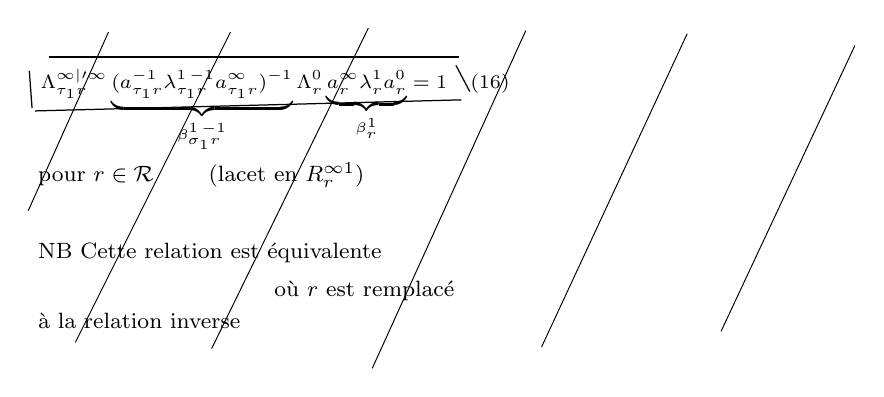
\begin{tikzpicture}[>=stealth]
\node[anchor=base west,inner sep=1pt,font=\scriptsize] (oldformula) at (0,0)
 {$\displaystyle \Lambda_{\unsure{\tau_1r}}^{\unsure{\infty|\prime\infty}}\underbrace{(a_{\tau_1r}^{-1}\lambda_{\tau_1r}^{1\,-1}a_{\tau_1r}^{\infty})^{-1}}_{\beta_{\sigma_1r}^{1\,-1}}\Lambda_r^0\underbrace{a_r^\infty\lambda_r^1a_r^0}_{\beta_r^1}=1$};
\node[anchor=base west,inner sep=0pt,font=\scriptsize] at ([xshift=7pt]oldformula.base east) {$(16)$};
\draw[line width=.45pt] ([xshift=4pt,yshift=3pt]oldformula.north west)
 -- ([xshift=3pt,yshift=3pt]oldformula.north east);
\draw[line width=.45pt] ([xshift=-3pt,yshift=-2pt]oldformula.north west)
 -- ([xshift=-2pt,yshift=-7pt]oldformula.base west);
\draw[line width=.45pt] ([xshift=-1pt,yshift=-8pt]oldformula.base west)
 -- ([xshift=4pt,yshift=-4pt]oldformula.base east);
\draw[line width=.45pt] ([xshift=2pt,yshift=0pt]oldformula.north east)
 -- ([xshift=7pt,yshift=-1pt]oldformula.base east);
\node[anchor=base west,inner sep=0pt,font=\footnotesize] at (0,-1.18)
 {pour $r\in\mathcal R$ \qquad (lacet en $R_r^{\infty1}$)};
\node[anchor=base west,inner sep=0pt,font=\footnotesize] at (0,-2.15)
 {\uline{NB} Cette relation est équivalente};
\node[anchor=base west,inner sep=0pt,font=\footnotesize] at (0,-3.05)
 {à la relation \deleted{\unsure{inverse}}};
\node[anchor=base west,inner sep=0pt,font=\footnotesize] at (3.00,-2.64)
 {\inserted{où $r$ est remplacé}};
% The six long cancellation strokes cross the formula and the prose together.
\draw[line width=.35pt] (.90,.72)--(-.12,-1.55);
\draw[line width=.35pt] (2.45,.72)--(.48,-3.22);
\draw[line width=.35pt] (4.20,.77)--(2.21,-3.30);
\draw[line width=.35pt] (6.20,.74)--(4.25,-3.55);
\draw[line width=.35pt] (8.25,.70)--(6.40,-3.28);
\draw[line width=.35pt] (10.38,.55)--(8.68,-3.08);
\end{tikzpicture}
}

\margin{pavage par des carrés ? (dont les sommets qui ne sont pas de type $1$, sont ``arrondis'', de façon à faire des hexagones évitant les trous}
\figure{
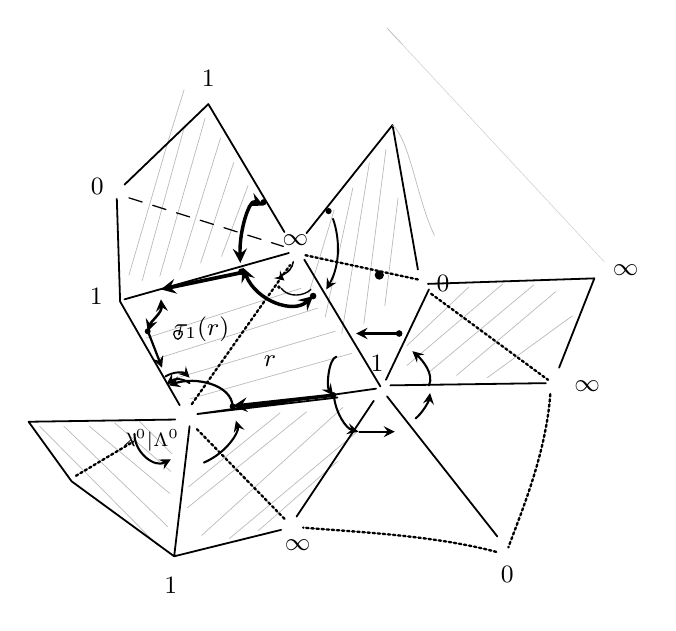
\begin{tikzpicture}[x=.014cm,y=-.014cm,>=stealth,line cap=round,line join=round]
\draw[gray!35,line width=.22pt] (595,1462)--(792,1674);
\draw[gray!50,line width=.22pt] (595,1462)--(609,1477);
% Light construction hatching: six local regions, with independently drawn strokes.
\draw[gray!55,line width=.25pt]
 (361,1686)--(397,1563)--(411,1518) (373,1691)--(412,1549) (389,1687)--(430,1544)
 (407,1681)--(444,1562) (426,1675)--(456,1584) (445,1669)--(469,1605);
\draw[gray!55,line width=.25pt]
 (524,1703)--(547,1627) (539,1724)--(564,1607) (554,1739)--(579,1584)
 (574,1730)--(594,1572) (593,1714)--(605,1616)
 (613,1750)--(669,1697) (613,1768)--(700,1694) (632,1775)--(728,1695)
 (658,1777)--(748,1701) (686,1779)--(763,1723)
 (377,1743)--(517,1698) (389,1761)--(532,1716) (402,1780)--(548,1737)
 (417,1798)--(563,1757)
 (414,1897)--(522,1810) (415,1878)--(498,1811) (427,1922)--(555,1806)
 (452,1925)--(568,1828) (478,1918)--(550,1855)
 (280,1823)--(387,1931) (302,1823)--(396,1914) (325,1823)--(398,1884)
 (348,1820)--(399,1864) (370,1818)--(400,1848);
% Solid edges stop separately around the punctured 0 and infinity corners.
\draw[line width=.65pt]
 (357,1604)--(433,1531)--(502,1647)
 (350,1617)--(353,1710)--(407,1804)
 (357,1708)--(506,1666)
 (520,1672)--(589,1787)
 (423,1812)--(585,1789)
 (416,1823)--(402,1941)
 (423,1812)--(550,1797)
 (522,1648)--(600,1550)--(623,1681)
 (632,1694)--(783,1689)--(751,1770)
 (633,1699)--(594,1781)
 (598,1786)--(739,1784)
 (595,1796)--(695,1923)
 (583,1800)--(513,1905)
 (499,1917)--(402,1941)--(309,1873)--(270,1819)--(403,1817);
\draw[gray!55,line width=.25pt] (600,1550)..controls(616,1564)and(622,1617)..(638,1650);
% The upper-left cross-edge uses long dashes, not dots.
\draw[dash pattern=on 5pt off 4pt,line width=.45pt] (361,1616)--(501,1660);
% The other cross-edges and outer continuation are dotted, with heavy round marks.
\draw[densely dotted,line width=.85pt]
 (521,1668)--(623,1690) (635,1703)--(741,1781)
 (743,1794)..controls(739,1850)and(715,1905)..(705,1933)
 (694,1937)..controls(638,1922)and(568,1919)..(519,1915)
 (502,1907)--(421,1824) (418,1803)--(507,1677)
 (313,1868)--(365,1837);
% Marked endpoints and thick directional paths at the top/left infinity corner.
\fill (483,1620) circle[radius=2.8];
\fill (542,1628) circle[radius=2.8];
\fill (588,1686) circle[radius=4.2];
\fill (463,1683) circle[radius=3.0];
\fill (528,1705) circle[radius=3.0];
\draw[line width=1.35pt,<-] (390,1699)--(462,1684);
\draw[line width=1.25pt,<->] (483,1623)..controls(470,1617)and(461,1646)..(462,1675);
\draw[line width=1.25pt,<->] (464,1679)..controls(477,1710)and(510,1721)..(528,1705);
\draw[line width=.7pt,->] (546,1635)..controls(552,1652)and(553,1676)..(540,1699);
\draw[line width=.55pt,->] (510,1674)..controls(508,1686)and(496,1686)..(502,1691);
\fill (497,1697) circle[radius=1.8];
\draw[line width=.5pt] (499,1698)..controls(506,1707)and(520,1705)..(526,1699);
% Two heads on the short left vertical arc; downward continuation below it.
\fill (378,1737) circle[radius=2.7];
\draw[line width=.9pt,<->] (390,1708)..controls(391,1720)and(381,1728)..(378,1737);
\draw[line width=.8pt,->] (379,1739)--(391,1770);
% Paired small arcs and the larger return around the lower central 0.
\draw[line width=.7pt,->] (394,1778)..controls(402,1773)and(411,1774)..(416,1779);
\draw[line width=.7pt,->] (416,1784)..controls(409,1779)and(402,1780)..(395,1785);
\draw[line width=.8pt,->] (455,1805)..controls(454,1785)and(421,1778)..(397,1786);
\fill (455,1805) circle[radius=2.7];
\fill (546,1795) circle[radius=3.0];
\draw[line width=1.3pt,<-] (455,1805)--(546,1795);
\draw[line width=.75pt,->] (549,1760)..controls(542,1762)and(540,1787)..(546,1795);
\draw[line width=.75pt,->] (429,1856)..controls(450,1847)and(461,1828)..(458,1818);
\draw[line width=.75pt,->] (366,1830)..controls(366,1847)and(384,1861)..(399,1853);
% Paths around the central 1 and beside its right edge.
\fill (606,1739) circle[radius=3.0];
\draw[line width=.8pt,<-] (567,1739)--(605,1739);
\draw[line width=.75pt,->] (633,1786)..controls(638,1776)and(627,1763)..(618,1755);
\draw[line width=.75pt,->] (621,1816)..controls(628,1810)and(633,1800)..(634,1793);
\draw[line width=.75pt,->] (547,1797)..controls(549,1812)and(558,1825)..(569,1828);
\draw[line width=.75pt,->] (570,1828)--(602,1828);
% Central labels. The small extra loop is preserved without calling it a deletion.
\node[font=\small] at (489,1764) {$r$};
\node[font=\small] at (427,1735) {$\tau_1(r)$};
\draw[line width=.45pt] (408,1737)..controls(402,1735)and(400,1738)..(403,1743)
 ..controls(406,1747)and(411,1740)..(409,1737);
\node[font=\scriptsize] at (381,1836) {$\unsure{\lambda^0|\Lambda^0}$};
% Every written vertex label, including both right-side infinity signs.
\node[font=\small,above] at (433,1524) {$1$};
\node[font=\small,left] at (347,1606) {$0$};
\node[font=\small,left] at (346,1705) {$1$};
\node[font=\small] at (512,1654) {$\infty$};
\node[font=\small,right] at (631,1694) {$0$};
\node[font=\small,right] at (791,1682) {$\infty$};
\node[font=\small,right] at (756,1787) {$\infty$};
\node[font=\small] at (586,1766) {$1$};
\node[font=\small,below] at (704,1941) {$0$};
\node[font=\small,below] at (514,1917) {$\infty$};
\node[font=\small,below] at (399,1951) {$1$};
\end{tikzpicture}
}

\[
(16)\qquad
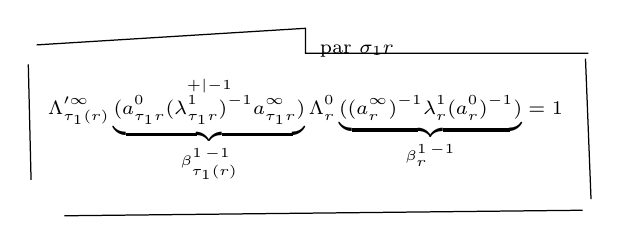
\begin{tikzpicture}[baseline=(live.base)]
\node[inner xsep=5pt,inner ysep=8pt,font=\scriptsize] (live)
 {$\displaystyle \Lambda_{\tau_1(r)}^{\prime\infty}\underbrace{(a_{\tau_1r}^{0}(\lambda_{\tau_1r}^1)^{-1}a_{\tau_1r}^{\infty})}_{\beta_{\tau_1(r)}^{1\,\deleted{\unsure{-1}}}}^{\unsure{+|-1}}\Lambda_r^0\underbrace{((a_r^\infty)^{-1}\lambda_r^1(a_r^0)^{-1})}_{\beta_r^{1\,-1}}=1$};
% Last words of the cancelled NB cross the new upper border at its notch.
\node[anchor=base west,inner sep=0pt,font=\scriptsize] at ([xshift=5pt]live.north)
 {par $\sigma_1r$};
\draw[line width=.45pt] ([xshift=1pt,yshift=3pt]live.north west)
 -- ([yshift=9pt]live.north) -- (live.north)
 -- ([xshift=4pt]live.north east);
\draw[line width=.45pt] ([xshift=3pt,yshift=-2pt]live.north east)
 -- ([xshift=5pt,yshift=2pt]live.south east);
\draw[line width=.45pt] ([xshift=2pt,yshift=-2pt]live.south east)
 -- ([xshift=11pt,yshift=-4pt]live.south west);
\draw[line width=.45pt] ([xshift=-2pt,yshift=-4pt]live.north west)
 -- ([xshift=-1pt,yshift=9pt]live.south west);
\end{tikzpicture}
\]
\margin{relation stable par passage de $r$ à $\tau_1(r)$, donc il suffit de la poser pour $r\in\mathcal{R}^+$ (si $X$ orientable)}
\figure{
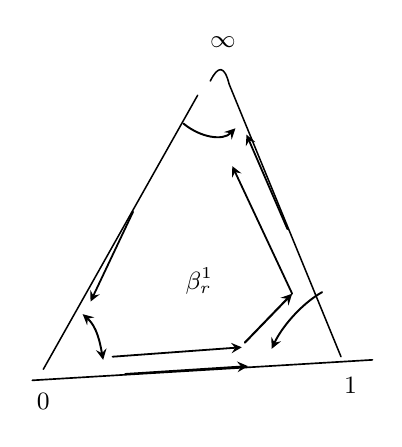
\begin{tikzpicture}[x=.020cm,y=-.020cm,>=stealth,line cap=round,line join=round]
% The side ends remain separate at the 0 and infinity corners.
\draw[line width=.55pt] (129,2127)--(31,2301);
\draw[line width=.55pt] (137,2118)..controls(142,2108)and(146,2108)..(149,2120)
 --(220,2293);
\draw[line width=.6pt] (24,2308)--(240,2295);
% Directions on the three outer sides.
\draw[line width=.65pt,->] (88,2201)--(61,2258);
\draw[line width=.7pt,->] (83,2304)--(161,2299);
\draw[line width=.65pt,->] (186,2212)--(160,2152);
% Interior path: a head at the bend as well as the upper endpoint.
\draw[line width=.65pt,->] (75,2293)--(157,2287);
\draw[line width=.75pt,->] (159,2284)--(189,2253);
\draw[line width=.65pt,->] (189,2253)--(151,2172);
% Three corner arcs, with both heads on the lower-left one.
\draw[line width=.7pt,->] (120,2145)..controls(131,2154)and(145,2156)..(153,2148);
\draw[line width=.7pt,<->] (56,2266)..controls(65,2274)and(67,2284)..(69,2295);
\draw[line width=.7pt,->] (208,2252)..controls(194,2260)and(182,2275)..(176,2288);
\node[font=\small] at (130,2245) {$\beta_r^1$};
\node[font=\small,above] at (145,2103) {$\infty$};
\node[font=\small,below] at (31,2310) {$0$};
\node[font=\small,below] at (226,2300) {$1$};
\end{tikzpicture}
}

\scanpage{120}
\mspage{5}

On a donc trouvé $4=1+3$ présentations du groupoïde fondamental $\Pi_1(\widetilde{X}^{\substack{*\\*}*},S)$, suivant qu'on utilise tous les chemins $(8)$, $(9)$, ou qu'on élimine les chemins $a_r^i$ 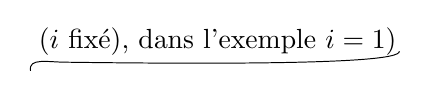
\begin{tikzpicture}[baseline=(base)]
\coordinate (base) at (0,-.22);
\node[anchor=south west,inner sep=0pt] (fixed) at (0,0) {\inserted{($i$ fixé), dans l'exemple $i=1$)}};
\draw[line width=.35pt] ([xshift=-.10cm,yshift=-.19cm]fixed.south west)
 ..controls ([xshift=-.13cm,yshift=-.02cm]fixed.south west) and ([xshift=.12cm,yshift=-.08cm]fixed.south west)..([xshift=.35cm,yshift=-.08cm]fixed.south west)
 ..controls ([xshift=-.40cm,yshift=-.13cm]fixed.south east) and ([xshift=.04cm,yshift=-.02cm]fixed.south east)..([xshift=.03cm,yshift=.06cm]fixed.south east);
\end{tikzpicture} et les sommets qui se trouvent dessus. Je vais maintenant examiner le cas où on élimine $=$ deux côtés du triangle fondamental i.e. où on ne garde les $a_r^i$ que d'un seul type --- disons les $a_r^\infty$ --- ce qui conduit aussi : éliminer tous les sommets proches des $R_\varphi$ 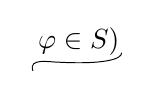
\begin{tikzpicture}[baseline=(base)]
\coordinate (base) at (0,-.20);
\node[anchor=south west,inner sep=0pt] (phi) at (0,0) {\inserted{$\varphi\in S$)}};
\draw[line width=.35pt] ([xshift=-.06cm,yshift=-.19cm]phi.south west)
 ..controls ([xshift=-.12cm,yshift=-.02cm]phi.south west) and ([xshift=.15cm,yshift=-.08cm]phi.south west)..([xshift=.27cm,yshift=-.08cm]phi.south west)
 ..controls ([xshift=-.20cm,yshift=-.11cm]phi.south east) and ([xshift=.03cm,yshift=-.04cm]phi.south east)..([xshift=.02cm,yshift=.04cm]phi.south east);
\end{tikzpicture} de type 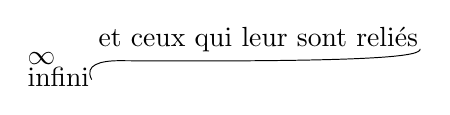
\begin{tikzpicture}[baseline=(infini.base)]
\node[anchor=west,inner sep=0pt] (infini) at (0,0) {\deleted{infini}};
\node[anchor=south west,inner sep=0pt] at (0,.15) {\inserted{$\infty$}};
\node[anchor=south west,inner sep=0pt] (relies) at (.90,.31) {\inserted{et ceux qui leur sont reliés}};
\draw[line width=.35pt] (.82,-.03)
 ..controls (.72,.16) and (.94,.21)..(1.17,.21)
 ..controls ([xshift=-.45cm,yshift=-.12cm]relies.south east) and ([xshift=.03cm,yshift=-.04cm]relies.south east)..([xshift=.02cm,yshift=.05cm]relies.south east);
\end{tikzpicture}, \deleted{\unsure{enfin}, des centres des faces} \inserted{etc.} --- i.e. \deleted{les $R_r^i$} à ne garder que les $R_r^{ij}$ avec \deleted{\unsure{pour}} \inserted{$(i,j)\in\{0,1\}$} \deleted{$\unsure{i,j\ne\infty}$, \unsure{les côtés ne passent pas par $\infty$})} :

\noindent\begin{minipage}[c]{.54\linewidth}
\[
(17)\qquad R_r^{i,j}\quad\left\{\begin{array}{l}
r\in\mathcal{R}\\
\{i,j\}=\{0,1\}
\end{array}\right.
\]
\end{minipage}\hfill
\begin{minipage}[c]{.43\linewidth}
\begin{tikzpicture}[x=1cm,y=1cm]
\node[anchor=west,inner sep=0pt,font=\scriptsize] at (.18,0) {$\left\{\begin{aligned}
R_r^{0,1}&=R_{\tau_\infty r}^{0,1},\\
R_r^{1,0}&=Q_{\tau_\infty(r)}
\end{aligned}\right.$};
\draw[line width=.4pt] (-.05,.65)--(2.5,.8) (-.05,.5)--(-.05,-.65) (.1,-.75)--(4,-.65);
\node[anchor=west,inner sep=0pt,text width=.95cm,font=\scriptsize] at (3.2,.25) {pour mémoire};
\node[anchor=north,inner sep=0pt,text width=2.5cm,align=center,font=\scriptsize] at (2,-.86) {relations de redondance};
\end{tikzpicture}
\end{minipage}

\[
(18)\qquad\left\{\begin{aligned}
a_r^\infty &: \unsure{R_r^{01}|R_r^{0,1}}\underset{\vcenter{\hbox{\begin{tikzpicture}[x=1mm,y=1mm]
\draw[line width=.4pt] (0,0)..controls(2,-.15)and(5,.12)..(7,.12);
\draw[line width=.5pt] (7,-.35)--(7,.62);
\end{tikzpicture}}}}{\deleted{\unsure{\to R}}}R_r^{1,0} \qquad(\forall r\in\mathcal{R})\\
\Lambda_r^0\unsure{,}\deleted{\unsure{\Lambda_r^{\prime1}|\Lambda_r^1}} &:R_r^{01}\longrightarrow\unsure{R_{\tau_1(r)}^{01}|R_{\tau_1r}^{01},}\\
\Lambda_r^{\prime1} &:R_r^{10}\longrightarrow\unsure{R_{\tau_0(r)}^{1,0}|R_{\tau_0r}^{1,0},}
\end{aligned}\right.
\]

\noindent\begin{minipage}[t]{.48\linewidth}
\vspace{0pt}
\figure{
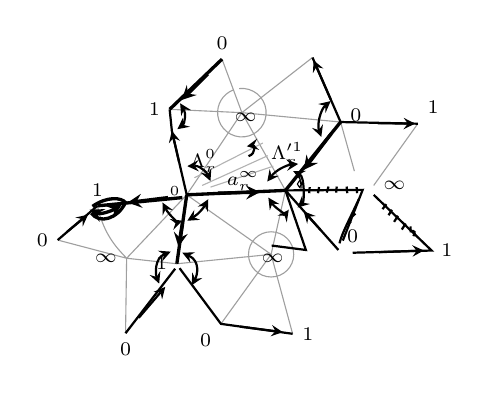
\begin{tikzpicture}[x=.007cm,y=-.007cm,>=stealth,font=\scriptsize]
% Pale triangular construction routes and the two drawn circular contours.
\draw[gray!75] (247,1588)--(378,1594)--(557,1611)
  (342,1497)--(378,1594)--(457,1735)--(278,1743)--(378,1594)--(506,1494);
\draw[gray!75] (116,1763)..controls(128,1817)and(153,1841)..(169,1858)
  (44,1825)--(169,1858)--(167,1994) (169,1858)--(260,1868)
  (169,1858)--(278,1743)--(431,1851)--(260,1868);
\draw[gray!75] (457,1735)--(431,1851)--(340,1977)
  (431,1851)--(470,1995) (557,1611)--(582,1700) (617,1726)--(697,1614);
% The upper pale ring stops on both sides of the spoke; its gap is not closed.
\draw[gray!75] (373.0,1550.3) arc[start angle=-96.5,end angle=248.5,radius=44];
\draw[gray!75] (431,1851) circle (41);
\draw[gray!60] (292,1712)--(416,1649) (306,1726)--(425,1672) (321,1729)--(435,1691);
% Upper left and upper right boundaries; heads lie along the full contours.
\draw[very thick] (342,1497)--(247,1588);
\draw[very thick,->] (316,1524)--(269,1571);
\draw[thick] (278,1743)--(251,1627)--(247,1588);
\draw[thick,->] (264,1683)--(251,1627);
\draw[thick,<->] (266,1577)..controls(277,1595)and(274,1614)..(261,1624);
\draw[thick] (557,1611)--(506,1494);
\draw[thick,->] (539,1570)--(508,1499);
\draw[thick,<->] (539,1573)..controls(521,1588)and(514,1615)..(522,1638);
\draw[thick] (557,1611)--(697,1614);
\draw[thick,->] (624,1613)--(692,1614);
\draw[very thick] (557,1611)--(457,1735);
\draw[very thick,->] (540,1632)--(490,1698);
% The three full dark routes from the central-left junction.
\draw[very thick] (278,1743)--(457,1735);
\draw[very thick,->] (334,1740)--(411,1738);
\draw[very thick] (278,1743)--(260,1868);
\draw[very thick,->] (270,1795)--(263,1837);
\draw[very thick] (270,1748)--(116,1763);
\draw[very thick,->] (244,1748)--(171,1757);
\draw[thick,<->] (279,1691)..controls(305,1690)and(316,1706)..(321,1718);
\draw[thick,<->] (424,1719)..controls(440,1698)and(459,1689)..(480,1687);
\draw[thick,<->] (234,1757)..controls(247,1782)and(264,1792)..(270,1790);
\draw[thick,<->] (279,1790)..controls(301,1777)and(310,1764)..(317,1751);
% Southeast contours: the outer ray points back toward the central junction.
\draw[thick] (457,1735)--(494,1843)--(432,1835);
\draw[thick] (457,1735)--(553,1843);
\draw[thick,->] (521,1807)--(490,1773);
\draw[thick,<->] (471,1700)..controls(492,1710)and(491,1755)..(479,1766);
\draw[thick,<->] (426,1748)..controls(439,1768)and(458,1777)..(463,1770);
% Hatched right-hand routes, preserving the doubled oblique trace.
\draw[thick] (457,1735)--(597,1734)--(561,1826);
\draw[thick] (590,1751)..controls(575,1784)and(559,1813)..(555,1831);
\draw[thick] (501,1729)--(500,1740) (518,1729)--(516,1740)
  (535,1728)--(532,1739) (550,1728)--(549,1739)
  (568,1728)--(569,1740) (586,1729)--(587,1740);
\draw[thick] (584,1777)--(577,1783) (576,1791)--(569,1797);
\draw[thick] (617,1743)--(722,1844)--(579,1848);
\draw[thick,->] (627,1847)--(708,1844);
\draw[thick] (640,1760)--(633,1769) (650,1770)--(644,1780)
  (661,1781)--(654,1792) (675,1795)--(668,1806);
\draw[thick] (684,1800)--(684,1809)..controls(691,1807)and(694,1811)..(689,1818);
% Lower fan and its two opposed corner arcs.
% The upright ends separately above the two lower oblique tips beside 1.
\draw[thick] (167,1994)--(257,1877) (265,1876)--(340,1977)--(470,1995);
\draw[thick,->] (191,1966)--(239,1910);
\draw[thick,->] (375,1982)--(452,1992);
\draw[thick,<->] (249,1846)..controls(220,1858)and(221,1886)..(228,1904);
\draw[thick,<->] (270,1848)..controls(303,1863)and(297,1889)..(287,1907);
% Doubled, heavily traced small loop at the far left.
\draw[thick] (44,1825)--(116,1763);
\draw[thick,->] (61,1810)--(99,1779);
\draw[very thick,<->] (102,1770)..controls(122,1779)and(142,1772)..(160,1761);
\draw[very thick] (107,1764)..controls(134,1745)and(160,1748)..(167,1757)
  ..controls(153,1786)and(120,1797)..(105,1776);
\draw[thick,->] (390,1673)..controls(406,1667)and(398,1653)..(387,1655);
% Written labels, including the tiny central-left oval.
\node[above] at (342,1497) {$0$};\node[left] at (247,1588) {$1$};
\node at (385,1602) {$\infty$};\node[right] at (557,1599) {$0$};
\node[above right] at (697,1614) {$\unsure{1}$};
\node[right] at (617,1726) {$\infty$};
\node[above] at (579,1848) {$0$};\node[right] at (722,1844) {$1$};
\node[right] at (470,1995) {$1$};\node[below left] at (340,1977) {$0$};
\node[below] at (167,1994) {$0$};\node[left] at (260,1868) {$1$};
\node[left] at (169,1858) {$\infty$};\node[left] at (44,1825) {$0$};
\node[above] at (116,1763) {$1$};\node at (434,1858) {$\infty$};
\node[above,inner sep=.1pt] at (256,1745) {$\scriptstyle0$};
\node at (308,1682) {$\Lambda_r^0$};\node at (460,1669) {$\Lambda_r^{\prime1}$};
\node at (380,1718) {$a_r^\infty$};
\node[inner sep=0pt] at (483,1724) {$\unsure{\vcenter{\hbox{\tikz[x=1mm,y=1mm,line width=.4pt]{
  \draw (.1,.45)--(.42,.95)--(.68,.48)--(.37,.03)--(.1,.45);
  \draw (.43,.88)..controls(.72,.58)and(.44,.24)..(.56,-.12);
}}}}$};
\end{tikzpicture}
}
pavage par des \begin{tikzpicture}[baseline=(base)]
\coordinate (base) at (0,-.20);
\node[anchor=south west,inner sep=0pt] (faces) at (0,0) {\inserted{faces}};
\draw[line width=.35pt] ([xshift=-.08cm,yshift=-.19cm]faces.south west)
 ..controls ([xshift=-.10cm,yshift=-.02cm]faces.south west) and ([xshift=.12cm,yshift=-.08cm]faces.south west)..([xshift=.26cm,yshift=-.08cm]faces.south west)
 ..controls ([xshift=-.20cm,yshift=-.10cm]faces.south east) and ([xshift=.05cm,yshift=-.03cm]faces.south east)..([xshift=.03cm,yshift=.06cm]faces.south east);
\end{tikzpicture} polygonales de centre des sommets de type $\infty$ --- \raisebox{-.45ex}{$\unsure{\vcenter{\hbox{\tikz[x=1mm,y=1mm]{\draw[line width=.35pt] (0,0)--(.65,.4);}}}}$} les coins de ces polygones étant arrondis pour éviter les trous
\end{minipage}\hfill
\begin{minipage}[t]{.49\linewidth}
\vspace{0pt}
\begin{tikzpicture}[baseline=(base)]
\coordinate (base) at (0,-.20);
\node[anchor=south west,inner sep=0pt] (avec) at (0,0) {\inserted{avec}};
\draw[line width=.35pt] ([xshift=-.05cm,yshift=-.19cm]avec.south west)
 ..controls ([xshift=-.12cm,yshift=-.04cm]avec.south west) and ([xshift=.12cm,yshift=-.07cm]avec.south west)..([xshift=.23cm,yshift=-.07cm]avec.south west)
 ..controls ([xshift=-.17cm,yshift=-.08cm]avec.south east) and ([xshift=.02cm,yshift=-.04cm]avec.south east)..([xshift=.04cm,yshift=.02cm]avec.south east);
\end{tikzpicture} relations de redondance seulement
\[
(19)\quad\begin{tikzpicture}[baseline=(relation.base)]
\node[inner sep=4pt] (relation) {$\begin{aligned}
\Lambda_r^0\Lambda_{\tau_1(r)}^0&=1\\
\Lambda_r^{\prime1}\Lambda_{\tau_0(r)}^{\prime1}&=1
\end{aligned}$};
\draw[line width=.4pt] ([xshift=-.02cm,yshift=.08cm]relation.north west)
 --([xshift=.10cm,yshift=.17cm]relation.north east)
 --([xshift=.11cm,yshift=-.02cm]relation.south east)
 --([xshift=.02cm,yshift=-.11cm]relation.south west);
\draw[line width=.4pt] ([xshift=-.13cm,yshift=-.04cm]relation.north west)
 --([xshift=-.12cm,yshift=.05cm]relation.south west);
\end{tikzpicture}
\]
c'est donc directement exprimé comme un groupoïde libre. Cela fait trois autres présentations de $\Pi_1(X)$, mais sur des ens. de sommets différents, savoir $\Pi_1(\widetilde{X}^{\vcenter{\hbox{\begin{tikzpicture}[x=1mm,y=1mm]
\node[inner sep=0pt] at (0,1.5) {$\scriptstyle *$};
\node[inner sep=0pt] at (1.5,1.5) {$\scriptstyle *$};
\node[inner sep=0pt] at (1.05,.2) {$\scriptstyle *$};
\node[inner sep=0pt] at (.95,-.8) {$\unsure{\vcenter{\hbox{\tikz[x=1mm,y=1mm]{\draw[line width=.35pt] (0,0)--(.35,0);}}}}$};
\end{tikzpicture}}}},S-S_i)$, pour $i=\infty$ (cas explicité] ou $0$ ou $1$.
\end{minipage}

\mspage{119}

\scanpage{121}
\mspage{6}

Je vais donner \begin{tikzpicture}[baseline=(oldcount.base),line cap=round,line join=round]
  \node[anchor=base west,inner sep=0pt] (oldcount) at (0,0) {\deleted{6}};
  \node[anchor=base west,inner sep=0pt] at (-.12,.54) {\inserted{trois}};
  \draw[line width=.4pt] (-.14,-.03)
    .. controls (-.11,.20) and (.14,.29) .. (.46,.38)
    .. controls (.68,.44) and (.92,.56) .. (.98,.61)
    .. controls (1.01,.65) and (.98,.67) .. (.95,.63);
\end{tikzpicture} autres présentations, où on élimine non seulement les pts proches (disons) des \deleted{$\unsure{R_\varphi|R_q}$} sommets de type \begin{tikzpicture}[baseline=(continuation.base),line cap=round,line join=round]
  \node[anchor=base west,inner sep=0pt] at (-.55,0) {$\infty$};
  \node[anchor=base west,inner sep=0pt] at (-.06,-.01) {,};
  \node[anchor=base west,inner sep=0pt] (continuation) at (.28,0)
    {mais aussi ceux proches des sommets};
  \node[anchor=base west,inner sep=0pt,font=\footnotesize] (linkedinsert) at (-.22,.55)
    {\inserted{et les sommets qui leur sont liés \unsure{d'indice|d'arc} $\infty$}};
  \draw[line width=.4pt] (-.26,-.18)
    .. controls (-.18,-.23) and (-.17,.07) .. (-.12,.19)
    .. controls (-.07,.30) and (.02,.31) .. (.15,.31)
    -- ([xshift=-.08cm,yshift=-.12cm]linkedinsert.south east)
    .. controls ([xshift=.08cm,yshift=-.12cm]linkedinsert.south east)
       and ([xshift=.12cm,yshift=-.03cm]linkedinsert.south east)
       .. ([xshift=.03cm,yshift=-.03cm]linkedinsert.south east);
\end{tikzpicture} (disons) de type $1$, en gardant donc que les sommets \begin{tikzpicture}[baseline=(typezero.base),line cap=round,line join=round]
  \node[anchor=base west,inner sep=0pt] (typezero) at (0,0) {de};
  \node[anchor=base west,inner sep=0pt] at (-.35,.55) {\inserted{$R_r^{i.j}$}};
  \draw[line width=.4pt] (-.15,-.04)
    .. controls (-.15,.19) and (-.08,.29) .. (.10,.30)
    .. controls (.25,.31) and (.41,.39) .. (.47,.46)
    .. controls (.49,.49) and (.47,.51) .. (.44,.48);
\end{tikzpicture} type $0$, i.e.
\[
(20)\qquad R_r^{0,1}\ \mathrel{\tikz[baseline=-.6ex,x=1em,y=1em,>=stealth]{\draw (.70,.70)--(.42,.42);\draw[->] (.29,.29)--(0,0);}}\qquad r\in\mathcal{R}
\]
\margin{$\boxed{R_r^{0,1}=R_{\sigma_\infty r}^{01}}$

relations de redondance pour mémoire}
et on introduit les chemins
\[
(21)\qquad\left\{\begin{aligned}
A_r^{0,1}&\overset{\text{def}}{=}(a_{\tau_0r}^\infty)^{-1}(\Lambda_r^{\prime1})^{-1}a_r^\infty:R_r^{0,1}\longrightarrow R_{\sigma_0(r)}^{0,1}\qquad(r\in\mathcal{R})\\
\Lambda_r^0&:R_r^{0,1}\longrightarrow R_{\sigma_1r}^{01}\qquad(r\in\mathcal{R})
\end{aligned}\right.
\]
\margin{plus les chemins déjà connus}
on a les relations de redondance
\[
(22)\qquad\boxed{\left\{\begin{aligned}
\Lambda_{\unsure{\sigma|r}}^0\Lambda_{\sigma_1(r)}^0&=1&&r\in\mathcal{R}\\
A_r^{0,1}A_{\sigma_0(r)}^{0,1}&=1&&r\in\mathcal{R}
\end{aligned}\right.}
\]
\figure{
\begin{tikzpicture}[scale=1.15,>=stealth]
\coordinate (A) at (0,0);\coordinate (B) at (1.75,-0.10);\coordinate (C) at (1.08,1.65);\coordinate (D) at (2.90,1.10);
\draw (A)--(C)--(D)--(B);
% The lower outline stops just short of the vertex labelled 1 in the ink.
\draw (A)--(1.60,-0.09);
\draw (C)..controls(1.55,0.83)and(1.52,0.40)..(B);
\draw[->] (0.81,1.21)--(1.21,1.20);
\draw[->] (1.61,1.43) to[bend left=12] (1.32,1.09);
\draw[->] (0.52,0.05) to[bend right=20] (0.28,0.38);
\draw[->] (0.62,0.05)--(1.16,0.02);
\draw[very thick,<->] (1.19,-.068) to[bend left=22] (1.52,.31);
\draw[->] (1.16,0.02)..controls(1.30,0.67)and(1.78,0.48)..(1.97,0.32);
\draw[->] (2.03,0.38)--(2.46,0.76);
\draw[<->] (2.49,0.79) to[bend left=14] (2.44,1.17);
\fill (1.72,0.42) circle (0.023);
\node[below left] at (A) {$0$};\node[below] at (B) {$1$};\node[above] at (C) {$\infty$};
\node at (0.88,0.73) {$r$};\node at (1.92,1.00) {$\tau_0r$};\node at (1.99,0.58) {$A_r^{0,1}$};
\node[below] at (0.83,-0.10) {$R_r^{01}$};\node[right] at (2.50,0.53) {$R_{\tau_0r}^{01}$};
\end{tikzpicture}
}
et c'est tout : $\Pi_1(\widetilde{X}^{\substack{*\\*}*},\{R_r^{01}\}_{r\in\mathcal{R}})$ est \deleted{engendré} \inserted{présenté} par les sommets et flèches $(20)$ $(21)$, avec les seules relations de redondance $(20)$ $(22)$.

\uline{Bouchage de trous} Dans chacun des quatre cas envisagés, (en fait $10=1+3+3+3$ cas), le ``bouchage'' d'un trou $R_{\unsure{\varphi s|s}}$ $(s\in S=S_0\amalg S_1\amalg S_\infty)$ se fait de façon essentiellement triviale. Dans chacun des quatre cas, il faut, en termes des flèches génératrices choisies, définir \uline{les}

\mspage{120}

\cotefile{143}

\scanpage{2}
\mspage{1}
\textcircled{1} Soit $\overline{\mathbf Q}$ la clôture algébrique de $\mathbf Q$ dans $\mathbf C$.
Si $X=\overline X$ est un schéma sur $\overline{\mathbf Q}$, on considère le
groupe $\mathcal G_{\overline X}$ des automorphismes de $\overline X$ en tant
que schéma absolu. On a une suite
\[
(1)\qquad 1\longrightarrow G_{\overline X}\longrightarrow\mathcal G_{\overline X}\longrightarrow\Gamma
\]
% The upper unresolved cluster and the lower unreadable span are distinct.
\margin{\begin{tabular}{@{}l@{}}
Question : \unsure{\tikz[baseline=-.4ex,x=.6em,y=.6em]{
  \draw (.10,1.20) .. controls (.45,1.75) and (.85,1.70) .. (.70,1.20)
    .. controls (.45,.70) and (.20,.15) .. (-.05,-1.10);
  \draw (.65,1.25) .. controls (1.10,1.65) and (1.20,1.25) .. (.80,.98)
    --(.55,-.45) .. controls (.60,-.10) and (1.12,-.15) .. (1.15,-.50);
  \draw (-.10,.85)--(.80,1.08);
  \draw (-.15,.60) .. controls (.45,.70) and (.65,.55) .. (1.00,.80);
}}\\
\unsure{comment|comme} \illegible{1} ?
\end{tabular}}
où
\[
(2)\qquad\left\{\begin{aligned}
\Gamma&=\operatorname{Gal}(\overline{\mathbf Q}/\mathbf Q)\\
G_{\overline X}&:\operatorname{Aut}(\overline X/\overline{\mathbf Q})
\end{aligned}\right.
\]
% The small subset-shaped curve is detached below the arrow shaft.
\margin{\diagram{\begin{tikzcd}[ampersand replacement=\&,column sep=small]
\overline{\mathbf Q}\arrow[d,phantom,"\cup" description]
\&\mathrel{\tikz[baseline=-.45ex,x=1em,y=1em]{
  \draw[->] (0,0)--(1.8,0);
  \draw (.30,-.12) .. controls (.02,-.12) and (.02,-.35) .. (.30,-.35);
}}
\&\Gamma(X_{\mathrm{red}},\underline{\mathcal O}_X)\\
\mathbf Q\&\&
\end{tikzcd}}
Il faut supposer p.ex. que $\overline{\mathbf Q}$ est la
clôt. int. de $\mathbf Q$ ds $\Gamma_X$}
(3) Les sous-extensions $K$ de $\overline{\mathbf Q}/\mathbf Q$ correspondent
aux sous-groupes fermés $\Gamma_K$ de $\Gamma$ (d'indice
fini ssi $K$ fini sur $\mathbf Q$). À une restriction
du groupe de base $\overline{\mathbf Q}$ de $\overline X$ \unsure{:|à} $K$ correspond
un relèvement
% The upper connector has a shaft and an upper terminal cap, not a complete two-wing head.
\diagram{\begin{tikzcd}[ampersand replacement=\&,column sep=small]
(4)\quad\mathcal G_{\overline X}
\&\mathrel{\tikz[baseline=-.45ex,x=1em,y=1em]{
  \draw (0,0)--(1.8,0);
  \fill (1.8,0)--(1.60,.12)--(1.60,0)--cycle;
}}
\&\Gamma\arrow[d,phantom,"\cup" description]\\
\&\&\Gamma_K\arrow[ull]
\end{tikzcd}\,,}
\margin{grain de sel d'effectivité de descente
\unsure{et l'hypothèse}
\unsure{qu. proj.|gr. proj.}}
qui le définit si $\overline X$ est
\tikz[baseline=(w.base)]{
  \node[inner sep=0pt] (w) at (0,0) {réduit};
  \node[inner sep=0pt] at (.48,.20) {?};
  \draw (.08,.06) ellipse (.73cm and .32cm);
}
et \uline{loc de t f.}
sur $\overline{\mathbf Q}$. Cela montre que si $\overline X$ est de t.f.
\deleted{quasi-proj}
sur $\overline{\mathbf Q}$, l'hom $\mathcal G_{\overline X}
\mathrel{\tikz[baseline=-.45ex,x=1em,y=1em]{
  \draw (0,0)--(1.5,0);
  \fill (1.5,0)--(1.36,.08)--(1.36,0)--cycle;
}}\Gamma$ a une image
d'indice fini (puisqu'on peut
\tikz[baseline=0pt]{
  \node[inner sep=0pt] at (.12,.60) {\inserted{alors}};
  \draw (-.35,-.13) .. controls (-.30,.25) and (.28,.31) .. (.48,.39);
}
réduire le
corps de base à une ext. finie $K$ de $\mathbf Q$).

\textcircled{2} \uline{Supposons $X$ connexe
\tikz[baseline=0pt]{
  \node[inner sep=0pt] at (.18,.53) {\inserted{$\ne\varnothing$}};
  \draw (-.23,-.18) .. controls (-.35,.06) and (.55,.27) .. (.78,.80);
}, et}
Considérons un revêtement universel $\widetilde X\xrightarrow{\unsure{h|b}}X$
$X$, et \deleted{considérons} posons
\[
(5)\qquad \mathcal E(X,\widetilde X)\ \text{ou}\ \mathcal E_X=
\operatorname{Aut}\left(\widetilde X
% Literal overloaded separator; deletion state and interpretation remain doubtful.
\unsure{\mathbin{\tikz[baseline=-.45ex,x=1em,y=1em]{
  \draw[line width=.65pt] (.06,-.32)--(.26,.34);
  \draw[line width=.85pt] (-.03,0)--(.42,0);
  \fill (.42,0)--(.31,.065)--(.31,-.065)--cycle;
}}}X\right)
\]
\mspage{1}

\scanpage{3}
On a donc une suite exacte
\diagram{\begin{tikzcd}[ampersand replacement=\&,column sep=large]
{(6)}\&1\arrow[r]\&\pi_1(X)\arrow[r]\arrow[d,equal]\&\mathcal E_X\arrow[r]\&\mathcal G_X\arrow[r]\arrow[d]\&1\\
\&\&\operatorname{Aut}(\widetilde X/X)\&\&\Gamma\&
\end{tikzcd}}
\deleted{La donnée d'un point}

Considérons un point \unsure{\begin{tikzpicture}[x=.008cm,y=-.008cm,baseline=(xibase.base),line cap=round,line join=round]
\node[inner sep=0pt] (xibase) at (1038,561) {\phantom{$x$}};
% The xi and adjacent X-like overwork are kept at their visible relative positions.
\draw[line width=.55pt] (1022,521)..controls(1037,519)and(1048,516)..(1058,514)
 ..controls(1064,514)and(1054,522)..(1038,526)--(1023,536)
 ..controls(1024,541)and(1048,539)..(1075,534);
\draw[line width=.55pt] (1024,537)..controls(1020,543)and(1030,547)..(1027,555)
 ..controls(1024,566)and(1022,573)..(1025,584)
 ..controls(1038,584)and(1047,587)..(1049,591);
\draw[line width=.65pt] (1025,584)..controls(1028,597)and(1024,603)..(1024,610);
\draw[line width=.5pt] (1073,535)..controls(1069,541)and(1056,544)..(1055,548)
 ..controls(1057,552)and(1063,550)..(1065,551);
\draw[line width=.55pt] (1079,535)..controls(1073,539)and(1070,549)..(1069,555)
 ..controls(1068,562)and(1075,565)..(1081,565);
\draw[line width=.4pt] (1026,579)--(1076,538);
\draw[line width=.55pt] (1079,549)..controls(1083,547)and(1085,548)..(1086,549);
\end{tikzpicture}}
\[
(7)\qquad\xi\in X(\overline{\mathbf Q})
\]
et soit $\mathcal G_X(\xi)\subset\mathcal G_X$ le sous-groupe
de $\mathcal G_X$ qui fixe $\xi$. (NB. Si \begin{tikzpicture}[baseline=(gx.base)]
\node[anchor=base west,inner sep=0pt] (gx) at (1.55,0) {$G_X$};
\node[anchor=base west,inner sep=0pt] (nbinsert) at (0,.62)
 {\inserted{$X$ est de t.f. $/\overline{\mathbf Q}$ et \unsure{sep}}};
% The under-running line bends down on the left to attach before G_X.
\draw[line width=.35pt] ([xshift=-1pt,yshift=-2pt]nbinsert.south east)
 -- ([xshift=-1pt,yshift=-5pt]nbinsert.south east)
 ..controls(3.30,.33)and(2.03,.43)..(1.48,.36)
 ..controls(1.20,.31)and(1.21,.04)..(1.42,-.17);
\end{tikzpicture} est
fini, $\mathcal G_X$ est profini et $\mathcal G_X(\xi)$ est un
s-groupe ouvert\ldots). On trouve alors,
si on choisit pour $\widetilde X$ le rev. universel
\begin{tikzpicture}[baseline=(pointed.base)]
\node[anchor=base west,inner sep=0pt] (pointed) at (.75,0) {pointé};
\node[anchor=base west,inner sep=0pt] at (.02,.50) {\inserted{$\widetilde X(\xi)$}};
\draw[line width=.35pt] (.92,.34)..controls(.66,.12)and(.23,.23)..(.10,-.18);
\end{tikzpicture} au dessus de $\xi$, un
splitting partiel de (6)
\diagram{
\begin{tikzpicture}[>=stealth,line cap=round,line join=round]
\node at (-2.15,-.28) {$(8)$};
\node[inner sep=0pt] (ex) at (0,0) {$\mathcal E_X$};
\node[inner sep=0pt] (gg) at (2.45,0) {$\mathcal G_X$};
\node[inner sep=0pt] at (4.20,0) {$1$};
\node[inner sep=0pt] (stab) at (2.52,-1.52) {$\mathcal G_X(\xi)$};
\draw[line width=.65pt,->] (.46,0)--(1.88,0);
% The right horizontal stroke ends in a short downward tick, not a two-wing head.
\draw[line width=.55pt] (3.03,0)--(3.69,0)--(3.69,-.055);
% Tall open U with the left arm longer than the right; no arrowhead is supplied.
\draw[line width=.6pt] (2.48,-.41)..controls(2.46,-.74)and(2.46,-1.05)..(2.54,-1.08)
 ..controls(2.59,-1.06)and(2.65,-.91)..(2.68,-.80);
\draw[line width=.65pt,->] (1.93,-1.23)--(.26,-.48);
\end{tikzpicture}
}
Dans le cas où $\widetilde X$ est quelconque, on
ne trouve qu'un hom. mod composition
avec autom intérieurs provenant de
$\pi_1(X)$. \deleted{Si $X$ est de t.f. et}
\mspage{2}

\scanpage{4}
\mspage{2}
\figure{
\begin{tikzpicture}[x=.009cm,y=-.009cm,font=\small]
% The cancelled passage has three separate enclosing strokes, not a closed box.
\node[anchor=west,inner sep=0pt] at (240,125) {\deleted{s'envoie injectivement dans un groupe algébrique}};
\node[anchor=west,inner sep=0pt] at (240,215) {\deleted{commutatif de rang unipotent nul}};
\node[anchor=west,inner sep=0pt] at (250,305) {\deleted{(i.e. ext. d'une VA par un tore) alors}};
\node[anchor=west,inner sep=0pt] at (260,412) {\deleted{\uline{l'application}}};
\node[anchor=west,inner sep=0pt] at (570,480) {\begin{tikzcd}[ampersand replacement=\&,column sep=18mm]
{\deleted{X(\overline{\mathbf Q})}}\arrow[r]\&{\deleted{J}}
\end{tikzcd}};
\draw[line width=.4pt] (230,130)..controls(650,100)and(1190,99)..(1580,125);
\draw[line width=.4pt] (245,155)..controls(235,230)and(223,350)..(224,392)
 ..controls(224,406)and(228,412)..(233,402);
\draw[line width=.4pt] (526,440)..controls(520,466)and(516,501)..(531,516)
 ..controls(590,536)and(730,507)..(945,513)
 ..controls(929,475)and(922,387)..(922,348)
 ..controls(1010,330)and(1365,347)..(1552,329);
% Oblique cancellation is retained as physical ink, not counted as another error.
\draw[line width=.35pt] (484,140)--(367,371) (837,126)--(572,488)
 (1094,142)--(814,468) (1436,148)--(1258,296) (1577,153)--(1514,284);
\end{tikzpicture}
}

\textcircled{3} Supposons $X$ de t.f. sur $\overline{\mathbf Q}$. Alors on a
un ``germe de relèvement'' de $\Gamma$
\diagram{$(9)\qquad$
\begin{tikzcd}[ampersand replacement=\&]
\mathcal G_{\overline X}\arrow[r]\&\Gamma\arrow[d,phantom,"\cup" description]\\
\&\Gamma'\arrow[ul]
\end{tikzcd}}

sur ss-groupe ouvert (modulo la relation
de coïncidence sur un ss groupe
ouvert plus petit). Pour \begin{tikzpicture}[baseline=(base)]
\coordinate (base) at (0,-.23);
\node[anchor=south west,inner sep=0pt] (xinote) at (0,0) {\inserted{$\xi\in X(\overline{\mathbf Q})$ donné, et pour}};
\draw[line width=.35pt] ([xshift=-.05cm,yshift=-.22cm]xinote.south west)
 ..controls ([xshift=-.13cm,yshift=-.08cm]xinote.south west) and ([xshift=-.04cm,yshift=-.02cm]xinote.south west)..([xshift=.12cm,yshift=-.03cm]xinote.south west)
 ..controls ([xshift=-.50cm,yshift=.01cm]xinote.south east) and ([xshift=-.20cm,yshift=-.08cm]xinote.south east)..([xshift=.01cm,yshift=-.08cm]xinote.south east);
% Only the definite sweep is copied; its far-right extent merges with crease/edge.
\end{tikzpicture}
$\Gamma'$ assez petit,
\inserted{de $\xi$} $\Gamma'
\mathrel{\vcenter{\hbox{\begin{tikzpicture}[x=1mm,y=1mm]
\draw[line width=.45pt] (0,0)--(6,0)--(6,-.4);
\end{tikzpicture}}}}
\mathcal G_{\overline X}$ se factorise par $\mathcal G_{\overline X}(\xi)$, de
\margin{$X=\overline X$}
sorte qu'on a un \begin{tikzpicture}[baseline=(base)]
\coordinate (base) at (0,-.22);
\node[anchor=south west,inner sep=0pt] (germe) at (0,0) {\inserted{germe d'}};
\draw[line width=.35pt] ([xshift=-.06cm,yshift=-.20cm]germe.south west)
 ..controls ([xshift=-.17cm,yshift=-.08cm]germe.south west) and ([xshift=-.02cm,yshift=-.02cm]germe.south west)..([xshift=.18cm,yshift=-.03cm]germe.south west)
 ..controls ([xshift=-.40cm,yshift=-.10cm]germe.south east) and ([xshift=-.15cm,yshift=.01cm]germe.south east)..([xshift=.02cm,yshift=.05cm]germe.south east);
\end{tikzpicture} hom composé
\[
\begin{gathered}
\hspace{1.6cm}\inserted{\Gamma'\mathrel{\vcenter{\hbox{\begin{tikzpicture}[x=1mm,y=1mm]
\draw[line width=.45pt,line cap=round] (0,0)..controls(2,.12)and(5,.48)..(6.6,.32);
\draw[line width=.45pt,line cap=round] (7,.8)--(7.3,.2)--(6.95,-.1);
\end{tikzpicture}}}}\mathcal E_X}\\[-.2em]
\deleted{\Gamma'\longrightarrow\mathcal E_X}\hspace{1.6cm}
\end{gathered}
\]
rendant commutatif
\diagram{$(10)\qquad$
\begin{tikzcd}[ampersand replacement=\&]
\mathcal E_X\arrow[r]\&\mathcal G_X\arrow[r]\&\Gamma\\
\&\&\Gamma'\arrow[u,hook]\arrow[ull,"{\varphi_\xi^t}"{below}]
\end{tikzcd}}

-- du moins si $\widetilde X=\widetilde X(\xi)$ -- sinon un
hom defini mod composition par un \unsure{autom}
int. provenant de $\pi_1(X)$. \unsure{Soulignons}
\mspage{3}

\scanpage{5}
encore une fois que c'est le \uline{germe}
seulement des $\varphi_\xi$ qui est défini
(mod restriction à ss groupe d'indice
fini). [Si $X$ s'envoie injectivement
dans une extension d'une VA par un
tore, alors $\xi$ est connu quand on
connait ce germe
\[
(11)\qquad\varphi_\xi\in\underset{\substack{\Gamma'\subset\Gamma\\\text{ouvert}}}{\lim\limits_{\longrightarrow}}
\operatorname{Hom}(\Gamma',\begin{tikzpicture}[baseline=(ext.base)]
\node[inner sep=0pt] (ext) at (0,0) {$\mathcal E$};
\node[anchor=base west,inner sep=0pt,font=\scriptsize] at (.20,-.10)
 {$\deleted{\unsure{\overline X}}$};
\node[inner sep=0pt,font=\scriptsize] at (.03,-.43) {$\inserted{X}$};
\end{tikzpicture})
/\operatorname{Int}(\pi_1(X),\mathcal E_X)
\]
[et $=$ l'image de $\varphi_\xi$ dans un $H^1$ abélien
convenable\ldots] ]

\textcircled{4}
\[
(12)\qquad\text{Soit }\begin{tikzpicture}[baseline=(div.base),line cap=round,line join=round]
\node[inner sep=0pt] (div) at (2.15,0) {$\displaystyle D=\sum_{i\in I}D_i$};
% Open underneath: left outward foot, rounded roof, curled right foot.
\draw[line width=.45pt] (-.10,-.53)--(.50,-.53)
 ..controls(.37,-.20)and(.29,.48)..(.70,.64)
 ..controls(1.80,.89)and(3.20,.86)..(3.88,.79)
 ..controls(3.86,.40)and(3.66,-.30)..(4.00,-.36)
 ..controls(4.10,-.41)and(4.22,-.38)..(4.31,-.38);
\end{tikzpicture}\quad\text{un diviseur }\begin{tikzpicture}[baseline=(sur.base)]
\node[anchor=base west,inner sep=0pt] (sur) at (.48,0) {sur $X$,};
\node[anchor=base west,inner sep=0pt] at (-.34,.60) {\inserted{effectif}};
\draw[line width=.35pt] (-.38,.35)..controls(-.39,.17)and(.34,.32)..(.40,.04)
 ..controls(.45,-.07)and(.43,-.15)..(.39,-.20);
\end{tikzpicture}
\]
($I$ l'ens de ses comp. irréd) sans comp. mult.,
supposons que $X$ soit régulier \begin{tikzpicture}[baseline=(enles.base)]
\node[anchor=base west,inner sep=0pt] (enles) at (.63,0) {en les};
\node[anchor=base west,inner sep=0pt] at (-.10,.61) {\inserted{(i.e. lisse)}};
\draw[line width=.35pt] (1.61,.42)..controls(1.30,.15)and(.57,.40)..(.36,.09)
 ..controls(.25,-.05)and(.26,-.16)..(.27,-.23);
\end{tikzpicture}
pts gén. de chaque $D_i$. Soit \deleted{$X_I$}
\[
(13)\qquad X'=X-\operatorname{supp}D
\]
et considérons le sous-groupe $\mathcal G_{\unsure{X',X|X;X}}$ de
$\mathcal G_X$ qui invarie $D$. On le notera \begin{tikzpicture}[baseline=(par.base)]
\node[anchor=base west,inner sep=0pt] (par) at (.61,0) {(par};
\node[anchor=base west,inner sep=0pt] at (.05,.53) {\inserted{encore}};
\draw[line width=.35pt] (1.07,.40)..controls(.89,.22)and(.35,.26)..(.12,-.06);
\end{tikzpicture}
abus de notation) $\mathcal G_{X'}$, \begin{tikzpicture}[baseline=(alors.base)]
\node[anchor=base west,inner sep=0pt] (alors) at (.47,0) {Alors on a};
\node[anchor=base west,inner sep=0pt] (refinement) at (-.19,.67)
 {\inserted{\unsure{--|ou} plus précisém\unsure{ent|t} $\mathcal G_{X'}(I)$.}};
\draw[line width=.35pt] ([xshift=-1pt,yshift=-2pt]refinement.south east)
 ..controls(3.55,.33)and(1.65,.46)..(.43,.42)
 ..controls(.12,.37)and(.02,-.16)..(.18,-.26);
\end{tikzpicture}
\mspage{4}

\scanpage{6}
\mspage{3}
\[
(14)\qquad
1\mathrel{\vcenter{\hbox{\begin{tikzpicture}[x=1mm,y=1mm]
\draw[line width=.45pt] (0,0)--(3,0);
\draw[line width=.6pt] (3,.1)--(3,-.22);
\end{tikzpicture}}}}\pi_1(X')
\mathrel{\vcenter{\hbox{\begin{tikzpicture}[x=1mm,y=1mm]
\draw[line width=.45pt] (0,0)--(6,0);
\draw[line width=.65pt] (6,.24)--(6,-.24);
\end{tikzpicture}}}}\mathcal E_{X'}
\longrightarrow\mathcal G_{X'}\longrightarrow1.
\]
et on a encore un germe de \deleted{hom} \inserted{relèvement}
\unsure{Circonstanciellement|circonstanciellement} mod comp. par autom int.
provenant de $\pi_1(X')$)
\diagram{$(15)\qquad$
\begin{tikzcd}[ampersand replacement=\&]
\mathcal E_{X'}\arrow[r,phantom,
"{\vcenter{\hbox{\begin{tikzpicture}[x=1mm,y=1mm]
\draw[line width=.45pt] (0,0)--(6,0)--(6,.5);
\end{tikzpicture}}}}" description]
\&\mathcal G_{X'}\arrow[r]\&\Gamma\arrow[d,phantom,"\cup" description]\\
\&\&\Gamma'\arrow[ull,"{\varphi_\xi}"{below}]
\end{tikzcd}}
(si $\xi\in X'(\overline{\mathbf Q})$).

Notons qu'on a ici un hom
\[
(16)\qquad\mathcal G_{X'}\longrightarrow\mathfrak S_I
\]
La théorie de Kummer nous fournit,
pour $\forall\,i$, un hom extérieur
\diagram{%
\begin{tikzpicture}[x=1cm,y=1cm,line width=.45pt]
\node at (-2.45,-.64) {$(17)$};
\node (t17) at (0,0) {$\mathbf T(\overline{\mathbf Q})$};
\node at (4.75,0) {$\pi_1(X')$};
\draw[->] (1.08,0)--(3.83,0);
% The phi_i label's own long stem crosses the horizontal shaft.
\draw (2.45,-.25)--(2.45,.61)
 .. controls (2.29,.73) and (2.43,.97) .. (2.56,.99);
\draw (2.45,.61)
 .. controls (2.56,.55) and (2.72,.65) .. (2.68,.80)
 .. controls (2.63,.94) and (2.46,.86) .. (2.45,.61);
\node[anchor=west] at (2.75,.53) {$\scriptstyle i$};
\draw[->] (-.10,-.34)
 .. controls (-.26,-.58) and (-.18,-.89) .. (.16,-.87);
\node[anchor=base west] at (-.44,-1.22) {$=$};
\node[anchor=base west] at (.02,-1.22)
 {$\displaystyle\varprojlim\mu_n(\overline{\mathbf Q})$};
\end{tikzpicture}}
\margin{$\varphi_i\in\operatorname{Homext}
(\mathbf T(\unsure{\mathbf Q|\overline{\mathbf Q}}),\pi_1(X'))$}
{\reversemarginpar
\margin{\deleted{il faut supposer $\chi=1$
\unsure{si l'on veut}
\unsure{interpréter ça par} \illegible{?}
\unsure{purement arithmétique}
\unsure{un objet} \unsure{\dots}}}
\normalmarginpar}

Notons aussi un hom canonique
\[
(18)\qquad
\left(\mathcal G_{X'}
\mathrel{\vcenter{\hbox{\begin{tikzpicture}[x=1mm,y=1mm]
\draw[line width=.45pt] (0,0)--(5.5,0)--(5.55,.22)--(5.7,0);
\end{tikzpicture}}}}\right)
\Gamma\xrightarrow{\chi}\widehat{\mathbb Z}^{*}
\xrightarrow{\sim}\operatorname{Aut}(\mathbf T(\overline{\mathbf Q}))
\]
faisant opérer $\mathcal G_{X'}$ via $\Gamma$ sur $\mathbf T(\overline{\mathbf Q})$.
Ceci dit, l'\unsure{opération|Opération} extérieure de $\mathcal G_{X'}$
sur $\pi_1(X')$ est compatible avec la famille
\mspage{5}

\scanpage{7}
des $(\varphi_i)$ (``structure Kummérienne'')
compte tenu des opérations
\tikz[baseline=0pt]{
  \node[inner sep=0pt] at (.10,.52) {\inserted{(16) et (18)}};
  \draw (-.62,-.12) .. controls (-.66,.26) and (-.48,.35) .. (-.20,.35)
    .. controls (.36,.35) and (.55,.27) .. (.78,.34);
}
de $\mathcal G_{X'}$
sur $I$ et $\mathbf T(\overline{\mathbf Q})$. On peut donc
écrire
\[
(19)\qquad\mathcal G_{X'}\longrightarrow
\operatorname{Autext}\bigl(\pi_1(X'),\mathbf T(
\unsure{\tikz[baseline=-.4ex,x=1em,y=1em]{
  \draw (-.05,.87)--(.72,.89);
  \draw (.17,.64) .. controls (.03,.39) and (.03,.03) .. (-.10,-.38);
  \draw (.23,.30) .. controls (.46,.72) and (.78,.63) .. (.58,.24)
    .. controls (.42,-.04) and (.18,-.05) .. (.16,.20);
  \draw[line width=.65pt] (.10,.09) .. controls (.25,-.11) and (.43,.02) .. (.54,.18);
  \draw[line width=.65pt] (.23,.12)--(.20,-.16);
  \fill (.72,.34) circle (.035);
  \draw[line width=.65pt] (.62,.17)--(.64,-.16);
}}
),(\varphi_i)\bigr).
\]
\deleted{Supposons $X$}
% This looped trace may be a cancellation return; no additional word is supplied.
\unsure{\tikz[baseline=-.4ex,x=1em,y=1em]{
  \draw (-.30,.40)--(1.35,.40);
  \draw (-.55,.10)--(1.18,.10);
  \draw (.15,.30) .. controls (.87,.35) and (1.10,.29) .. (1.13,.15)
    .. controls (.94,.03) and (.84,.04) .. (.80,.10);
  \draw (.45,-.03) .. controls (.80,.03) and (1.03,-.05) .. (1.37,.02);
}}

Soit $\widehat{\widetilde X'}$ le normalisé de
% Cancelled cluster above the live X; the underlying decoration remains uncertain.
$\overset{\unsure{\tikz[baseline=0pt,x=1em,y=1em]{
  \draw (0,.17) .. controls (.14,.42) and (.25,.07) .. (.43,.22)
    .. controls (.58,.40) and (.70,.11) .. (.82,.20);
  \draw[line width=.7pt] (-.03,.10)--(.34,.39)--(.09,.13)--(.48,.39)
    --(.22,.11)--(.69,.35)--(.45,.08)--(.89,.29);
  \draw[line width=.7pt] (.87,.18)--(.66,-.02)--(.84,-.08)--(.78,-.20);
}}}{X}$ dans ``l'extension''
definie par $\widetilde X'$, donc on a un
morphisme profini
\[
\widehat{\widetilde X'}\longrightarrow X
\]
Soit $\widetilde X'(I)$ l'image inverse de l'ens des
pts \deleted{génériques} \inserted{maximaux} des $D=\sum D_i$. On a
donc
\[
(20)\qquad\widetilde X'(I)
\mathrel{\tikz[baseline=-.45ex,x=1em,y=1em]{
  \draw (0,0)--(1.80,0);
  \draw[line width=.65pt] (1.80,0) .. controls (1.82,.12) and (1.75,.15) .. (1.73,.035);
}}I
\]
et une opération de $\deleted{\unsure{\mathcal G_{X'}|\mathcal G_X}}\mathcal E_{X'}$ sur
$\widetilde X'(I)$ qui transporte \unsure{de|la} structure)
compatible avec les opérations sur $I$
et l'application (20). Pour $i\in I$) soit
\[
(21)\qquad\widetilde X'(i)\subset\widetilde X'(I)
\]
sa fibre dans $\widetilde X'(I)$,
% Physical cluster: on versus a leader end remains unresolved.
\unsure{\tikz[baseline=-.35ex,x=1em,y=1em]{
  \draw (.03,.04) .. controls (-.07,.22) and (.23,.27) .. (.16,.04)
    .. controls (.11,-.06) and (-.02,-.02) .. (.03,.04);
  \draw (-.08,.17)--(.12,.34);
  \draw (.20,.05) .. controls (.28,.23) and (.37,.18) .. (.37,.05)
    --(1.25,.01) .. controls (1.37,.01) and (1.41,-.02) .. (1.45,-.08);
}}
\margin{\begin{tikzpicture}[x=1em,y=1em]
  \node[anchor=west,inner sep=0pt] at (.35,1.75) {C'est un espace hom.};
  \node[anchor=west,inner sep=0pt] at (.85,.85) {sous $\pi_1(X')$. On};
  \node[anchor=west,inner sep=0pt] at (.95,-.05) {trouve.};
  \node[anchor=west,inner sep=0pt] at (5.70,-.05) {alors};
  % Left parenthetical/enclosing curve, locally retraced at its lower turn.
  \draw (-.05,2.18) .. controls (-1.05,1.85) and (-1.00,.85) .. (-.65,.55)
    .. controls (-.15,.10) and (.02,-.18) .. (.14,-.48);
  \draw (-.66,.62) .. controls (-.18,.48) and (.01,-.12) .. (.14,-.48);
  % Continuing enclosure/attachment stroke; this does not delete the lower words.
  \draw (.45,-.43) .. controls (.05,-.08) and (.66,.25) .. (1.10,.25)
    .. controls (4.25,.34) and (7.20,.10) .. (8.65,.53)
    .. controls (8.83,.66) and (8.78,.86) .. (9.05,.94);
\end{tikzpicture}}
\mspage{6}
